%!TEX TS-program = pdflatex
%!TEX encoding   = UTF-8 Unicode
%!BIB TS-program = biber

\documentclass{uosthesis}

\usepackage[utf8]{inputenc}
\usepackage[british]{babel}
\usepackage[sb]{libertinus}
\usepackage[T1]{fontenc}
\usepackage{textcomp,amssymb,mathtools,accents}
\usepackage[varqu,varl,scaled=.95]{inconsolata}
\usepackage[amsthm,subscriptcorrection,frenchmath]{libertinust1math}
\usepackage[scr=boondoxo,bb=boondox]{mathalpha}
\usepackage[hyphenation,parindent,lastparline,rivers]{impnattypo}
\usepackage[mathcal]{euscript}
\usepackage{bm}
\usepackage[style=ext-authoryear-ecomp,hyperref,backref]{biblatex}
\usepackage[style=british]{csquotes}
\usepackage{bookmark,titlesec,enumitem}
\usepackage[font=small,labelfont=bf,labelsep=quad,justification=justified,singlelinecheck=off]{caption}
\usepackage[ruled,vlined,linesnumbered,resetcount,algochapter]{algorithm2e}
\usepackage[all]{nowidow}
\usepackage{emptypage,pgfplots,addlines,environ,nameref,tocbasic,tocloft}
\usepackage[normalem]{ulem}
\usepackage[nomain,acronyms,toc=false,section=section,nonumberlist,style=mcoltree,stylemods={mcols,longbooktabs}]{glossaries-extra}
\usepackage[activate={true,nocompatibility},final,babel=true,tracking=true,kerning=true,spacing=true]{microtype}

\usepackage{silence}
\WarningFilter{microtype}{I cannot find a spacing list}
\WarningFilter{microtype}{Unable}
\WarningFilter{latexfont}{Font shape}
\WarningFilter{latexfont}{Some font}
\WarningFilter{glossaries}{No}

\pgfplotsset{compat=1.18}
\usetikzlibrary{pgfplots.groupplots,patterns,shapes.geometric,arrows.meta,plotmarks,pgfplots.fillbetween}

\pgfplotscreateplotcyclelist{exotic2}{%
    black!5!red, densely dashed, every mark/.append style={solid,fill=red!45},mark=*\\%
    black!5!orange, every mark/.append style={fill=white},mark=square*\\%
    blue!80, every mark/.append style={fill=blue!45},mark=triangle*\\%
}

\pgfplotscreateplotcyclelist{exotic3}{%
    black!5!red,every mark/.append style={solid,fill=red!80!black},mark=diamond*\\%
    blue!45,every mark/.append style={fill=blue!45},mark=otimes*\\%
    blue!90,densely dashed,mark=asterisk,every mark/.append style=solid\\%
}

% https://tex.stackexchange.com/a/308647
\let\isout\sout
\renewcommand{\sout}[1]{\ifmmode\text{\isout{\ensuremath{#1}}}\else\isout{#1}\fi}

\definecolor{mycol1}{HTML}{008000} % green
\definecolor{mycol2}{HTML}{FF8000} % orange

\graphicspath{{./images/}}

\numberwithin{figure}{chapter}
\numberwithin{equation}{chapter}
\numberwithin{table}{chapter}

\renewcommand{\headrulewidth}{0pt}

\fancypagestyle{plain}{
		\fancyhead{}
		\fancyfoot{}
		\fancyfoot[C]{\thepage}
}

\fancypagestyle{references}{
    \fancyhead[LO,RE]{References}
    \fancyhead[RO,LE]{\thepage}
		\fancyfoot{}
}

\titleformat{\chapter}[display]%
{\normalfont\huge\bfseries\raggedright}{\normalfont\LARGE\chaptertitlename\ \thechapter}{20pt}{\Huge}

\setcounter{tocdepth}{2} % set 2 to show subsections
\setcounter{secnumdepth}{3}
%\counterwithout*{footnote}{chapter}

\defglsentryfmt[acronym]{\textit{\glsentrylong{\glslabel}} (\glsentrytext{\glslabel})}
\newglossary{symbols}{sym}{sbl}{Symbols}
\makenoidxglossaries
\loadglsentries{sections/glossary.tex}
\glsaddall
\glssetcategoryattribute{acronym}{nohyper}{true}
\renewcommand*{\glsnamefont}[1]{\textbf{#1}}
\renewcommand{\glossarypreamble}{\small}

\DeclareNameAlias{default}{family-given}
\addbibresource{references.bib}
\renewcommand*{\bibfont}{\small}
\DeclareOuterCiteDelims{cite}{\bibopenbracket}{\bibclosebracket}

\SetKwComment{Comment}{\hspace{.3em}// }{} % [l,r] options append \; by default
\SetKw{Break}{break}
%\SetAlgoCaptionSeparator{$\;\;$}

\newcommand{\alloc}[2]{\tau^{#1 \rightarrow v}_{#2}}
\newcommand{\tmax}{t_{max}}
\newcommand{\mxc}{x_{v,\, t,\, C}}
\newcommand{\mxa}{x_{v,\, t,\, a}}
\newcommand{\mx}{x_{v,\, l,\, t,\, C}}

\frenchspacing

% add list of algorithms to the TOC
\addtotoclist[float]{loa}
\renewcommand\listofalgorithms{\listoftoc[{\vspace*{-27pt}\listalgorithmcfname}]{loa}}

% increase math font size - http://tex.loria.fr/general/new/fntguide.html
\DeclareMathSizes{13.82}{12.4}{10}{7}

% set first page to skip copyright declaration
\hypersetup{plainpages=false,pdfstartpage=3}

\faculty    {Faculty of Engineering, Science and Mathematics}
\FACULTY    {\MakeUppercase{\facname}}
\department {School of Electronics and Computer Science}
\DEPARTMENT {\MakeUppercase{\deptname}}
\title      {Large-scale, Dynamic and Distributed Multi-agent Coordination for Real-time Systems}
\authors    {Luca Capezzuto}
\addresses  {\deptname\\\univname}
\date       {November 2021} % month and year of submission

\hypersetup{linkcolor=black,citecolor=black,urlcolor=black}

\setlength{\parindent}{0pt}

\hyphenation{Paraskevo-pou-los}

\begin{document}

\pagenumbering{roman}
\copyrightDeclaration{}

\microtypesetup{tracking=false}
\maketitle
\microtypesetup{tracking=true}

\flushbottom

\begin{abstract}

The \emph{Coalition Formation with Spatial and Temporal constraints Problem} (CFSTP) is
designed to characterise scenarios at the intersection between task allocation and
coalition formation. In this model, tens of heterogeneous agents are deployed over
kilometre-wide areas to carry out thousands of tasks, each with its deadline and workload.
To maximise the number of tasks completed, the agents need to cooperate by forming,
disbanding and reforming coalitions.

In this thesis, we start with an in-depth analysis of \emph{Coalition Formation with
Look-Ahead} (CFLA), the state-of-the-art CFSTP algorithm. We outline its main limitations,
based on which we derive an extension called CFLA2. We show that we cannot eliminate the
limitations of CFLA in CFLA2, hence we also develop a novel algorithm called
\emph{Cluster-based Task Scheduling} (CTS), which is the first to be simultaneously
anytime, efficient and with convergence guarantee. We empirically demonstrate the
superiority of CTS over CFLA and CFLA2, and propose S-CTS, a simplified but parallel and
more efficient variant. In problems generated by the RoboCup Rescue Simulation, S-CTS can
compete with the high-performance Binary Max-Sum and DSA algorithms, while being up to two
orders of magnitude faster.

We then propose a minimal mathematical program of the CFSTP, and reduce it to a Dynamic
and Distributed Constraint Optimisation Problem, based on which we design D-CTS, a
distributed version of CTS. We create a test framework that simulates the mobilisation of
firefighters, which we use to show the effectiveness of D-CTS in large-scale and dynamic
environments.

Finally, to characterise scenarios in which the faster the tasks are solved, the greater
the benefits, we propose the \emph{Multi-Agent Routing and Scheduling through Coalition
Formation problem} (MARSC), a generalisation of both the CFSTP and the important Team
Orienteering Problem with Time Windows. We formulate a binary integer program and propose
\emph{Anytime, exact and parallel Node Traversal} (ANT), the first algorithm of its kind
for both the MARSC and the CFSTP. Moreover, we define an approximate variant called
ANT-$\varepsilon$. Both algorithms are validated in our realistic test framework, using as
baselines an extended version of CTS, and an implementation of the Earliest Deadline First
technique, which is typically used in real-time systems.

\iffalse
\begin{flushleft}
Keywords:
Multi-Agent Task Allocation \( \cdot \)
Routing \( \cdot \)
Scheduling \( \cdot \)
Dynamic and Distributed Constraint Optimisation \( \cdot \)
Real-Time Systems \( \cdot \)
Large-Scale Disaster Response
\end{flushleft}
\fi

\end{abstract}


{
    \fancyhead[LO,RE]{Contents}
    \tableofcontents\cleardoublepage
    \listoffigures
    %\listoftables
    \listofalgorithms
    \addcontentsline{toc}{chapter}{List of Algorithms}
}
{
    \fancyhead[LO,RE]{Nomenclature}
    \chapter*{\vspace*{-27pt}Nomenclature}
    \vspace*{27pt}
    \addcontentsline{toc}{chapter}{Nomenclature}
    \printnoidxglossaries
    \cleardoublepage
}

\authorshipdeclaration{(see Section \ref{sec:contrib} for a detailed list).}

\acknowledgements{%
    \begin{adjustbox}{minipage=.8\textwidth,center}
        \emph{`The best theory is inspired by practice. The best practice is inspired by
        theory.'}

        \hspace*{\fill} --- Donald E. Knuth, \emph{Selected Papers on Computer Science},
        1996

        \bigskip

        \emph{`We have a habit in writing articles published in scientific journals to
        make the work as finished as possible, to cover up all the tracks, to not
        worry about the blind alleys or describe how you had the wrong idea first, and
        so on. So there isn't any place to publish, in a dignified manner, what you
        actually did in order to get to do the work.'}

        \hspace*{\fill} --- Richard P. Feynman, \emph{Nobel Lecture}, 1966

        \bigskip
    \end{adjustbox}

    \bigskip

    First of all, I would like to thank my advisors, Gopal Ramchurn and Danesh Tarapore,
    who allowed me to embark on this path, and helped me to grow both as a researcher and
    as a professional. I am grateful to Klaus-Peter Zauner, Tim Norman and Jie Zhang for
    examining my progress and giving me valuable advice. Thanks also to Alessandro
    Farinelli and Mohammad Divband Soorati for the edifying discussions, and to Ryan Beal
    and Shaun Lamb for the good times we had together in Chania and in the best breweries
    of Southampton.

    This research is supported by the EPSRC grant EP/R2115315/1
    and the \href{https://www.axa-research.org/en/project/sarvapali-gopal-ramchurn}{AXA
    Research Fund}. I would also like to acknowledge the use of the Iridis High
    Performance Computing Facility, and associated support services at the University of
    Southampton.

    To all the people with whom I have made friends, or even shared just a laugh, in
    student societies such as Italian Society, MexSoc, CathSoc, Live Music Society, SLAPS
    and Salsa Society, to name a few. In particular, I would like to mention my carefree
    Sundays of roast, Mexican chocolate and Neapolitan memes with Pierfrancesco and
    Davide, which helped me to feel less homesick and to cope with pressing commitments.

    To the L{\'o}pez de la Cruz family, who welcomed me warmly and allowed me to work in
    peace during uncertain months. To Elizabeth, with whom I went hiking in mountains such
    as Cerro de la Silla, Cerro Agujerado and Cerro de Chipinque, and then ended the day
    by going for chilaquiles. To Ixora and all my other Mexican friends, with whom I
    spent many fun evenings.

    To my family, in particular my mother and my little sister, true forces of nature, who
    have always helped and supported me.

    To my beautiful love Ilse, without whom I would not be here. \emph{Te cielo}.
}

\dedicatory{%
    Dedicated to the women of my life, in order of appearance: mum Agnese,\\
    granny Luigia, aunt Nunzia, little sister Annaclara, and amorcita Ilse.%
}


\mainmatter
\chapter{Introduction}\label{chap:intro}

A main class of multi-agent assignment problems is \emph{cooperative coordination}, which
considers the synergies between agents that have common goals \cite{shoham2008mas}. In
multi-robot systems, it is called \emph{Multi-Robot Task Allocation} (MRTA)
\cite{gerkey2004}. Within this class, we are interested in problems involving both routing
and scheduling, which are crucial in areas of increasing importance such as precision
agriculture, environmental monitoring, warehouse automation, pickup and delivery,
last-mile planning, space exploration, and disaster response \cite{nunes2017taxonomy}.

In this thesis, we study large-scale, dynamic and distributed cooperative coordination,
with focus on disaster response scenarios \cite{rcr2001,murphy2014}. We explain the
challenges of disaster response in Section \ref{sec:domain}, and state our problem in
Section \ref{sec:pstat}. We summarise our research objectives and methodology in Section
\ref{sec:objectives}. Finally, we highlight our contributions in Section
\ref{sec:contrib}, and outline the structure of the document in Section \ref{sec:outline}.

\section{Motivating Domain: Disaster Response}\label{sec:domain}

The information age is plagued by all kinds of disasters. Through the screens of our
smart devices, we helplessly witness events such as wildfires, explosions, earthquakes,
and volcanic eruptions. Although there is no generally accepted terminology, modern
disaster management can be divided into the following phases
\cite{alexander2002,hawe2012survey}:
\begin{enumerate}
    \item \emph{Mitigation}: reducing or eliminating the possibility of a disaster;
    \item \emph{Preparation}: equipping humans with the means to increase their survival
        and to minimise the losses during a disaster;
    \item \emph{Response}: reducing or eliminating the impact of a disaster;
    \item \emph{Recovery}: restoring the situation to the state prior to the impact of a
        disaster.
\end{enumerate}
\begin{figure}[t]
    \centering
    \begin{adjustbox}{width=.4\textwidth}
        \begin{tikzpicture}
    \tiny

    \draw[-{Implies},double,line width=0.25] (-1,  0) to [bend left=45] ( 0,  1);
    \draw[-{Implies},double,line width=0.25] ( 0,  1) to [bend left=45] ( 1,  0);
    \draw[-{Implies},double,line width=0.25] ( 1,  0) to [bend left=45] ( 0, -1);
    \draw[-{Implies},double,line width=0.25] ( 0, -1) to [bend left=45] (-1,  0);

    \node[fill=white,inner sep=0,outer sep=0] at (-0.75, 0.5) {Mitigation};
    \node[fill=white,inner sep=0,outer sep=0] at (0.75, 0.5) {Preparation};
    \node[fill=white,inner sep=0,outer sep=0] at (0.75, -0.5) {Response};
    \node[fill=white,inner sep=0,outer sep=0] at (-0.75, -0.5) {Recovery};
\end{tikzpicture}

    \end{adjustbox}
    \caption[The disaster management cycle]{The disaster management cycle
        \cite{alexander2002}. The mitigation and preparation phases try to prevent
        disasters with measures such as keeping evacuation plans up to date and minimising
        safety issues. The response phase focuses mainly on saving and safeguarding human
        lives, while the recovery phase is dedicated to repair damage, which in some cases
        can take years.}
    \label{fig:dr}
\end{figure}
Regardless of how effective the mitigation and preparation phases may be, they are unable
to eliminate every possible hazard \cite{coppola2006}. Thus, the response phase plays an
important role in the disaster management cycle. It consists of a set of complex actions
like search and rescue, first aid and infrastructure restoration, which are carried out
during periods of high stress, in severely time-constrained environments, and with limited
information. In this phase, it is fundamental to plan firmly and act as fast as possible,
since any delay can lead to further tragedy and destruction.

Consider the aftermath of a disaster, either natural, like the Cumbre Vieja volcanic
eruption in 2021, or man-made, like the Beirut explosion in 2020. Different actors can be
present, such as first responders, aid organisations, news reporters and local citizens.
The first objective is to assess the situation and determine what are the problems to
solve. For this purpose, UAVs may be deployed to patrol the affected areas, sensors may be
used to monitor the environment, and citizens may contribute using social media platforms
such as Ushahidi \cite{ushahidi} or Google Crisis Response. From heterogeneous sources, a
great variety of content will be generated, such as maps, forecasts and reports. Once a
set of tasks has been identified, a set of agents will be defined to perform them, each
with its specific resources and capabilities. Then, the response phase will take place in
the following steps \cite{hac2014}:
\begin{enumerate}
    \item \emph{Formation}: agents jointly define how tasks are allocated. To encourage
        commitment, incentive schemes could be put in place (e.g., completing
        high-priority tasks could be paid double);
    \item \emph{Operation}: agents perform the tasks allocated to them. The execution is
        not straightforward: more critical tasks may appear, new agents or resources may
        become available, or current agents may disengage (e.g., a UAV could fall due to a
        malfunction and be destroyed). Therefore, agents must monitor the system status
        continuously, and redefine assignments if necessary;
    \item \emph{Disbandment}: the collective is disbanded either when all tasks have been
        successfully completed, or the emergence of some condition prevents continuation
        (e.g., a sudden fire spread impedes access to an area of interest, and no
        firefighters are available at the moment). After that, any rewards, such as
        payments, transfer of privileges or additional information, are distributed among
        agents.
\end{enumerate}

\begin{figure}[t]
    \centering
    \begin{subfigure}[b]{.325\textwidth}
        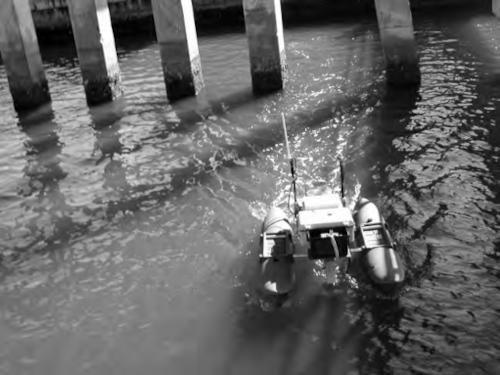
\includegraphics[width=\textwidth]{example1}
    \end{subfigure}
    \begin{subfigure}[b]{.325\textwidth}
        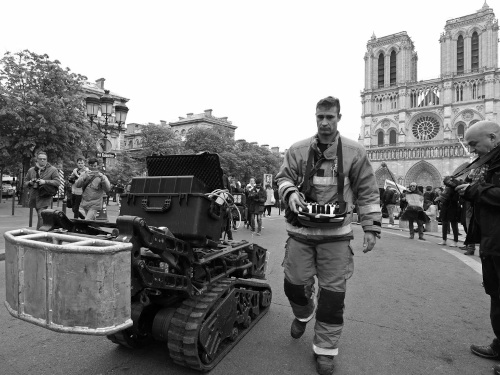
\includegraphics[width=\textwidth]{example2}
    \end{subfigure}
    \begin{subfigure}[b]{.325\textwidth}
        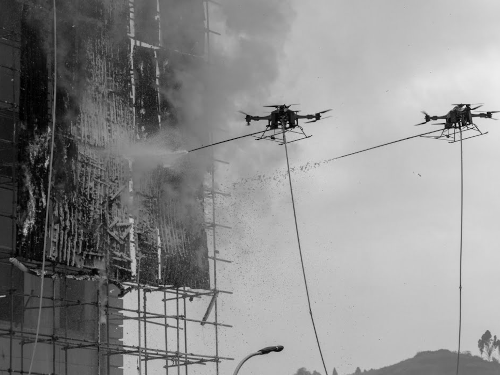
\includegraphics[width=\textwidth]{example3}
    \end{subfigure}
    \caption[Examples of cooperative coordination in disaster response]{%
    Examples of cooperative coordination in disaster response. From left to right: USV
    inspecting piers after Hurricane Wilma \cite{murphy2014}; the Colossus robot assisting
    the Paris Fire Brigade in the fight against the $2019$ Notre Dame Cathedral fire
    \cite{colossus}; fire-fighting UAVs in the Dazu District, China \cite{dazu}.}
\end{figure}

\iffalse
Oother motivating domains:
   - resource allocation (e.g., hospital workforce)
   - vehicle routing
   - combine harvesting
   - multi-factory scheduling
   - project scheduling
   - automated guided vehicles
   - open vehicle fleets
   - green maritime transportation
   - sensor networks
\fi

As can be seen, disaster response provides a comprehensive example of the various
challenges of cooperative coordination. In fact, it is a central class of case studies for
the multi-agent/robot systems community
\cite{rcr2001,murphy2014,dadvar2021,murphy2016a,murphy2016b}, as well as for AI in general
\cite{imran2014}. Based on this domain, we identify our problem below.

\section{Problem Statement}\label{sec:pstat}

We focus on the \emph{Coalition Formation with Spatial and Temporal constraints Problem}
(CFSTP) \cite{ramchurn2010cfstp}. We use the definitions of \emph{coalition} and
\emph{coalition formation} given by \cite{horling2005}. Hence, a coalition is a flat and
task-oriented organisation of agents, short-lived and disbanded when no longer needed,
while coalition formation is a consequence of the emergent behaviour of the system
\cite{mataric1993}.
Regardless of its current location, an agent is considered part of a coalition from the
moment it is assigned a task, to the moment the task is completed.
We consider coalitions to be different from teams (Figure \ref{fig:coalition-team}).
Moreover, based on \cite[Section $4.5$]{nunes2017taxonomy}, we consider a system to be
\emph{real-time} if it may have \emph{hard} deadlines, which cannot be violated, and
possibly also \emph{soft} deadlines, which can be violated with some penalty.
In the CFSTP, tasks (e.g., save victims or put out fires) have to be assigned to agents
(e.g., ambulances or fire brigades). The assignment is determined by the spatial
distribution of tasks in the disaster area, the time needed to reach them, the
workload they require (e.g., how large a fire is) and their deadlines (e.g., estimated
time left before victims perish). In addition to these constraints,
the number of agents may be much smaller than the number of tasks, hence they need to
cooperate with each other by forming, disbanding and reforming coalitions over time
\cite{shehory1998,epstein2011}.
The objective of the CFSTP is to define which tasks (e.g., sites with the most victims and
the strongest fires) to allocate to which coalitions (e.g., the fastest ambulances and
fire engines with the largest water tanks), in order to maximise the number of tasks
completed.
\begin{figure}[t]
    \centering
    \begin{subfigure}[b]{.49\textwidth}
        \centering
        \begin{tikzpicture}
    \node at (-0.25, 0.25) {\pgfuseplotmark{*}};
    \node at (-0.75, 0.5 ) {\pgfuseplotmark{*}};
    \node at (0.75 , 0.5 ) {\pgfuseplotmark{*}};
    \node at (0    , 0   ) {\pgfuseplotmark{*}};
    \node at (1    , 1   ) {\pgfuseplotmark{*}};
    \node at (-0.75, 1   ) {\pgfuseplotmark{*}};
    \node at (-1   , 1.5 ) {\pgfuseplotmark{*}};
    \node at (-0.25, 0.75) {\pgfuseplotmark{*}};
    \node at (0    , 2   ) {\pgfuseplotmark{*}};
    \node at (0.3  , 1.5 ) {\pgfuseplotmark{*}};
    \node at (0    , 0   ) {\pgfuseplotmark{*}};

    \draw (0, 1) circle (37pt);

    \node at (2.5 , -1.25) {\pgfuseplotmark{*}};
    \node at (2   , -1   ) {\pgfuseplotmark{*}};
    \node at (3   , -1   ) {\pgfuseplotmark{*}};
    \node at (1.75, -0.5 ) {\pgfuseplotmark{*}};
    \node at (2.5 ,  0   ) {\pgfuseplotmark{*}};
    \node at (2   ,  0.25) {\pgfuseplotmark{*}};
    \node at (2.9 , -0.6 ) {\pgfuseplotmark{*}};
    \node at (2.9 ,  0.4 ) {\pgfuseplotmark{*}};
    \node at (3.3 , -0.2 ) {\pgfuseplotmark{*}};

    \draw[densely dashdotted] (2.5, -0.35) circle (30pt);

    \node at (3   , 2    ) {\pgfuseplotmark{*}};
    \node at (3.2 , 2.7  ) {\pgfuseplotmark{*}};
    \node at (3.6 , 1.75 ) {\pgfuseplotmark{*}};
    \node at (2.5 , 1.5  ) {\pgfuseplotmark{*}};
    \node at (2.5 , 2.25 ) {\pgfuseplotmark{*}};
    \node at (3.25, 1.3  ) {\pgfuseplotmark{*}};

    \draw[dashed] (3, 2) circle (25pt);
\end{tikzpicture}

        \caption{Coalitions.}
    \end{subfigure}
    \hfill
    \begin{subfigure}[b]{.49\textwidth}
        \centering
        \raisebox{12pt}{
            \begin{adjustbox}{width=.9\textwidth}
                \begin{tikzpicture}
    \node (n1) at (0   , 0    ) {\pgfuseplotmark{*}};
    \node (n2) at (0.25, -1   ) {\pgfuseplotmark{*}};
    \node (n3) at (0.5 , -0.5 ) {\pgfuseplotmark{*}};
    \node (n4) at (-0.5, -0.75) {\pgfuseplotmark{*}};
    \node (n5) at (1   , -0.25) {\pgfuseplotmark{*}};
    \node (n6) at (1   , -1.25) {\pgfuseplotmark{*}};
    \node (n7) at (1.75, 0.25 ) {\pgfuseplotmark{*}};
    \node (n8) at (2.5 , 0    ) {\pgfuseplotmark{*}};
    \node (n9) at (2   , -0.75) {\pgfuseplotmark{*}};

    %\begin{scope}[-Straight Barb]
    \begin{scope}[-stealth]
    \draw (n1) -- (n2);
    \draw (n1) -- (n3);
    \draw (n1) -- (n4);
    \draw (n3) -- (n5);
    \draw (n5) -- (n7);
    \draw (n8) -- (n9);
    \end{scope}

    %\begin{scope}[Straight Barb-Straight Barb]
    \begin{scope}[stealth-stealth]
    \draw (n3) -- (n6);
    \draw (n7) -- (n8);
    \draw (n7) -- (n9);
    \end{scope}

    \draw (1, -0.45) ellipse (55pt and 1cm);
\end{tikzpicture}

            \end{adjustbox}}
        \caption{A team.}
    \end{subfigure}
    \caption[Differences between coalitions and teams]{%
        Differences between coalitions and teams \cite{horling2005}. Once formed, a
        coalition becomes an atomic entity that exists for a limited time, such
        as political parties joining together to form a government. In contrast, a team
        is a long-term organisation in which agents may have different roles, as in the
        game of football.}
    \label{fig:coalition-team}
\end{figure}

Despite having similarities with classic problems such as Generalised Assignment Problem
\cite{ross1975} and Job-Shop Problem \cite{brucker2007}, the importance of the CFSTP lies
in the fact that it was the first generalisation of the \emph{Team Orienteering Problem}
(TOP) to consider coalition formation \cite[Section $4.2$]{ramchurn2010cfstp}. For this
reason, it has been applied in contexts such as human-agent collectives
\cite{ramchurn2015a}, multi-UAV exploration \cite{baker2016}, and law enforcement
\cite{nelke2020,tkach2021}.

Within this problem class, our interest is in algorithms that are anytime (i.e., which can
return partial solutions if they are interrupted before completion), efficient, and have
theoretical properties. In other words, approximate algorithms \cite{papadimitriou1993}.
The reason is that they are fundamental in real-time domains, where it is necessary to
have provable guarantees, but it may be computationally not feasible or economically
undesirable to produce an optimal solution \cite{zilberstein1996,calvaresi2021}. In
particular, as we said above, the faster the disaster response, the lower the losses
incurred. We also assume that the agents are situated in a distributed system
\cite{tanenbaum2017} with a \emph{dynamic evolution of the environment}\footnote{Also
referred to as \emph{open} systems \cite{hewitt1990}. For brevity, we call them
\emph{dynamic environments}.} \cite{fioretto2018survey}, that is:
\begin{enumerate}
    \item It must be possible for agents to reach a solution through local interaction,
        rather than relying on a centralised solver \cite{ramchurn2010fms};
    \item At any time, agents can join in or leave, and new tasks can appear.
\end{enumerate}
If the problem is solved in a centralised fashion, then the designated solver has to be
informed whenever there is a change, recompute the solution, and redistribute it to all
agents.
In real-time domains such as disaster response, this leads to three major issues. First, a
centralised solver is a single point of failure that makes the system fragile and not
robust to unexpected events, such as malfunctions or communication disturbances between
agents far apart \cite{petcu2007thesis}. Second, if the agents have limited computational
resources and the problem is not small, electing a centralised solver might not be
possible, while distributing computations always improves scalability
\cite{tanenbaum2017}. Third, a centralised approach might not be as effective as a
distributed one, given that the situation can evolve rapidly and there could be
significant communication delays \cite{mailler2018}.

\section{Research Objectives and Methodology}\label{sec:objectives}

We aim to develop models, algorithms and test frameworks for multi-agent coordination,
with the following requirements.
\begin{description}[style=nextline]
    \item[R1] \emph{Decentralised autonomy}: the agents do not have to rely on a single
        point of failure. This is particularly important for disaster scenarios, where
        unreliable infrastructures and scarce supplies imply that lost resources cannot
        be replaced.
    \item[R2] \emph{Cooperation}: the agents have to coordinate their actions so to
        maximise their performance. Cooperation is also necessary when tasks require
        combined skills. For example, to extract survivors from the rubble of a collapsed
        building, rescue robots detect life signs with their sensors, firefighters dig and
        paramedics load the injured into ambulances.
        Therefore, the solutions must focus on achieving a global objective.
    \item[R3] \emph{Scalability}: the algorithms have to target scenarios with tens to
        thousands of agents and tasks, in order to be usable in future contexts where
        mass deployment of agents (e.g., robot swarms) will be common.
    \item[R4] \emph{Resilience}: agents and resources could be added and removed at any
        time, either by a human supervisor or due to unexpected failures. The algorithms
        must be able to produce feasible solutions even in such situations. If the
        solution quality degrades, it must happen in a controlled way.
\end{description}
Moreover, motivated by the disaster response domain, and intending to address the main
open issues in the MRTA literature \cite[Section $9.2$]{nunes2017taxonomy}, we make the
following assumptions.
\begin{description}[style=nextline]
    \item[A1] Tasks have spatio-temporal constraints (e.g., the buildings on fire are
        scattered throughout the city, and each will burn out completely after a certain
        amount of time). In particular, each task has a time window, with \emph{both} a
        soft and a hard deadline.
    \item[A2] There may be task precedences, such as when firefighters have to clear a
        road to allow ambulances to enter an area, and heterogeneous task weights, to
        capture situations in which some tasks may be more critical or urgent than others
        (e.g., saving lives has a greater benefit than clearing the rubble).
    \item[A3] Tasks may have multiple possible locations. This allows to characterise
        situations in which, for example, ambulances can transport the injured to
        different hospitals, or survivors can be transferred to various evacuation
        centres.
    \item[A4] Tasks require specific resources to be performed (e.g., it is estimated that
        the fire $x$ requires at least $y$ quantity of coolant to be extinguished).
    \item[A5] The environment is dynamic. For instance, at any moment, new fires could
        break out, or other buildings could collapse, hence first responders must be ready
        to deploy to other areas.
\end{description}

According to \cite{fioretto2018survey}, to date the main disciplines that have been used
for solving cooperative coordination problems are game theory
\cite{myerson1997,osborne1994}, decision theory \cite{keeney1993} and constraint
programming \cite{dechter2003,rossi2006handbook}.

Usually, cooperative game theory models do not have a distributed design\footnote{Rather,
there are models that combine non-cooperative game theory with distributed constraint
optimisation \cite{chapman2010,chapman2011,chapman2011b,zou2021}.}, or are based on the
impractical assumption that calculations have no cost. On the other hand, decision theory
is afflicted by super-polynomial complexity \cite{bellman2003}, thus designing scalable
algorithms (Requirement R3) imposes additional assumptions that may be too limiting for
realistic scenarios \cite{diederich2001,cerquides2013}.

Hence, we choose to work with constraint programming, which, as we will show in the
following chapters, allows us to meet all our research objectives. In Chapter
\ref{chap:lit}, we review each of the above approaches and give a thorough motivation of
our choice.

\section{Research Contributions}\label{sec:contrib}

We start with an in-depth analysis of \emph{Coalition Formation with Look-Ahead} (CFLA),
the state-of-the-art CFSTP algorithm. We outline two main limitations. First, its time
complexity is exponential in the number of agents. Second, as we show, its look-ahead
technique is not effective in real-world scenarios, such as dynamic environments, where
new tasks can appear at any time. To achieve better performance, we define an extension
called CFLA2. However, since we cannot eliminate the design limitations of CFLA in CFLA2,
we also develop a novel algorithm called \emph{Cluster-based Task Scheduling} (CTS), the
first to be simultaneously anytime, efficient and with convergence guarantee. We
empirically show that, in settings where the look-ahead technique is highly effective, CTS
completes up to $30\%$ (resp. $10\%$) more tasks than CFLA (resp. CFLA2), while being up
to four orders of magnitude faster. We also propose S-CTS, a simplified but parallel and
more efficient variant of CTS. In problems generated by the RoboCup Rescue Simulation
\cite{rcr2001}, S-CTS is at most $10\%$ less performing than high-performance algorithms
such as Binary Max-Sum \cite{pujol-gonzalez2014binary} and DSA \cite{zhang2005}, but up to
two orders of magnitude faster.

We then go on to identify the main issues in the CFSTP literature, namely, its original
mathematical programming formulation, which is lengthy and difficult to implement, and the
lack of a distributed, dynamic and scalable algorithm. Consequently, we propose a minimal
mathematical program, and reduce the CFSTP to a \emph{Dynamic and Distributed Constraint
Optimisation Problem} (DynDCOP) \cite{fioretto2018survey}, on which we design D-CTS, a
distributed version of CTS. Using public London Fire Brigade records
\cite{lfb-incident,lfb-mobilisation}, we create a large dataset and a test framework that
simulates the mobilisation of firefighters in dynamic environments. In problems with up to
$150$ agents and $3000$ tasks, compared to DSA-SDP, a state-of-the-art distributed
algorithm \cite{zivan2014}, D-CTS completes approximately the same percentage of tasks,
but with the advantage of being one order of magnitude more efficient in terms of
communication overhead and time complexity.

Finally, to characterise scenarios in which the faster the tasks are solved, the greater
the benefits, we propose the \emph{Multi-Agent Routing and Scheduling through Coalition
Formation problem} (MARSC), a generalisation of both the CFSTP and the important
\emph{Team Orienteering Problem with Time Windows} (TOPTW) \cite{top2019}. We formulate a
binary integer program \cite{wolsey2020} and propose \emph{Anytime, exact and parallel
Node Traversal} (ANT), the first MARSC algorithm of its kind, which is also the first
exact CFSTP algorithm. Moreover, we define an approximate variant called
ANT-$\varepsilon$.
On a machine with RHEL $7.9$ operating system, a $2$ GHz CPU with $40$ threads, and $24$
GB of DDR4-$2666$ SDRAM, ANT can find optimal solutions to problems with $2$ agents and up
to $40$ tasks in less than $25$ minutes. With the same operating system and CPU, but with
$187.5$ GB RAM, the industry-leading CPLEX solver version $20.1$ runs out of memory and
crashes. On the other hand, in problems with $150$ agents and up to $3000$ tasks,
ANT-$\varepsilon$ finds $2.6$ times better median solutions and is $3.65$ times faster
than an extended version of CTS.

Since the MARSC generalises or can be reduced to important combinatorial
optimisation problems (Figure \ref{fig:relationships}), our results can also be applied to
widely studied sub-problems such as the TOPTW, and be adapted to domains that are similar
to or less challenging than disaster response, such as those mentioned at the beginning of
this chapter (Page \pageref{chap:intro}).

Our work has produced the following articles.
\clearpage

\begin{figure}[t]
    \centering
    \begin{adjustbox}{width=.7\textwidth}
        \begin{tikzpicture}
    \begin{scope}%[set style={{every node}=[draw]}]
        \node (cfstp) at (0,  0) {CFSTP};
        \node (marsc) at (4,  0) {\textbf{MARSC}};
        \node (ddcop) at (8,  0) {DynDCOP};
        \node (top)   at (0, -2) {TOP};
        \node (toptw) at (4, -2) {TOPTW};
        \node (dcop)  at (8, -2) {DCOP};
        \node (vrpp)  at (0, -4) {VRPP};
        \node (vrp)   at (4, -4) {VRP};
        \node (tsp)   at (8, -4) {TSP};
    \end{scope}
    \begin{scope}[-{Triangle[open]}] % generalisation
        \draw (tsp)   -- (vrp);
        \draw (vrp)   -- (vrpp);
        \draw (top)   -- (toptw);
        \draw (top)   -- (cfstp);
        \draw (toptw) -- (marsc);
        \draw (cfstp) -- (marsc);
        \draw (dcop)  -- (ddcop);
    \end{scope}
    \begin{scope}[Straight Barb-] % association
        \draw (vrpp)  -- (top)   node[fill=white, outer sep=0, pos=0.5] {\small variant of};
        \draw (ddcop) -- (marsc) node[pos=0.5, above, sloped] {\small reduced to};
    \end{scope}
\end{tikzpicture}

    \end{adjustbox}
    \caption[Class diagram of the problems considered]{Class diagram of the
    relationships between the combinatorial optimisation problems that we consider.
    We generalise the CFSTP into the MARSC, and show how both can be reduced
    to a DynDCOP, an extension of the DCOP \cite{fioretto2018survey}. We also show
    that the MARSC generalises the TOPTW, an extension of the TOP, the latter
    generalised by the CFSTP (Section \ref{sec:pstat}). The TOP is a variant of the
    \emph{Vehicle Routing Problem with Profits} (VRPP), which generalises the
    \emph{Vehicle Routing Problem} (VRP) and the \emph{Travelling Salesman
    Problem} (TSP) \cite{top2019}.}
    \label{fig:relationships}
\end{figure}

\begin{enumerate}
    \item Capezzuto, Luca, Danesh Tarapore, and Sarvapali D. Ramchurn.
        \emph{Anytime and Efficient Coalition Formation with Spatial and Temporal
        Constraints}. EUMAS-AT 2020: Multi-Agent Systems and Agreement Technologies, pp.
        $589 - 606$ (2020). Springer, Cham.
    \item Capezzuto, Luca, Danesh Tarapore, and Sarvapali D. Ramchurn.
        \emph{Anytime and Efficient Multi-agent Coordination for Disaster Response}. SN
        Computer Science 2.3, pp. $1 - 15$ (2021).
    \item Capezzuto, Luca, Danesh Tarapore, and Sarvapali D. Ramchurn.
        \emph{Multi-Agent Routing and Scheduling through Coalition Formation}. 12th
        Workshop on Optimisation and Learning in Multi-Agent Systems (OptLearnMAS), held
        at the 20th International Conference on Autonomous Agents and Multiagent Systems
        (AAMAS 2021).
    \item Capezzuto, Luca, Danesh Tarapore, and Sarvapali D. Ramchurn.
        \emph{Large-scale, Dynamic and Distributed Coalition Formation with Spatial and
        Temporal Constraints}. 18th European Conference on Multi-Agent Systems (EUMAS
        2021), Revised Selected Papers, pp. $108 - 125$ (2021). Springer, Cham.
\end{enumerate}

Chapter \ref{chap:contrib1} is composed of Articles $1$ and $2$, Chapter
\ref{chap:contrib2} is Article $4$ with minor exposition improvements, while Chapter
\ref{chap:contrib3} is an extension of Article $3$.

\section{Thesis Outline}\label{sec:outline}

The remaining chapters are structured as follows.

\paragraph{Chapter \ref{chap:lit}}
A survey of multi-agent coalition formation for task allocation in the research fields
identified in Section \ref{sec:objectives}.
Its has two purposes. First, it motivates in detail which field we choose to work with.
Second, it shows that, although many existing models come close to our objectives, no one
can satisfy them all, which motivates the proposal of the MARSC in Chapter
\ref{chap:contrib3}.

\paragraph{Chapter \ref{chap:background}}
The topics on which the following chapters will be based: our constraint programming
formulation of the CFSTP; the CFLA algorithm, and the original mixed integer programming
formulation of the CFSTP.

\paragraph{Chapter \ref{chap:contrib1}}
The CFLA2 algorithm, a novel variant of CFLA. Design of the CTS algorithm, the new
state-of-the-art CFSTP algorithm. Definition of the parallel variant S-CTS, and empirical
evaluation with the RoboCup Rescue Simulation against the high-performance Binary Max-Sum
and DSA algorithms.
%\clearpage

\paragraph{Chapter \ref{chap:contrib2}}
A minimal binary integer program of the CFSTP, and a reduction to the DynDCOP formalism.
Design of D-CTS, a distributed version of CTS, and empirical evaluation on our large-scale
and realistic test framework based on London Fire Brigade records.

\paragraph{Chapter \ref{chap:contrib3}}
Formulation of the MARSC, a generalisation of the CFSTP and the TOPTW that can be used in
real-time domains. Design of ANT, the first anytime, exact and parallel MARSC algorithm,
as well as the approximate variant ANT-$\varepsilon$.

\paragraph{\nameref{chap:conclusions}}
Summary of the strengths and limitations of our work, followed by a list of possible
directions for future work.

\chapter{Literature Review}\label{chap:lit}

This chapter reviews the areas identified in Section \ref{sec:objectives}, namely, game
theory, decision theory and constraint programming. Based on the classifications of
\cite{ye2016,cerquides2013,cao2013,farinelli2004,ponda2015,
korsah2013taxonomy,gini2017,nunes2017taxonomy,khamis2015,parker2016,jahn2020,miloradovic2019tamer,skaltsis2021survey,verma2021,aziz2021},
we identify $3$ fundamental approaches to cooperative coordination: coalition formation in
game theory (Section \ref{sec:cf}); Markov decision processes in decision
theory\footnote{More precisely, in the subfield of multi-agent planning
\cite{torreno2017}.} (Section \ref{sec:mdp}), and distributed constraint optimisation
problems in constraint programming (Section \ref{sec:dcop0}).

For each approach, we highlight the main results that are relevant to our
objectives (Section \ref{sec:objectives}). Then, in Section \ref{chap2:choice}, we explain
which approach we choose to work with in the following chapters.
Finally, in Section \ref{chap2:limitations}, we list the limitations of our starting model
(Section \ref{sec:pstat}) in relation to our objectives, and show that no work proposed so
far is able to address all of them. This motivates the introduction of the novel model in
Chapter \ref{chap:contrib3}.

\section{Coalition Formation}\label{sec:cf}

Task allocation through \emph{Coalition Formation} (CF) models scenarios where tasks
cannot be performed by a single agent \cite{shehory1998}. It consists of $3$
phases \cite{sandholm1999}:
\begin{enumerate}
    \item \gls{csg}: partitioning of agents into exhaustive and disjoint sets such that
        only agents within the same set cooperate. Such sets are called \emph{coalitions},
        while the partition is called \emph{coalition structure};
    \item \emph{Coalition value calculation}: for each coalition $C$, definition of a
        measure of the expected outcome that could be derived if $C$ was formed. Once the
        calculation is done, the decision about how to optimally form coalitions can be
        taken, which depends on the given problem;
    \item \emph{Revenue distribution}: determination of the rewards for each agent in
        order to get \emph{stable} coalitions \cite{rahwan2009}. A coalition is stable if
        its agents have no incentive to deviate from it. This property is also known as
        \emph{incentive compatibility} \cite[Section $9.3.2$]{nisan2007}.
\end{enumerate}
The most important phase is that of CSG, since the number of possible coalition structures
is exponential in the number of agents. Specifically, the time complexity required
to find an optimal coalition structure is $O(a^a)$ and $\omega(a^{a/2})$, where
$a$ is the number of agents. Furthermore, the problem is NP-complete \cite{sandholm1999}.
For this reason, a wide range of approximate algorithms has been developed so far, using
approaches from mathematical programming, stochastic search and machine learning. In the
remainder of this section, we will review some important works that are of interest to our
context. We refer to \cite{rahwan2015survey} for a thorough survey on CSG.

Among the first and best-known attempts to study algorithmic aspects of CSG, we find
\cite{shehory1998}. They developed decentralised, anytime and dynamic algorithms with low
ratio bounds and low computational complexity, where coalitions may have a precedence
order. Their limitation is the assumption that coalition resources can be transferred
between agents, which reduces the solution space.

An optimal solution to the CSG problem has been given by \cite{rahwan2009}. They represent
the solution space through integer partition \cite{andrews2004} and solve the problem
using a branch-and-bound technique. The limitation of this approach is that, in the worst
case, the number of coalition structures to be searched is intractable. As a result, the
algorithm is not scalable (Requirement R3).

A CF model with incomplete information, limited computational resources, and time
constraints was proposed by \cite{kraus2003,kraus2004}. Their mechanism consists of an
auction protocol and $2$ heuristic algorithms. Experimental results show that their
algorithms are stable and increase social welfare, compared to previous strategies. There
are $2$ limitations in the work. First, it focuses specifically on the Request For
Proposal domain, where the tasks are independent. Therefore, it cannot be
used in settings where there may be task precedences (Assumption A2). Second, the
algorithms have no theoretical guarantees, while we aim at approximate algorithms (Section
\ref{sec:objectives}).

A variant of CSG is the \emph{Graph-Constrained Coalition Formation} (GCCF)
\cite{myerson1977}, where agents have a graph of relationships $G$ and a coalition $C$ is
considered feasible if all agents in $C$ are connected by a subgraph of $G$ induced by
$C$. This formulation allows solving a wide range of real-world problems. An interesting
one is the Social Ridesharing problem \cite{bistaffa2015}, in which a community of
commuters (e.g., riders and drivers) need to form coalitions (e.g., joining in cars) while
meeting the constraints imposed by the social network (e.g., users prefer to ride with
friends). The objective is to minimise associated transportation costs, like travel time
and fuel. The model has been extended to also allow temporal constraints, such as desired
pick-up and arriving times \cite{bistaffa2017a}. For a survey on real-world GCCF
applications, we refer to \cite{bistaffa2017b}. Such approaches can cope with
spatio-temporal and resource constraints (Assumptions A1 and A4). Nonetheless, they are
offline, which implies that situations where agents can join in or leave cannot be
considered (Requirement R4 and Assumption A5). \cite{flammini2018} have proposed an online
GCCF model in which the graph is weighted and agents are assigned to coalitions
irrevocably. However, their model cannot solve problems where the graph is unweighted or
coalitions can be modified (Requirement R4).

Another variant of CSG is the \emph{Overlapping Coalition Formation} (OCF) model
\cite{chalkiadakis2010}, where agents may be involved in more than one task and thus may
distribute their resources among multiple coalitions. There is no inherent superadditivity
assumption, therefore it is possible to capture scenarios in which not always any pair of
coalitions is best off by merging into one\footnote{That is, scenarios in which the
emergence of the \emph{grand coalition}, or the coalition of all agents, is either not
guaranteed or impossible \cite{sandholm1997,sandholm1999}.}. To date, however, there
is still no characterisation of scenarios where overlapping coalitions can naturally
arise (Assumption A5). \cite{zick2012} showed that the OCF can be reduced to the
Unbounded Knapsack Problem \cite{martello1990}, thus proving that it is NP-complete.
They also identified that the computational complexity depends on the amount of
resources possessed by each agent, the maximum coalition size, and the pattern of
interaction among agents. Furthermore, they proposed tractable subproblems with
discrete resources and limited interactions.

\cite{rahwan2013coalitional} proposed the \emph{Coalition-Flow Network} (CF-NET) model,
where a characteristic function game can be represented as a network flow problem. In the
CF-NET model, the value of a coalition is associated with both the execution of a given
task and the types of the agents involved. Agents can participate in multiple coalitions
simultaneously, which allows to consider both CSG and OCF problems. In addition, each agent
has a limit on the resources that can use to execute tasks, thus there is an upper bound
on the number of coalitions it can join. An anytime approximate algorithm is proposed,
which provides worst-case guarantees on the solution quality. Although it permits to
switch between cases with non-overlapping and overlapping coalitions efficiently, with and
without agent types, the work does not consider scenarios where the order in
which agents join a coalition can affect the value of the coalition \cite{michalak2014}.
Hence, it is not suitable for real-time domains such as disaster response.

A typical assumption in CF is that the values of potential coalitions are known with
certainty, and agents have complete information on the capabilities of potential partners.
\cite{chalkiadakis2004,chalkiadakis2012} have proposed a model in which both coalition
values and agent capabilities are uncertain, and Bayesian \emph{Reinforcement Learning}
(RL) \cite{brl2015survey} is used to reduce such uncertainties. The rationale for using RL
is that agents are supposed to interact between each other by repeatedly exchanging
messages, therefore the more they interact, the more accurate their beliefs about each
other's capabilities.
Their stability criterion, called \emph{Bayesian core}, makes agent $a$ choose coalition
$C$ based not only on the value of $C$, but also on its \emph{value of information},
defined as the quantity of information that $a$ can learn about other agents if $C$ was
formed. Since the proposed inferential process does not consider the cost of computation,
it is not clear how the model can handle large-scale problems (Requirement R3). Another
limitation is that RL approaches, and machine learning in general\footnote{Not considering
open problems such as brittleness, embedded bias, catastrophic forgetting, and
explainability \cite{ml-failures,dehghani2021,roy2021}, as well as the non-trivial
requirement to adjust parameters according to available data and target application
\cite{vasudevan2021}. In fact, in industry it is good practice to start without machine
learning \cite{yan2021}.}, are inapplicable to our domains of interest due to their
initial training phase: before they can generate feasible solutions, the problem
formulation may change, thus new training may become necessary \cite{tsimenidis2020}.
Moreover, such approaches are notoriously sample-inefficient, that is, they usually need
millions of interactions even for the simplest problems \cite{yang2021survey}. This
latency is particularly undesirable in real-time scenarios, where the situation can evolve
quickly (Assumption A3).

\cite{krausburg2021} introduced the \emph{Sequential Characteristic Function Game} (SCFG),
which extends the CSG problem to a total order of structures defined by binary relations.
A variant of the clustering heuristic by \cite{farinelli2017} is proposed to solve the
problem, and $2$ examples show that the model is able to characterise disaster response
scenarios where agents can be organised in dynamic hierarchies of coalitions to respond to
various events. Although it opens up new research directions in game theoretic CF, the
SCFG is only able to meet our Assumptions A2 and A5.

\cite{czarnecki2021} use a maximum bipartite graph matching and a hedonic CSG
\cite{bogomolnaia2002} to address MRTA domains that require to minimise formation costs
and to maximise coalition values. Their approach is guaranteed to reach a Nash
equilibrium, and capable to solve problems with thousands of robots and hundreds of tasks
in seconds, which satisfies Requirement R3. However, it does not take any of our remaining
objectives into account.

\section{Markov Decision Processes}\label{sec:mdp}

\emph{Markov Decision Processes} (MDPs) \cite{seuken2008} are widely used in cooperative
coordination \cite{torreno2017}, given their capability to model stochastic and sequential
decision making \cite{sutton1998,diederich2001,kolobov2012}, and have been successfully
applied to many agent-based models, multi-agent systems and multi-robot systems.
\cite{smith1981,stone2005,guestrin2002,denijs2021,kurniawati2021survey}.
Since their computational complexity is super-polynomial in the number of agents
\cite{bellman2003}, MDP algorithms are typically approximate
\cite{sutton1996,bertsekas2012,mahadevan2007,busoniu2017,geramifard2011}.

In the standard MDP model, agents are able at every time step to observe the whole global
state. This is not possible in presence of uncertainty, where agents can only infer
information on the global state by observing the environment. The \gls{pomdp} model
extends the MDP model to such domains \cite{seuken2008}. Solving POMDPs is much more
computationally expensive than solving MDPs, because the optimal policy is a mapping from
a belief space (over the state space) to the action space, rather than from the state
space to the action space. Thus, the problem dimension is exponentially increased.

When the MDP and POMDP models are applied to multi-agent scenarios, the resulting models
are called \emph{Multi-agent (Partially Observable) Markov Decision Processes} (MMDP and
MPOMDP, respectively). The main difference is that decisions are collective, therefore
there are: a \emph{joint} agent state space; a \emph{joint} action space, and a
\emph{joint} observation space. It is demonstrated that the computational complexity of
M(PO)MDPs is exponential in the number of agents \cite{redding2012}. Furthermore,
a limiting assumption of these models is that each agent is required to have a \emph{full}
(MMDPs) or \emph{partial} (MPOMDPs) \emph{individual observability} of the global state.
That is, each agent must have the same full or partial knowledge of the joint state.

When agents decide and observe locally, the assumption of individual observability is in
general impractical, as it requires that every agent communicate its observations to
every other agent at every time step, with no communication costs. This is typically
referred to as a \emph{free-comm} environment \cite{ponda2015}. However, in real-world
situations like disaster response, communication might have operational constraints, such
as limited bandwidth or network topology. To address this issue, various decentralised
(PO)MDP variants have been proposed, but they further increase the problem dimension
and thus worsen the computational complexity. The \emph{Decentralised MDP} (Dec-MDP)
model, first proposed by \cite{bernstein2002}, replaces the assumption of full
individual observability with a full joint observability requirement: the sum of all agent
observations must be equal to the full observability of the global state. To do so, agents
share their observations through communication. However, this overhead has NEXPTIME
complexity. If the global state cannot be uniquely determined by a joint observation, the
Dec-MDP becomes a Dec-POMDP \cite{bernstein2002}. The Dec-POMDP has been proven to be
equivalent to the \emph{Multi-agent Team Decision Problem} (MTDP) \cite{pynadath2002} in
terms of computational complexity and expressiveness of representation \cite{seuken2008}.
If a free-comm environment is assumed, then Dec-MDP and Dec-POMDP reduce to MMDP and
MPOMDP, respectively \cite{goldman2004}.

Since the communication infrastructure plays a key role in decentralised architectures,
the above models have also been extended to capture agent communication protocols. The
resulting variants, namely the Dec-POMDP-COM \cite{goldman2003} and the COM-MTDP
\cite{pynadath2002}, define communications as actions on which agents must make explicit
decisions. In other words, sending a message is also an action with an associated cost,
and every agent has to decide which messages to send at each time step, where the decision
not to send a message is modelled as a null message with zero cost. It is shown that
Dec-POMDP, MTDP, Dec-POMDP-COM and COM-MTDP are all NEXPTIME-complete in the number of
agents \cite{seuken2008}.

In MDP models, the complexity of a problem is directly linked to the assumptions on
observability and communication \cite{seuken2008}. To keep the computational complexity
tractable, the problem is typically relaxed. Among the most interesting approximate
MDP model, we find the \emph{Transition Independent Dec-MDP} (TI-Dec-MDP)
\cite{becker2004}, where agents are independent and collaborate with each other through a
global reward function of all agent states and actions. The TI-Dec-MDP extends
a factored version of Dec-MDP, in which the global state is divided into
$2$ parts: information about local agent states, and information about the environmental
variables of interest. In this model, the dynamics that rule the state transitions and
observations of each agent are independent (i.e., they are functions only of the local
agent and the world state), and agents are only coupled through the global reward
function. Being based on independent agents, the TI-Dec-MDP scales in time better than
other models, but it is also more space demanding, because it requires that each agent
stores its complete state transition history \cite{becker2004,redding2012}. Moreover, the
independence assumption does not allow to explicitly model situations due to combinations
of agent states (e.g., UAV collisions), even though these can be defined by assigning very
large negative rewards (e.g., instead of being defined as a set of constraints, collision
avoidance could be integrated into the global reward function). Other notable approximate
models include:
\begin{itemize}
    \item The decentralised sparse-interaction MDP \cite{melo2011}, in which the agent
        state space is subdivided into $2$ subsets: states where agents need to cooperate,
        and states where they can act independently;
    \item The group-aggregate Dec-MMDP \cite{redding2012}, where each agent stores only
        some properties of interest regarding other agent state-action spaces (e.g., the
        number of agents in a particular area, or the location of a particular subset of
        agents);
    \item The auctioned POMDP \cite{capitan2013}, in which agents solve their local
        version of the global problem (optimised to their preferences), then negotiate a
        global solution through an auction protocol;
    \item The POMDP with information rewards \cite{spaan2015}, where agents are
        rewarded for reaching certain levels of belief on target state features. This
        model is designed for robot-assisted surveillance, where robots have to take into
        account the influence of actions on the environment, as well as the potential
        information gain;
    \item The POMDP with macro-actions \cite{amato2016}, aimed at solving MRTA
        allocation problems. A \emph{macro-action} is a set of actions necessary to
        complete a high-level goal, and includes low-level actions such as moving,
        manipulating, and perception. \cite{smith2019} extended the framework using
        \emph{Monte Carlo Tree Search} (MCTS) to search the action spaces and allow
        real-time planning;
    \item The mixed observed MDP \cite{chen2021}, combined with a factor graph formulation
        and solved with the decentralised Max-Sum algorithm (Section \ref{sec:dcop}).
\end{itemize}
Summing up, computational complexity in MDPs can be reduced through approximate
techniques, but this yields to problem-dependent solutions. Concerning disaster response
problems, important models and solution techniques are listed below:
\begin{itemize}
    \item Multi-agent POMDP with online Bayesian learning \cite{allen2010}, in which agent
        policies are defined through deterministic finite state machines built with
        Bayesian learning. Heuristics specific to search and rescue problems are used to
        estimate the values of future states to add;
    \item Multi-agent POMDP with MCTS \cite{amato2015}, which extends the seminal online
        planning method by \cite{silver2010} to multi-agent planning and learning
        domains, with particular interest in fire-fighting and sensor network problems
        with up to $10$ agents.
    \item Multi-agent MDP with MCTS \cite{ramchurn2015a}. The considered problem is the
        CFSTP \cite{ramchurn2010cfstp}, extended to capture the uncertainties of a threat
        diffusing in an aftermath area (e.g., a radioactive cloud), and the activity of
        first responders. To cope with dimensionality issues, an approximate algorithm is
        developed using MCTS to estimate the expected value of teams. Under the same
        settings, \cite{baker2016} proposed a decentralised variant of MCTS that allows
        coordinating multiple UAVs in the exploration of continuous disaster spaces, with
        the aim of maximising the probability of discovering survivors;
    \item Multi-agent MDP with rejections, called $k$-RMMDP \cite{ramchurn2016}, which
        is based on the probability that a set of agents $T_H$ rejects a joint action in a
        given state, while each other agent $\notin T_H$ accepts it. A novel approach,
        called \emph{Two-Pass Planning} (TPP), is proposed to solve $k$-RMMDPs ad hoc.
        Empirical evaluation shows that, in human-\emph{in}-the-loop settings, TTP task
        allocations are more likely to be accepted by first responders, and also have a
        better completion rate with respect to human-\emph{on}-the-loop settings;
    \item POMDP with online planning and active sensing \cite{wu2016}, where Monte Carlo
        simulation (for one human) is combined with information-based active sensing (for
        multiple UAVs) using an anytime heuristic;
    \item Qualitative Dec-POMDP (QDec-POMDP) with iterative planning \cite{bazinin2018}.
        A QDec-POMDP is a Dec-POMDP in which the quantitative probability distributions
        over state spaces are replaced with qualitative sets of states. Although this
        change improves the scalability, it does not alter the computational complexity;
    \item Dec-POMDP with multi-agent reinforcement learning \cite{lee2021} pre-trained by
        behavioural cloning \cite{lee2021} to solve selective patient admission
        problems, in which an emergency department strategically reassigns some of the
        incoming patients to other emergency departments to preserve its medical resources
        for future severe patients.
\end{itemize}
None of the solutions presented above meets all of our requirements (Section
\ref{sec:objectives}), because they are either based on heuristics
\cite{allen2010,baker2016,wu2016,bazinin2018} (we aim at solutions with provable
guarantees), or rely on a centralised solver \cite{amato2015,ramchurn2015a,ramchurn2016}
(Requirement R1 impose decentralised solutions), or are not usable in dynamic environments
\cite{lee2021} (Assumption A5).

\section{Distributed Constraint Optimisation Problems}\label{sec:dcop0}

A generalisation of the Distributed Constraint Satisfaction Problem
\cite{yokoo1998}, the \emph{Distributed Constraint Optimisation Problem}
(DCOP)\footnote{Originally abbreviated to \emph{DisCOP} \cite{meisels2007}.}
\cite{farinelli2013dcop} can be classified according to the following parameters
\cite{fioretto2018survey}:
\begin{itemize}
    \item \emph{Agent behaviour}: how agents act. It can be deterministic or stochastic;
    \item \emph{Agent knowledge}: how much agents know about their state and the state of
        the environment. It can be total or partial;
    \item \emph{Agent coordination}: how agents interact. It can be cooperative (common
        goals) or competitive (individual goals);
    \item \emph{Environment behaviour}: how the environment reacts to the execution of an
        action. It can be deterministic or stochastic;
    \item \emph{Environment evolution}: this parameter defines whether the problem changes
        over time (dynamic) or not (static).
\end{itemize}

\begin{table}[t]
    \centering
    \begin{tabular}{lcc}
        \toprule
        EE / EB &
        \textsc{Deterministic} & \textsc{Stochastic}\\
        \midrule
        \textsc{Static} & DCOP & Probabilistic DCOP\\
        \midrule
        \textsc{Dynamic} & Dynamic DCOP & --\\
        \bottomrule
    \end{tabular}
    \caption[DCOP model taxonomy]{DCOP models \cite{fioretto2018survey}. The columns refer
    to the environment evolution (EE), while the rows refer to the environment behaviour
    (EB). In this thesis, we focus on the first column.}
    \label{t:dcop}
\end{table}

Table \ref{t:dcop} lists the models associated with this classification. The DCOP is a
direct extension to distributed environments of the \gls{cop}. It is characterised by
static and deterministic environment, deterministic agent behaviour, total agent
knowledge, and cooperative agent coordination. \emph{Dynamic DCOPs} (DynDCOPs) are based on
decision theory concepts to model dynamic environments.
Given our objectives (Section \ref{sec:objectives}), in the next sections we give a formal
definition of DCOPs and DynDCOPs, along with a summary of state-of-the-art algorithms.
Following \cite[Section $4.3$]{fioretto2018survey}, we will use the term \emph{incomplete}
to denote an algorithm that is either approximate or heuristic (i.e., not exact).

\subsection{DCOP}\label{sec:dcop}

Following \cite[Section $2.1$]{petcu2007thesis}, we begin by formulating the centralised
and discrete COP.
\begin{definition}\label{def:cop}
    A COP is a tuple $\mathcal{P} = \langle X, D, R \rangle$, where $X$ is a set of $n$
    variables, $X = \{x_1, \dots, x_n\}$, $D$ is a corresponding set of finite domains, $D
    = \{D_1, \dots, D_n\}$ such that $x_i \in D_i$, and R is a set of $t$ cost functions,
    $R = \{r_1, \dots, r_t\}$, with $r_i : D_{i_1} \times \cdots \times r_{i_h} \to
    \mathbb{R}$, $1 \leq i \leq t$, $h \leq n$.
    An assignment to $\mathcal{P}$ is a set of $k$ values $d = \{d_1, \dots, d_k \}$, $k
    \leq n$, where $d_i \in D_i$. If $k < n$, $d$ is called \emph{partial assignment}, and
    \emph{complete assignment} otherwise. An optimal solution to $\mathcal{P}$ is a
    complete assignment $X^\ast$ that minimises the sum of all costs:
    \begin{equation}
        X^\ast = \arg \min_{\substack{d \in D\\ |d| = n}} \sum_{r_i \in R} r_i(d)
    \end{equation}
\end{definition}
In the previous definition, the functions in $R$ are soft constraints. Nonetheless, hard
constraints can be imposed by defining cost functions that evaluate feasible assignments
to $0$, and unfeasible ones to $+\infty$. The discrete DCOP can be formulated as follows.
\begin{definition}\label{def:dcop}
    A DCOP is a tuple $\mathcal{P} = \langle A, P, R^{ia} \rangle$ such that:
    \begin{itemize}
        \item $A$ is a set of $m$ agents, $A = \{ A_1, \dots, A_m \}$;
        \item $P = \{\mathcal{COP}_1, \dots, \mathcal{COP}_k\}$ is a set of disjoint COPs
            (definition \ref{def:cop});
        \item Each $\mathcal{COP}_i \in P$ is called the \emph{local subproblem} of agent
            $A_i$, who owns and controls it;
        \item $R^{ia} = \{ r_1, \dots, r_t \}$ is a set of \emph{inter-agent} cost
            functions defined over variables from multiple local subproblems. In
            particular, each $r_i \in R$ expresses the value of all possible joint
            decisions that can be made by the agents that control the local subproblems
            involved in $r_i$. The agents involved in $r_i$ have full knowledge of $r_i$
            and are called \emph{responsible} for $r_i$.
    \end{itemize}
    An optimal solution to $\mathcal{P}$ is a complete assignment to all variables of all
    local subproblems, such that the sum of all inter-agent cost functions is minimised.
\end{definition}
Thus, a DCOP is a multi-agent system in which each agent controls its local COP. Hard
constraints can be imposed in DCOPs with the procedure described above for COPs. It is
commonly assumed that every cost function is known to all involved agents.
The DCOP is NP-hard \cite{farinelli2013dcop}.
A typical data structure for representing a DCOP is the factor graph
\cite{kschischang2001,loeliger2004}.
\begin{definition}\label{def:fg}
    A \emph{factor graph} is a bipartite graph expressing the factors of a function. The
    factor graph of a DCOP $\mathcal{P}$ is composed of:
    \begin{itemize}
        \item \emph{Variable nodes}, representing the COP variables in $\mathcal{P}$;
        \item \emph{Factor nodes}, representing all COP constraints and inter-agent
            constraints in $\mathcal{P}$;
        \item Undirected edges between each factor node and the variable nodes in its
            scope.
    \end{itemize}
\end{definition}
Other data structures to represent DCOPs are constraint graphs and pseudo-tree
\cite{fioretto2018survey}. A \emph{constraint graph} is an undirected
hypergraph\footnote{A generalisation of a graph in which an edge can join $2$ or more
vertices.} where nodes represent the decision variables, and edges represent the
constraints. Two nodes are in the same edge if the respective variables occur in the same
constraint \cite{rossi2006handbook}. A \emph{pseudo-tree} is a connected pseudo-forest,
that is, an undirected connected graph that contains at most one cycle\footnote{Connected
acyclic graphs (trees) are therefore pseudo-trees.}.
Constraint graphs allow to define priorities between variables, and pseudo-trees capture
partial orders among the agents.

Depending on how decision variables are updated, DCOP algorithms are divided into
synchronous and asynchronous. \emph{Synchronous} algorithms impose an order on how agents
make their decisions, typically through the data structure used for representation. In
contrast, \emph{asynchronous} algorithms allow agents to make their decisions based
uniquely on their local views of the problem. Synchronous algorithms introduce
dependencies between agents, but guarantee that their local views are consistent with each
other. In asynchronous algorithms, agents are independent in their decision-making, thus
they can process messages as they receive them, but there is no consistency guarantee on
the local views. \cite{peri2013} show that inconsistent agent views may negatively impact
network load and thus performance. Therefore, it is never harmful to have some degree of
synchronisation.

The design of a DCOP algorithm can be of $4$ types \cite{mahmud2020b,yeoh2010}:
\begin{itemize}
    \item \emph{Search-based}: the search space is pruned according to problem-dependent
        features. This approach is typically derived from centralised solutions,
        such as \emph{Breadth-First Search} (BFS) or \gls{dfs} \cite{cormen2009};
    \item \emph{Inference-based}: using dynamic programming or belief propagation, each
        agent aggregates information from other agents to reduce its computation load;
    \item \emph{Sampling-based}: the search space is sampled to generate approximate
        solutions through statistical inference;
    \item \emph{Population-based}: sets of candidate solutions are used to represent
        search subspaces and avoid local optima.
\end{itemize}
In addition to computational complexity, DCOP algorithms can also be characterised
according to their communication overhead. For instance, the number and size of messages,
size of agent neighbourhoods, and whether communication is local (i.e., the messages are
sent to neighbours only) or global (i.e., the messages are sent to all). Table
\ref{t:dcop_chars} shows the properties of the main algorithms that we report below. We
have chosen this set on the basis of relevance to our context. For instance, we preferred
ADOPT instead of OptAPO \cite{grinshpoun2008} because, although both partially
centralised, OptAPO has global communication, and we excluded MGM \cite{maheswaran2004a}
because it is the deterministic predecessor of DSA, which has the same computational
complexity and is more used.
Apart from the algorithms listed in Table \ref{t:dcop_chars}, we also report $7$ recent
algorithms not present in the latest DCOP survey \cite{fioretto2018survey}, namely: GDBA
\cite{okamoto2016}, CoCoA \cite{van2017}, ACO\_DCOP \cite{chen2018acodcop}, COOPT
\cite{leite2019b}, LSGA \cite{chen2020lsga}, AED \cite{mahmud2020a} and DPSA
\cite{mahmud2020b}.
We adopt the following notation: $n$ is the number of decision variables; $d$ is the size
of the largest decision variable domain; $w$ is the induced width of the pseudo-tree; $l$
is the largest number of agent neighbours; $t$ is the number of iteration cycles (in
incomplete algorithms).

\begin{table}[t]
    \centering
    \resizebox{\textwidth}{!}{%
    \begin{tabular}{cccccccc}
        \toprule
        Algorithm & Error bound & Time complexity & Anytime &
        \begin{tabular}{@{}c@{}}Space complexity\\per agent\end{tabular} &
        \begin{tabular}{@{}c@{}}Number of\\messages\end{tabular} & Message size
        & \begin{tabular}{@{}c@{}}Local\\communication\end{tabular}\\
        \midrule
        %SyncBB  & $\checkmark$ & $O(d^n)$   & $\checkmark$ & $O(n)$      & $O(d^n)$ & $O(n)$     & $\times$\\
        AFB     & $\checkmark$ & $O(d^n)$   & $\checkmark$ & $O(n)$      & $O(d^n)$ & $O(n)$     & $\times$\\
        ADOPT   & $\checkmark$ & $O(d^n)$   & $\times$     & $O(n + ld)$ & $O(d^n)$ & $O(n)$     & $\checkmark$\\
        DPOP    & $\checkmark$ & $O(d^{w})$ & $\times$     & $O(d^w)$    & $O(n)$   & $O(d^{w})$ & $\checkmark$\\
        %OptAPO  & $\checkmark$ & $O(d^n)$   & $\times$     & $O(ld)$     & $O(d^n)$ & $O(d + n)$ & $\times$\\
        \midrule
        DSA         & $\times$     & $O(tld)$  & $\times$     & $O(l)$      & $O(tnl)$    & $O(1)$   & $\checkmark$\\
        D-Gibbs     & $\checkmark$ & $O(tld)$  & $\checkmark$ & $O(l)$      & $O(tnl)$    & $O(1)$   & $\checkmark$\\
        $k$-optimal & $\times$     & $O(ld^w)$ & $\checkmark$ & $O(d^w)$    & $O(n^{2}l)$ & $O(d^w)$ & $\times$\\
        Max-Sum     & $\times$     & $O(td^l)$ & $\times$     & $O(d^l)$    & $O(tnl)$    & $O(d)$   & $\checkmark$\\
        %GDBA        & $\times$     & $O(tld)$  & $\times$     & $O(ld^{2})$ & $O(tnl)$    & $O(1)$   & $\checkmark$\\
        \bottomrule
    \end{tabular}}
    \caption[Characteristics of main DCOP algorithms]{Characteristics of main DCOP
    algorithms \cite{fioretto2018survey}. The top side rows refer to exact algorithms,
    while those on the bottom side refer to incomplete algorithms.}
    \label{t:dcop_chars}
\end{table}

\paragraph{AFB}

\emph{Asynchronous Forward Bounding} \cite{gershman2009afb} is an exact, asynchronous and
search-based algorithm, which uses a branch-and-bound approach and a shared data structure
called \emph{Current Partial Assignment} (CPA). As the name indicates, the CPA stores the
current partial assignment to the decision variables of the problem. The CPA starts empty
and is extended in sequence by each agent. When an agent has to assign values to its
decision variables in the CPA, it is called the \emph{assigning agent}; agents that
have not done it yet are called \emph{unassigned agents}. Each assigning agent $a_{CPA}$
sends a copy of the CPA \emph{forward} to each unassigned agent. Upon receiving a CPA
copy, each unassigned agent estimates a lower bound on the cost of the CPA based on its
local view of the problem, and sends it to $a_{CPA}$. Once $a_{CPA}$ has (asynchronously)
received the estimations from all unassigned agent, it uses them to compute a new lower
bound. If this new lower bound is greater than the current upper bound, that is, the cost
of the best solution found so far, $a_{CPA}$ starts a backtracking phase.
The computational complexity of AFB depends entirely on the first assigning agent
$a_{CPA}^1$: time and message size are both $O(n)$, since $a_{CPA}^1$ evaluates, stores
and sends the value assignment of all decision variables; the number of messages is
$O(n)$, as $a_{CPA}^1$ lists all possible value combinations of the decision variables,
and sends a message for each. Because assigning agents may broadcast messages,
communication is not local.

\paragraph{ADOPT}

\emph{Asynchronous Distributed OPTimisation} \cite{modi2005adopt,junges2008} is an exact,
asynchronous and search-based algorithm. It was the first DCOP algorithm able to provide
optimal solutions through asynchronous local communication. Its operation is as follows.
The agents are prioritised in a \emph{Depth-First Search} (DFS) \cite{cormen2009}
pseudo-tree in which each node has a single parent and multiple children. Assignments are
propagated downwards the tree, while costs are propagated upwards. Additionally, threshold
messages are propagated downwards to minimise redundant searches. Each agent node stores
lower and upper bounds on the cost of the partial assignment, expressed by the subtree of
which it is root. The DFS structure allows agents to choose partial assignments using a
BFS strategy. In other words, each agent always chooses the partial assignment with the
smallest lower bound. Through the flow of messages, the lower and upper bounds of each
agent node are iteratively tightened until they coincide. When that happens, the node is
said to be terminated. The whole procedure is completed when all nodes terminate. This is
detected by the root agent, which aggregates the global cost bounds and detects the
termination of its children.
Similar to AFB, the time complexity of ADOPT is $O(d^n)$, since the root agent needs to
evaluate all possible value combinations of all its children. Accordingly, the message
size is $O(n)$. The space complexity per agent is $O(n + ld)$, where $O(n)$ is used to
store the partial assignments under investigation, and $O(ld)$ is used to store the lower
and upper bounds. Finally, the tree structure implies a local communication, while the BFS
strategy for backtracking prevents the algorithm from being anytime.

\paragraph{DPOP}

\emph{Distributed Pseudo-tree Optimisation Procedure} \cite{petcu2005,junges2008} is an
exact, synchronous and inference-based algorithm. Based on the Sum-Product algorithm
\cite{kschischang2001}, it starts by ordering agents through a DFS pseudo-tree, then
it explores the search space through a dynamic programming technique. Like ADOPT, the
exploration is done via message propagation, except that the messages contain utility
values, given that the algorithm is based on maximisation problems. Once the
pseudo-tree is constructed, there are $2$ message propagations: from leaves to root, and
then from root to leaves. In the first propagation, each node aggregates the utility
messages from its children, which then uses to compute its utility message to send to its
parent. In the second propagation, each node computes the optimal overall utility of its
variable and sends a message to its children containing its assignment.
Given the pseudo-tree structure, the complexity for space, time and message size is the
same: $O(d^w)$. The number of messages is $O(n)$, since each agent sends at most $n$
messages at each propagation phase, and communication is local. An approximate version of
DPOP has been proposed by \cite{petcu2005b}.

\paragraph{DSA}\label{sec:dsa}

The term \emph{Distributed Stochastic Algorithm} \cite{zhang2005} identifies a class of
incomplete, synchronous and search-based algorithms. The basic structure is the
following. Agents initially give random utilities to their assignments, then loop
through a sequence of actions until all constraints are satisfied. At loop iteration $t$,
each agent sends its utility to the neighbours if it changed in iteration $t-1$, then it
receives their eventual new utilities. The neighbourhoods are defined by the data
structure used to represent the problem. Upon receiving its neighbour messages, each agent
stochastically decides whether to keep its current utility (and thus, current assignment)
or change it according to some strategy, to reduce the number of violated constraints. The
DSA algorithms vary in how this strategy is defined.
The time complexity is $O(ld)$, given that each agent has to calculate the utility of it
assignments considering the utilities of its neighbours. The space complexity is $O(l)$,
since each agent sends a message to each neighbour. Consequently, the total
number of messages is $O(tnl)$. The size of each message is $O(1)$, given that it only
contains the value of a given assignment. Finally, agents communicate only with their
neighbours.
Even though DSA algorithms have no quality guarantees, their performance has been
extensively demonstrated in practice, to the point that they are commonly used as
baselines in DCOP benchmarks \cite[Section $4.4.2$]{fioretto2018survey}. The
state-of-the-art variant is DSA-SDP \cite{zivan2014}.

\paragraph{D-Gibbs}

\emph{Distributed Gibbs} \cite{nguyen2019} is an incomplete, synchronous and
sampling-based algorithm that reduces the DCOP formulation to a maximum a posteriori
estimation, to which it applies the Gibbs sampling process \cite{geman1993} in a
decentralised manner. Operating on a pseudo-tree arrangement, each agent computes a joint
probability distribution of its current partial assignment, which then uses to decide its
value assignments. Such assignments are propagated down to the leaves, then cost
information is propagated up to the root. The process continues until convergence or a
fixed number of iterations is reached.
The time complexity of D-Gibbs is $O(tld)$, as each agent computes the cost of an
assignment considering the cost values received by its children. The space complexity is
$O(l)$, since each agent only needs to store the current values of its children. The total
number of messages is $O(tnl)$, given that each agent sends a message to each of its
children in the first propagation phase. The size of each message is constant, because
agents only send values or costs. Finally, given the pseudo-tree structure,
communication is local.

\paragraph{$k$-Optimal}

\cite{pearce2007} is a class of incomplete, synchronous and search-based algorithms, which
decomposes a DCOP into a set of subproblems, each of which involves at most $k$ agents.
The solution process continues until no subset of $k$ or fewer agents can improve the
global solution. These algorithms are anytime and guaranteed to find a lower bound on the
solution quality. However, to eliminate conflicts between partial solutions, each agent
may need to communicate with every other agent. Consequently, communication is not local,
and both time and space complexity are exponential in the number of agents. Such
limitations are also present in the variants proposed in
\cite{kiekintveld2010,vinyals2011}. The $k$-optimality concept can also be used to
characterise the solution quality of a DCOP algorithm in an \emph{offline} manner, that
is, without solving specific problem instances, and consequently providing general results
\cite{farinelli2013dcop}.
% an antithetic approach is that of Bounded Max-Sum, which actually requires to solve
% problem instances, but by virtue of this it can exploit knowledge of the instances being
% solved, and thus provide tighter quality bounds than an offline counterpart.

\paragraph{Max-Sum}

\cite{farinelli2008} is an incomplete, synchronous and inference-based algorithm. Based
on a factor graph representation of the problem, it optimises the marginal costs of each
decision variable through belief propagation, similar to the Sum-Product algorithm
\cite{kschischang2001}. Convergence to an optimal solution is guaranteed for acyclic
factor graphs only.
The space and time complexity is $O(d^l)$, since each agent needs to store and optimise on
the assignments propagated from its neighbours. As a consequence, the total number of
messages is $O(tnl)$. The size of each message is $O(d)$, since it contains the value of
all the possible assignments of each variable. Max-Sum has been widely extended, among the
most notable variants we mention: bounded Max-Sum \cite{rogers2011,rollon2012}, which
bounds the solution quality by first turning cyclic graphs into spanning trees;
Max-Sum\_ADVP, which converges polynomially on acyclic graphs using a double-phase value
propagation \cite{zivan2012,chen2017}; Max-Sum with damping \cite{cohen2017}, which is
guaranteed to converge to optimal solutions in weakly polynomial time. Max-Sum and its
variants have been successfully deployed in disaster response
\cite{ramchurn2015b,ramchurn2015c,ramchurn2016,dellefave2010,dellefave2012a,dellefave2012b,stranders2010,pujol2018,stranders2009,yedidsion2018}
and various other domains, such as sensor networks, service-oriented computing, smart
grid, and traffic management \cite{fioretto2018survey}.

\paragraph{GDBA}

\emph{Generalised DBA} \cite{okamoto2016} is a class of incomplete, synchronous and
search-based algorithms that extend the \emph{Distributed Breakout Algorithm} (DBA)
\cite{yokoo1996} to solve DCOPs. These algorithms are not anytime, but can be made so
with the Anytime Local Search framework\footnote{In general, this framework can be
used with any other incomplete and synchronous DCOP algorithm that is not anytime, such as
DSA or Max-Sum.} \cite{zivan2014}. Moreover, they have polynomial space and time
complexity, and local communication. The results reported in \cite{mahmud2020b,zivan2014}
suggest that the $(N, NM, T)$ variant has similar performance to DSA-SDP (Page
\pageref{sec:dsa}). Each GDBA variant has the same time and space complexity as DBA.
\clearpage

\paragraph{CoCoA}

\emph{Cooperative Constraint Approximation} \cite{van2017}
is an incomplete, asynchronous and search-based algorithm based on: a one-step look ahead
to assess how much an assignment might impact neighbours; a unique-first approach that
selects an assignment only if it is a unique local optimum, and a global state machine
that helps the algorithm to terminate. It has $2$ limitations: the state machine forces
the communication to be global, while the one-step look ahead does not make it possible
to use the algorithm in dynamic environments (see Section \ref{sec:an1} for a detailed
explanation).

\paragraph{ACO\_DCOP}

\emph{Ant Colony Optimisation DCOP} \cite{chen2018acodcop} was the first population-based
DCOP algorithm, based on the homonymous swarm intelligence metaheuristic
\cite{dorigo2006ant}. It is incomplete and asynchronous. Moreover, it is proven to be
anytime, and has polynomial time and space complexity. Its drawback is the requirement of
global communication, since ants (agents) lay pheromone to mark the promising paths
(solution subspaces) that other members of the colony should follow (investigate).

\paragraph{COOPT}

\emph{Coupled Oscillator OPTimisation} \cite{leite2019b}
is an incomplete, synchronous and search-based algorithm inspired by the synchronisation
process in coupled oscillator networks. It is anytime, scalable and guaranteed to
converge, and has a communication overhead similar to DSA-SDP. However, it uses a global
communication model.

\paragraph{LSGA}

\emph{Local Search Genetic Algorithm} \cite{chen2020lsga}
constitutes a population-based hybrid framework that uses genetic operators to improve
local explorations and avoid local optima. Solutions are constructed by global fitness
functions, which detect and solve conflicts between partial candidate solutions. LSGA is
incomplete and asynchronous, with linear time and space complexity. Although it can be
used in conjunction with any search-based algorithm,
%(e.g., the authors evaluate its use with DSA-C, DSAN \cite{arshad2004dsan} and MGM),
it cannot provide anytime solutions.

\paragraph{AED}

\emph{Anytime Evolutionary DCOP} \cite{mahmud2020a}
is an incomplete, synchronous and population-based algorithm based on the following
evolutionary process. Each agent starts with a set of randomly generated candidate
solutions (local population). In a series of iterations, the candidate solutions are first
mutated (reproduction), then the least promising ones are discarded with a stochastic
procedure. AED is anytime, has polynomial time and space complexity, and uses a local
communication model. Its performance depends on tuning parameters ($\alpha$ and $\beta$),
which define the balance between exploration and exploitation of the solution space.
Consequently, it may require a non-trivial tuning phase to achieve the best results with
specific problems. In fact, in \cite{mahmud2020b}, it (slightly) outperforms LSGA in only
$2$ out of $5$ test suites.
\clearpage

\paragraph{DPSA}

\emph{Distributed Parallel Simulated Annealing} \cite{mahmud2020b} is an incomplete and
asynchronous algorithm, with an approach based on both population and local search,
similar to LSGA. It runs parallel instances of the Distributed Simulated Annealing
algorithm \cite{arshad2004dsan}, each of which is fine-tuned using
\emph{Cross-Entropy sampling} (CE) \cite[Section $9.7.3$]{kroese2013} to avoid convergence
to local optima \cite{zivan2014}. Like AED, it is anytime, has polynomial time and space
complexity, is based on a local communication model, and depends on initial parameters
(the CE vector $\theta$). To alleviate the last point, the authors provide a
pre-processing phase called \emph{Greedy Baseline} (GB). Despite requiring fewer
parameters than AED, DPSA still needs an initial tuning. In the scenarios we are
interested in, first responders may be deployed at short notice, or the situation may
evolve rapidly, hence prior knowledge about the search space of $\theta$ may not be
available, and the GB phase may have poor performance.

\subsection{Dynamic DCOP}\label{sec:lit-dyndcop}

In real-world scenarios, the environment may change over time. In disaster response, for
instance, new information may become available after the start of the mission (e.g., an
update of the number of victims, or new evacuation priorities), agents may fail, or more
may be added to the system. The \gls{dyndcop} is a generalisation of the DCOP capable of
addressing such situations. Like the DCOP, it has deterministic agent behaviour, total
agent knowledge, cooperative agent coordination, and deterministic environment behaviour.
The only difference is that the environment evolution is dynamic.

\begin{definition}\label{def:dyndcop}
    A DynDCOP is a sequence of DCOPs, $\mathcal{D}_1, \dots, \mathcal{D}_T$, where each
    $\mathcal{D}_t$ is the DCOP at time step $t$. The objective is to optimally solve
    $\mathcal{D}_t$, $\forall t \leq T$.
\end{definition}

Although it is assumed that agents have total knowledge about their current DCOP, they are
unaware of how the problem may changes in the future. The naive solution to a DynDCOP is
to solve each $\mathcal{D}_t$ with a DCOP algorithm. However, a clever algorithm design
can exploit the \emph{self-stabilising} property of dynamical systems \cite{schneider1993}
and minimise the number of iterations necessary to converge to a solution.

\begin{definition}\label{def:self-stabilising}
    A DynDCOP is \emph{self-stabilising} if and only if: a solution to $\mathcal{D}_t$ is
    obtained from a solution to $\mathcal{D}_{t-1}$ (\emph{convergence}); a solution does
    not change after convergence (\emph{closure}).
\end{definition}

\begin{table}[t]
    \centering
    \resizebox{\textwidth}{!}{%
    \begin{tabular}{cccccccc}
        \toprule
        Algorithm & Error bound & Time complexity & Anytime &
        \begin{tabular}{@{}c@{}}Space complexity\\per agent\end{tabular} &
        \begin{tabular}{@{}c@{}}Number of\\messages\end{tabular} & Message size
        & \begin{tabular}{@{}c@{}}Local\\communication\end{tabular}\\
        \midrule
        I(-BnB)-ADOPT & $\checkmark$ & $O(Td^n)$   & $\times$     & $O(n + ld)$ & $O(Td^n)$ & $O(n)$   & $\checkmark$\\
        S-DPOP        & $\checkmark$ & $O(Td^{w})$ & $\times$     & $O(d^w)$    & $O(Tn)$   & $O(d^w)$ & $\checkmark$\\
        \midrule
        FMS           & $\times$     & $O(Ttd^l)$  & $\times$     & $O(d^l)$    & $O(Ttnl)$ & $O(d)$   & $\checkmark$\\
        SBDO          & $\checkmark$ & $O(Td^n)$   & $\checkmark$ & $O(n)$      & $O(Td^n)$ & $O(n)$   & $\checkmark$\\
        \bottomrule
    \end{tabular}}
    \caption[Characteristics of the DynDCOP algorithms proposed to date]{Characteristics
    of the DynDCOP algorithms proposed to date, where $T$ denotes the total number of
    time steps, and the other variables are the same as those used in Table
    \ref{t:dcop_chars}. The top side rows refer to exact algorithms, while those on
    the bottom side refer to incomplete algorithms.}
    \label{t:dyndcop_chars}
\end{table}

The DynDCOP is NP-hard, since it requires to solve a series of DCOPs. Dynamic
environments pose a challenge to the DCOP research community
\cite{barambones2021survey,fioretto2018survey,leite2014survey,lesser2014,petcu2007thesis},
to the extent that only four DynDCOP algorithms have been proposed to date\footnote{We
exclude algorithms proposed for variants of the DynDCOP \cite[Section
$4.4$]{barambones2021survey}, as they are less general, or are extensions of DCOP
algorithms, such as \cite{zivan2015}.}: the exact I(-BnB)-ADOPT and S-DPOP, and the
incomplete SBDO and FMS.

\paragraph{I(-BnB)-ADOPT}

\emph{Incremental anyspace (Branch-and-Bound) ADOPT} \cite{yeoh2015} is an exact,
asynchronous and search-based algorithm that extends (Branch-and-Bound) ADOPT. Inspired by
the \emph{Multi-agent Organisation with Bounded Edit Distance} (MOBED) algorithm
\cite{sultanik2009}, in order to minimise computations, it uses an incremental pseudo-tree
reconstruction that reuses parts of the pseudo-tree of $\mathcal{D}_{t - 1}$ to construct
the pseudo-tree of $\mathcal{D}_t$. The computational complexity and communication
requirements are the same as in ADOPT. However, having the anyspace property, this variant
can use more computational space, when available, to improve the runtime.

\paragraph{S-DPOP}

\emph{Self-stabilising DPOP} \cite{petcu2005b} is an extension of DPOP in which both the
DFS pseudo-tree generation and the message propagation phases are re-executed whenever the
DCOP formulation changes. The computational complexity and communication requirements are
the same as those of DPOP. In addition, when the problem changes, S-DPOP stabilises in
$O(t_d)$ utility messages (first propagation) and in $O(k)$ assignment (second
propagation), where $t_d$ is the depth of the pseudo-tree, and $k$ is the number of
utility functions.

\paragraph{SBDO}

\emph{Support-Based Distributed Optimisation} \cite{billiau2012} is an incomplete,
asynchronous and search-based algorithm that extends the \emph{Support-Based Distributed
Search} algorithm \cite{harvey2006} to multi-agent systems. In SBDO, each
agent tries to send stronger arguments over time to influence its neighbours. Despite
being anytime, SBDO has exponential runtime, being similar to SyncBB \cite{hirayama1997}.
\cite{billiau2014} proposed an extension to solve multi-objective DCOPs.

\paragraph{FMS}\label{sec:lit-fms}

\emph{Fast Max-Sum} \cite{ramchurn2010fms} is the dynamic version of the incomplete
Max-Sum, in which, at iteration $t$, solution stability is guaranteed by recalculating
only the factors that changed between $\mathcal{D}_{t - 1}$ and $\mathcal{D}_t$. Thus, the
computational complexity does not change. FMS has been extended to provide error bounds on
the solution \cite{macarthur2010}, and to speed up the message propagation via
branch-and-bound pruning \cite{macarthur2011}. In addition, it can be further accelerated
using the generic approaches proposed by \cite{khan2018,chen2019,zaoad2021}.
\clearpage

\section{Our Chosen Approach}\label{chap2:choice}

In the previous sections, we discussed state-of-the-art cooperative coordination
approaches based on game theory, decision theory and constraint programming. As we
mentioned in Section \ref{sec:objectives}, the approach we choose is constraint
programming, and specifically the DynDCOP. We give our technical motivations in the
following paragraphs.

\paragraph{Why Not Game Theory}

Despite the advantages offered by the analytical approach, game theory has some
limitations in our context. First of all, it is possible to define models applicable to
specific problems, but it is not possible to define a general model to govern rational
choice in interdependent situations \cite{zeng1996}. Moreover, it is often assumed
perfect computational rationality \cite{lewis2014,gershman2015}, meaning that it is not
necessary to perform calculations to find an acceptable solution in a set of possible
outcomes. This is not realistic, since an agent can know its own space of solutions, but
not that of others. Nonetheless, even if there was a shared solution space, knowing that a
solution exists does not generally imply knowing what it is.
Most CF models assume a limiting superadditive environment, since otherwise the
computational complexity can be exponential \cite[Section $2.2$]{sandholm1999}. The
computations can be distributed and hence decentralised (Requirement R1), but not always
this process is balanced, in the sense that some agents will have to compute more
than others. This issue is known as \emph{coalition imbalance}, and can lead to situations
where some agents have a dominant share of the capabilities. An \emph{imbalanced}
coalition relies more on its dominant agents, thus it is less fault-tolerant (Requirement
R4).
There are methods for partitioning the computational load almost equally, such as in
auctions and blockchains, but at the cost of a major increase in complexity. In auctions,
for instance, two open problems are efficiently minimising the communication overhead
\cite{gerkey2004}, and characterising the ability of agents to respond quickly to dynamic
environments \cite{dias2006}.

\paragraph{Why Not Decision Theory}

In decision theory, although there are algorithms able to handle large domain spaces
successfully \cite{capitan2013}, scalability remains a critical challenge, especially with
POMDP formulations \cite{seuken2008,amato2013}. Popular models such as the Dec-POMDP
\cite{bernstein2002} or the Networked Distributed POMDP \cite{nair2005nd} are
NEXP-complete even for scenarios with just $2$ agents, therefore they are limited to very
small problems or subject to conditions with loss of generality \cite{kumar2011}. Other
common models require noiseless channels or instantaneous communication between agents
\cite{pynadath2002,nair2004,roth2005}, which in general is not possible in decentralised
environments like disaster response.
\clearpage

\paragraph{Why Constraint Programming}

For the above reasons, we regard the DynDCOP to be the most suitable for modelling
distributed multi-agent cooperative coordination in dynamic environments. This model
allows to consider the aspects that we aim for, such as autonomous decision-making,
cooperation, and resilience (Section \ref{sec:objectives}). Moreover:
\begin{itemize}
    \item Communication strategies and problem solving are directly linked in (Dyn)DCOPs:
        the structure of the interaction graph can be exploited to generate efficient
        solutions;
    \item By definition, (Dyn)DCOPs focus on decentralisation, in particular because the
        constraints are decomposable, and agents can cooperatively define global solutions
        through local communication, as required in point-to-point environments such as
        those considered in disaster response;
    \item As we have seen in Section \ref{sec:dcop0}, there is a vast choice of (Dyn)DCOP
        models and algorithms, many of which have been successfully applied in disaster
        response, as well as many other real-world scenarios
        \cite{cerquides2013,fioretto2018survey,barambones2021survey}.
\end{itemize}
As anticipated by Figure \ref{fig:relationships}, in the following chapters we will come
to reduce both the CFSTP and the novel MARSC to the DynDCOP model.
Using this reduction, we will create the first DynDCOP algorithm to be simultaneously
anytime, efficient, convergent, and with local communication.

\section{Problems Similar to the CFSTP}\label{chap2:limitations}

Many problems similar to the CFSTP have been studied to date
\cite{rizk2019survey,dadvar2021,murphy2016a,murphy2016b,paraskevopoulos2017,seenu2020survey,queralta2020survey,rizk2019survey,juarez2021}.
We mention below those that come closest to our target (Section \ref{sec:objectives}).
\cite{scerri2005} were the first to investigate time windows and interdependent
simultaneous tasks in cooperative coordination, while \cite{vig2006,service2011} applied
the seminal work of \cite{shehory1998} to multi-robot systems. However, none of them not
consider situations where task scheduling is required (Assumptions A1, A2, and A5).
\cite{vig2006} was extended in \cite{vig2007} with task preemption and precedence
relations, but no spatio-temporal constraints nor multiple possible locations per task
(Assumptions A1 and A3). \cite{zlot2006thesis} defined a problem where tasks are
decomposable in multiple ways, but do not have precedence relations (Assumption A2).
\cite{singh2014,su2018} studied multi-agent CF in dynamic environments, the former only
with task priorities and the latter only with temporal constraints, while \cite{luo2015}
focused on multi-robot CF only with deadline constraints. \cite{ayari2017} proposed a
dynamic, decentralised and efficient CF heuristic for MRTA problems with priority
constraints, however ignoring spatio-temporal constraints, task resources and
multiple possible locations per task (Assumptions A1, A3 and A4).
\cite{nelke2020,tkach2021} studied a CFSTP variant with task weights and soft deadlines,
but without taking into account task precedences, time windows and multiple possible
locations per task (Assumptions A$1 - 3$). \cite{bischoff2020} considered multi-agent CF
with task precedences and no spatio-temporal constraints (Assumption A1).
\cite{suslova2020} focused on multi-agent CF with time windows and ordering constraints,
but in the special case where each task has the same weight and only one possible
location, while coalitions are superadditive (i.e., the duration of a task depends only on
the size of the assigned coalition). Similar to \cite{krausburg2021} (Section
\ref{sec:cf}), \cite{prantare2020,prantare2021} proposed a generalisation of the CSG
problem able to capture task allocation with ordering constraints, but without
spatio-temporal constraints, multiple possible locations per task, and task workloads
(Assumptions A1, A3, and A4). \cite{arif2021} applied evolutionary computation to
multi-robot CF considering only homogeneous robots and no operational constraints.

Although they do not focus on CF, the following works have features of interest to our
domain.
\cite{barbulescu2010} considered task allocation for a team of agents with temporal,
ordering and synchronisation constraints. As teams differ from coalitions (Figure
\ref{fig:coalition-team}), they do not consider routing constraints due to CF over time
and in different locations.
\cite{korsah2011thesis} investigated spatio-temporal constraints, task precedences and
multiple possible locations per task, while \cite{godoy2013,nunes2017} studied
problems with time windows, and spatial and precedence constraints. \cite{maoudj2015}
studied MRTA with precedence constraints, robot capability constraints, and robot resource
constraints.
\cite{nanjanath2010} applied combinatorial auction to MRTA in dynamic environments, with
precedence constraints and time windows.
%and proposed experiments with the RoboCup Rescue Simulation.
\cite{whitbrook2015,whitbrook2018,whitbrook2019} proposed distributed and resilient
heuristics for real-time task allocation in multi-agent systems. % also studied uncertainty
\cite{feo2021} proposed decentralised, anytime and efficient algorithms for multi-robot
routing and scheduling with heterogeneous agents, non-atomic tasks (i.e., preemptable),
task workloads, and spatio-temporal constraints. % no CF, no real-time objective
Targeting large-scale multi-UAV flood response problems, \cite{ghassemi2021} defined a
bigraph-based, scalable and online algorithm for MRTA in dynamic environments, with tasks
deadlines and limited robot resources. % ST-SR
\cite{ferreira2021} created a distributed metaheuristic for multi-robot scheduling with
precedence constraints, based on a hierarchical task representation.

In the taxonomy of \cite{korsah2013taxonomy}, which extends that of
\cite{gerkey2004}, the CFSTP is defined as a \emph{Cross-schedule Dependent Single-Task
Multi-Robot Time-extended Assignment} (XD-ST-MR-TA) problem, where:
\begin{itemize}
    \item ST means that each robot may work on at most one task at a time;
    \item MR implies that a task may require multiple robots, and thus coalition
        formation;
    \item TA indicates that each robot may have to work on multiple tasks according to
        some schedule;
    \item XD means that the schedule of an agent may also depend on the schedules of other
        agents. For instance, if we have $2$ tasks and $2$ agents, and the first task
        requires $2$ agents, while the second task requires only one, then the
        first task can be executed only if the second has been completed, or no agent is
        working on it.
\end{itemize}
To date, the main approaches proposed to solve XD-ST-MR-TA problems utilise linear
programming \cite{bogner2018,koes2005,korsah2011thesis}, automated negotiation
\cite{krizmancic2020} and memetic algorithms \cite{liu2015}. However, either they do not
produce anytime solutions \cite{krizmancic2020,liu2015}, or do not have theoretical
properties \cite{bogner2018}, or are based on models simpler than the CFSTP
\cite{koes2005,korsah2011thesis}.
Multi-agent approaches that solve similar problems typically make use of social insects
\cite{dos2011,ferreira2010,ferreira2007,schwarzrock2018,amorim2020}, automated negotiation
\cite{gallud2018,godoy2013,ye2013,nelke2020,tkach2021} and evolutionary computation
\cite{zhou2020}, but without considering the anytime property.

Although each of the works considered has interesting aspects, we note that no one meets
all our requirements and assumptions. Consequently, given the importance of the CFSTP
(Section \ref{sec:pstat}), after filling main gaps in its literature in Chapters
\ref{chap:contrib1} and \ref{chap:contrib2}, we will conclude by presenting in Chapter
\ref{chap:contrib3} a generalisation able to capture more complex problems in disaster
response, as well as in real-time CF problems in general.

\chapter{Background}\label{chap:background}

In the previous chapter, we have seen that the CFSTP has been tackled using approaches
from all fields of research reviewed
\cite{ramchurn2010cfstp,ramchurn2010fms,ramchurn2015a,baker2016,nelke2020,tkach2021}. As
shown in Chapter \ref{chap:intro}, and as will also be evident below, the reason is that
it generalises or shares similarities with classic combinatorial optimisation problems.

This chapter will serve as the basis for the rest of the thesis. In Section
\ref{sec:cfstp}, we present an improved version of the constraint program of the CFSTP
given by \cite{ramchurn2010cfstp}. More precisely, we extend the definition of coalition
value, define the constraints with fewer and simpler equations, and introduce the concept
of \emph{solution degree}. In Section \ref{sec:cfla}, we illustrate CFLA, the
state-of-the-art CFSTP algorithm. In Chapter \ref{chap:contrib1}, we improve the design of
CFLA, then we eliminate its limitations by formulating a novel algorithm. Finally, we give
the original \emph{Mixed Integer Program} (MIP) \cite{wolsey2020} of the CFSTP in Section
\ref{sec:mip}, which will be shown to be equivalent to a novel and significantly shorter
program in Chapter \ref{chap:contrib2}.

\section{The CFSTP Model}\label{sec:cfstp}

We first give our basic definitions (Section \ref{sec:defs}), then characterise coalition
allocation and coalition values (Sections \ref{sec:ca} $-$ \ref{sec:cv}), and finally give
the constraints (Section \ref{sec:constraints}) and the objective function of the CFSTP
(Section \ref{sec:of}).

\subsection{Basic Definitions}\label{sec:defs}

Let $V = \{ v_1, \dots, v_m \}$ be a set of $m$ tasks and $A = \{ a_1, \dots, a_n \}$ be a
set of $n$ agents. Let $L$ be the finite set of all possible task and agent locations.
Time is denoted by $t \in \mathbb{N}$, starting at $t = 0$, and agents travel or complete
tasks with a base time unit of $1$. The time units needed by an agent to travel from one
location to another are given by the function $\rho : A \times L \times L \rightarrow
\mathbb{N}$. Having $A$ in the domain of $\rho$ allows to characterise different agent
features (e.g., speed or type). Let $l_v$ be the fixed location of task $v$, and let
$l_a^t \in L$ be the location of agent $a$ at time $t$, where $l_a^0$ is its initial
location and is known a priori.
Each task $v$ has a \emph{demand} $(\gamma_v, w_v)$ such that $\gamma_v$ is the
\emph{deadline} of $v$, or the time until which agents can work on $v$
\cite{nunes2017taxonomy}, and $w_v \in \mathbb{R}_{\geq 0}$ is the \emph{workload} of $v$,
or the amount of work required to complete $v$.
We denote the location of agent $a$ at time $t$ by $l_a^t \in L$, the
times at which $a$ starts and finishes working on task $v$ by $s_a^v \in
[0, \gamma_v]$ and $f_a^v \in [s_a^v, \gamma_v]$, respectively, and the \emph{maximum
problem time} by $\tmax = \max_{v \in V} \gamma_v$.

\subsection{Coalition Allocations}\label{sec:ca}

A subset of agents $C \subseteq A$ is called a \emph{coalition}. At time $t$, the
rationale for allocating coalition $C$ to task $v$ is that $C$ completes $v$ in the fewest
time units. An \emph{agent allocation} is denoted by $\alloc{a}{t}$ and represents the
fact that agent $a$ works on task $v$ at time $t$. The \emph{set of all agent allocations}
is denoted by:
\begin{equation}
    T = \left\{ \alloc{a}{t} \right\}_{a \in A,\, v \in V,\, t \in [0,\, \tmax]}
\end{equation}
and contains all possible agent allocations.
A \emph{coalition allocation} is denoted by $\alloc{C}{t}$ and represents the fact that
coalition $C$ works on task $v$ at time $t$. Given a set of agent allocations $T'
\subseteq T$, and a time $t' \leq \tmax$, the \emph{set of coalition allocations
corresponding to} $T'$ over the time period $[0, t']$ is denoted by:
\begin{equation}\label{eq:gtp}
    \Gamma(T', t') = \left\{ \tau_t^{C \rightarrow v} \, | \, C = \left\{ a\; | \;
    \tau_t^{a \rightarrow v} \in T' \right\}, t \leq t' \right\}
\end{equation}
Furthermore, the \emph{set of all coalition allocations} is denoted by:
\begin{equation}
    \Gamma = \Gamma(T, \tmax)
\end{equation}
Similar to $T$, $\Gamma$ contains all possible coalition allocations.
An agent allocation $\alloc{a}{t}$ is also denoted as a \emph{singleton coalition
allocation} $\alloc{\{a\}}{t}$.

\subsection{Coalition Values}\label{sec:cv}

A subset of agents $C \subseteq A$ is called a \emph{coalition}. Each coalition
allocation $\alloc{C}{t}$ has a \emph{coalition value}, given by the function\footnote{In
cooperative game theory, this is called a \emph{characteristic function} \cite[Section
$2.1$]{chalkiadakis2011}.} $u : P(A) \times V \rightarrow \mathbb{R}_{\geq 0}$, where
$P(A)$ is the power set of $A$.
The value of $u(C, v)$ expresses how well the agents in $C$ work together on $v$, and the
workload $w_v$ decreases by $u(C, v)$ at each time.
\iffalse
Coalitions need not to be super-additive. Tasks are heterogeneous, in the sense that
they may have different workloads and deadlines.
\fi

\subsection{Constraints}\label{sec:constraints}

There are $3$ types of constraints: structural, temporal and spatial. Structural
constraints require that each task $v$ can be allocated to only one coalition at a time.
This is characterised by the following sets:
\begin{equation}\label{eq:c0}
    \forall v \in V, \Gamma_v = \left\{ \Gamma' \subseteq \Gamma :
    \alloc{C_1}{t}, \alloc{C_2}{t} \in \Gamma' \Rightarrow C_1 = C_2 \right\}
\end{equation}
With an abuse of notation, we write $\alloc{C}{t} \in \Gamma_v$
to indicate that $\alloc{C}{t}$ belongs to an unspecified set of $\Gamma_v$.
\iffalse
In other words, if $\alloc{a_1}{t}$, $\alloc{a_2}{t} \in T$, then $\alloc{ \{ a_1, a_2
\}}{t} \in \Gamma_v$.
\fi
Temporal constraints require that each task $v$ can be completed only by its deadline
$\gamma_v$. This is characterised by the function $\Delta : V \times \Gamma \rightarrow
\{0, 1 \}$, defined as follows:
\begin{equation}\label{eq:t1}
    \Delta(v, \Gamma) =
    \begin{cases}
        1 \text{,} & \quad \text{if }\, \exists\, t \leq \gamma_v :
        \sum_{t' \leq t \text{, } \alloc{C}{t'} \in \Gamma_v} u(C, v) \geq w_v\\
        0 \text{,} & \quad \text{otherwise}
    \end{cases}
\end{equation}
Equation \ref{eq:t1} utilises $\Gamma_v$ (Equation \ref{eq:c0}) to count only coalition
allocations that satisfy the structural constraints.
Spatial constraints require that an agent will not start working on a task
before reaching it. This is characterised as follows:
\begin{gather}
    \forall a \in A,\, \forall v \in V, \forall t \leq \gamma_v,\; s_a^v \geq t +
    \rho(a, l_a^t, l_v)\label{eq:s1}\\
    \forall a \in A, \forall v_1, v_2 \in V,\; f_a^{v_1} + \rho(a, l_{v_1},
    l_{v_2}) \leq s_a^{v_2}\label{eq:s2}
\end{gather}
A set of agent allocations $T' \subseteq T$ is called \emph{legal} if it exists
a time $t' \leq \tmax$ such that $\Gamma(T', t')$ satisfies Equation \ref{eq:t1}.
A set of coalition allocations $\Gamma' \subseteq \Gamma$ that satisfies
Equations \ref{eq:t1} $-$ \ref{eq:s2} is called \emph{feasible}. Consequently, at time
$t$, if $\tau_{t}^{C_1 \rightarrow v_1}$ and $\tau_{t}^{C_2 \rightarrow v_2}$ are feasible
coalition allocations and $l_{v_1} \neq l_{v_2}$, then $C_1 \cap C_2 = \emptyset$.

There are no synchronisation constraints \cite{nunes2017taxonomy}: when a task $v$
is allocated to a coalition $C$, each agent $a \in C$ starts working on $v$ as soon as it
reaches $l_v$. % without waiting for the remaining agents.
Hence, $v$ is completed by a temporal sequence of subcoalitions of $C$.

\subsection{Objective Function}\label{sec:of}

The objective function of the CFSTP is to find a set of feasible coalition
allocations that maximises the number of completed tasks:
\begin{equation}
    \arg \max_{\substack{\Gamma' \subseteq \Gamma\\\Gamma'
    \text{feasible}}}\; \sum_{v \in V} \Delta(v, \Gamma') \label{eq:of}
\end{equation}
To solve Equation \ref{eq:of}, an exhaustive search may require to verify all the possible
coalition allocations until $\tmax$. Consequently, the time complexity of
searching for an optimal solution is:
\begin{equation}\label{eq:cfstpcomp}
    O \left( |V|! \cdot 2^{|A|} \cdot \tmax \right)
\end{equation}
A set of feasible coalition allocations $\Gamma' \subseteq \Gamma$ is called a
\emph{solution with degree $k$} if $\sum_{v \in V} \Delta(v, \Gamma') = k$.
Hence, an argument of Equation \ref{eq:of} is a solution with the highest degree. Since
it generalises the TOP (Figure \ref{fig:relationships}), the CFSTP is NP-hard
\cite{papadimitriou1993}.

\section{The CFLA Algorithm}\label{sec:cfla}

In this section, we report the concept of CFLA and the procedures of which it is composed.
CFLA has $4$ phases, but \cite[Section $6$]{ramchurn2010cfstp} describes them in $3$
procedures. For readability purposes, we describe them in $4$.

\subsection{The Concept of CFLA}\label{sec:cfla_gen}

CFLA is a centralised, anytime and greedy algorithm that solves Equation \ref{eq:of} by
maximising the working time of agents and minimising the time required by coalitions
to complete tasks. It is divided into $4$ phases:
\begin{enumerate}
    \item Defining the legal agent allocations (Section \ref{sec:cfla1});
    \item For each task $v$, choosing the best coalition $C$ (Section \ref{sec:cfla2});
    \item For each task $v$, doing a $1$-step look-ahead (Section \ref{sec:cfla3}) to
        define its \emph{degree} $\delta_v$, or the number of tasks that can be completed
        after the completion of $v$;
    \item At each time $t \leq \tmax$, allocating a task not yet completed and with the
        highest degree (Section \ref{sec:cfla4}).
\end{enumerate}

\subsection{Phase 1: Defining the Legal Agent Allocations}\label{sec:cfla1}

At time $t$, Algorithm \ref{algo:alloc} determines which free agents\footnote{That is,
agents who neither are travelling to nor working on a task.} $A^t_{free}$ can reach
which uncompleted tasks $V_{unc}$ by their deadlines. The resulting set of legal
agent allocations is denoted by $\text{Leg}_t$.

\begin{algorithm}[t]
  \DontPrintSemicolon
  \KwIn{time $t$}
  $\text{Leg}_t \gets \emptyset$ \Comment*[h]{\small the set of legal agent allocations at
  time $t$}\;
  \For(\Comment*[h]{\small for each free agent $a$}){$a \in A^t_{free}$}{
      \For(\Comment*[h]{\small for each uncompleted task $v$}){$v \in V_{unc}$}{
          \If(\Comment*[h]{\small if $a$ can reach $v$ at $t$ by $\gamma_v$}){$t +
              \rho(a, l_a^t, l_v) \leq \gamma_v$}{
              $\text{Leg}_t \gets \text{Leg}_t \cup \{ \alloc{a}{t'} \}_{t + \rho(a,
              l_a^t, l_v) \leq t' \leq \gamma_v}$\;
          }
      }
  }
  \Return $\text{Leg}_t$\;
  \caption{\textsf{getLegalAgentAllocations} (Phase $1$ of CFLA)\label{algo:alloc}}
\end{algorithm}

\subsection{Phase 2: Selecting the Best Coalition for Each Task}\label{sec:cfla2}

\begin{algorithm}[t]
  \DontPrintSemicolon
  \KwIn{task $v$, a set of legal agent allocations $\text{Leg}_t$}
  $C^*_v \gets \emptyset$ \Comment*[h]{\small an ECF coalition}\;
  Using $\text{Leg}_t$, define $\Gamma(T', \gamma_v)$ as in Equation \ref{eq:gtp}\;
  \tcp*[h]{\small minimise $|C|$, where $C$ can complete $v$ by its deadline $\gamma_v$}\;
  Find $minsize = \min_{\tau_t^{C \to v} \in \Gamma(T', \gamma_v)} |C|$ where
  $\sum_{\tau_{t'}^{C \to v} \text{, } t \leq t' \leq \gamma_v} u(C, v) \geq w_v$\;
  $t^{\min}_v \gets \gamma_v$\;
  \tcp*[h]{\small loop through all possible coalitions of size $minsize$}\;
  \For{$\tau_t^{C \to v} \in \Gamma(T', \gamma_v)$ \textnormal{where} $|C| = minsize$}{
      \If(\Comment*[h]{\small $C$ can complete $v$ by its deadline $\gamma_v$}){$\sum_{\tau_{t'}^{C \to v} \text{, } t \leq t' \leq \gamma_v} u(C, v) \geq 0$}{
          \tcp*[h]{\small minimum time at which $C$ can complete $v$}\;
          $t_{\textnormal{minmax}} \gets \min_{t_{\max}} \left( w_v - \sum_{\tau_{t'}^{C \to v} \text{, } t \leq t' \leq
          t_{\max}} u(C, v) \right)$\;
          \If(\Comment*[h]{\small check if $C$ is the new best
              coalition}){$t_{\textnormal{minmax}} < t_v^{\min}$}{
              $t^{\min}_v = t_{\textnormal{minmax}}$\;
          $C^*_v \gets C$\;
          }
      }
  }
  \Return $C^*_v$\;
  \caption{\textsf{ECF} (Phase $2$ of CFLA)\label{algo:ecf}}
\end{algorithm}

Given a task $v$ and a set of legal agent allocations $\text{Leg}_t$ (computed by Algorithm
\ref{algo:alloc}), Algorithm \ref{algo:ecf} returns an \emph{Earliest Completion First}
(ECF) coalition $C^*_v$ that can be allocated to $v$. In other words, $C^*_v$ is chosen
such that the completion time of $v$ is minimised and the agent in $C^*_v$ become free to
work on the remaining uncompleted tasks as soon as possible. This algorithm is myopic
\cite[Section $6.1$]{ramchurn2010cfstp}, since it does not consider the system status
after that $C^*_v$ would complete $v$. For this reason, Ramchurn et al. introduced the
concept of task degree (Section \ref{sec:cfla_gen}) and developed the look-ahead technique
presented below.

\subsection{Phase 3: Defining the Degree of Each Task}\label{sec:cfla3}

\begin{algorithm}[t]
  \DontPrintSemicolon
  \KwIn{task $v$, an ECF coalition $C^*_v$ of $v$, current solution $\Gamma'$}
  $\delta_v \gets 0$ \Comment*[h]{\small the degree of $v$}\;
  $f_v \gets $ time at which $C^*_v$ completes $v$\;
  \For{$v_2 \in V_{unc} \setminus \{ v \}$}{
      $A_{free}^{f_v} \gets$ agents that are free at $f_v$ \Comment*[h]{\small
      derived from $C^*_v$ and $\Gamma'$}\;
      $A^{d_{v_2}} \gets$ select from $A_{free}^{f_v}$ all agents that can reach $v_2$
      by $d_{v_2}$\;
      $i \gets 1$\;
      \While{$i \leq |A^{d_{v_2}}|$}{
          \For{$C \in$ \textnormal{all combinations of $i$ agents in} $A^{d_{v_2}}$}{
              \If(\Comment*[h]{\small if $C$ can complete $v_2$}){$\sum_{\alloc{C'}{t} \in
              \Gamma_v \text{, } C' \subseteq C \text{, } t \in \left[ f_v, d_{v_2}
              \right]} u(C, v) \geq w_v$}{
                  $\delta_v \gets \delta_v + 1$\;
                  $i \gets |A^{d_{v_2}}|$ \Comment*[h]{\small break external loop too}\;
                  \Break
              }
          }
          $i \gets i + 1$\;
      }
  }
  \Return $\delta_v$\;
  \caption{\textsf{lookAhead} (Phase $3$ of CFLA)\label{algo:la}}
\end{algorithm}

Given a task $v$, Algorithm \ref{algo:la} performs a brute-force search to define its
degree $\delta_v$ (Section \ref{sec:cfla_gen}). At line $8$, with a procedure similar to
line $5$ in Algorithm \ref{algo:ecf}, it checks how many tasks can be completed after the
completion of $v$.
Hence, Algorithm \ref{algo:la} assigns a score to each coalition allocation selected by
Phase $2$ (Section \ref{sec:cfla2}) for each currently uncompleted task. These scores are
then used by Phase $4$ (Section \ref{sec:cfla4}) to choose the next task to execute.

\subsection{Phase 4: Overall Procedure of CFLA}\label{sec:cfla4}

Algorithm \ref{algo:cfla} shows the overall procedure. The \textsf{repeat-until} loop runs
until all tasks are completed, or until the maximum problem time is expired (line $22$). At
each time $t$, the set of legal agent allocations is updated (line $8$), and a task
allocation is defined (Lines $9 - 18$). If it is not possible to allocate other tasks,
the algorithm stops early (line $19$).

\begin{algorithm}[t]
  \DontPrintSemicolon
  \KwIn{tasks $V$, task demands $(\gamma_v, w_v)_{v \in V}$, agents $A$, locations $L$,
  travel function $\rho$, coalition value function $u$}
  $t \gets 0$\;
  $\Gamma' \gets \varnothing$
  \Comment*[h]{\small a solution}\;
  $V_{unc} \gets V$ \Comment*[h]{\small uncompleted tasks}\;
  \Repeat{$V_{unc} = \emptyset$ or $t > \tmax$}{
      $\delta_{max} \gets 0$ \Comment*[h]{\small maximum task degree}\;
      $v^* \gets$ \textsc{nil} \Comment*[h]{\small next task to allocate}\;
      $C^* \gets \emptyset$ \Comment*[h]{\small coalition to which $v^*$
      is allocated}\;
      $\text{Leg}_t \gets$ \textsf{getLegalAgentAllocations}$(t)$ \Comment*[h]{\small
      Algorithm \ref{algo:alloc}}\;
      \For{$v \in V_{unc}$}{
          $C^*_v \gets$ \textsf{ECF}$(v, \text{Leg}_t)$ \Comment*[h]{\small
          Algorithm \ref{algo:ecf}}\;
          $\delta_v \gets$ \textsf{lookAhead}$(v, C^*_v, \Gamma')$ \Comment*[h]{\small
          Algorithm \ref{algo:la}}\;
          \If{$\delta_v > \delta_{max}$}{
              $\delta_{max} \gets \delta_v$\;
              $v^* \gets v$\;
              $C^* \gets C^*_v$\;
          }
      }
      \If{$v^* \neq$ \textnormal{\textsc{nil} and} $C^* \neq \emptyset$}{
          Add to $\Gamma'$ the allocation of $C^*$ to $v^*$\;
          $V_{unc} \gets V_{unc} \setminus \{ v^* \}$\;
      }
      \If(\Comment*[h]{\small all agents are free}){$A^t_{free} = A$}{
          \Break\;
      }
      $t \gets t + 1$\;
  }
  \Return $\Gamma'$\;
  \caption{Overall procedure (Phase $4$ of CFLA)\label{algo:cfla}}
\end{algorithm}

\section{The Original Mixed Integer Program of the CFSTP}\label{sec:mip}

As opposed to \cite[Section $5$]{ramchurn2010cfstp}, for readability purposes, we begin by
introducing the decision variables, then we formulate and explain the constraints,
%using typo-free equations and a more concise explanation style,
and finally give the objective function.
To be consistent with the notation introduced so far, we rename some variables and
constraints.

\subsection{Decision Variables}\label{sec:original-dv}
Let $L_V \subseteq L$ denote the set of all task locations.
There are $4$ sets of binary variables and $1$ set of integer variables:
\begin{gather}
    \forall v \in V,\, \forall t \leq \tmax,\, \forall a \in A,\;
    \mxa \in \left\{ 0, 1 \right\}\\
    \forall v \in V,\, \forall t \leq \tmax,\, \forall C \subseteq A,\;
    \mxc \in \left\{ 0, 1 \right\}\label{eq:dvc}\\
    \forall v \in V,\, y_v \in \left\{ 0, 1 \right\}\\
    \forall a \in A,\, \forall l_1 \in L,\, \forall l_2 \in L_V,\; r^a_{l_1, l_2} \in \left\{ 0, 1 \right\}\\
    \forall v \in V,\, \forall a \in A,\;
    \lambda^v_a \in \left\{ 0, \dots, \tmax \right\}
\end{gather}
where: $\mxa = 1$ (resp. $\mxc = 1$) if agent $a$ (resp. coalition $C$) works on task $v$
at time $t$, and $0$ otherwise; $y_v = 1$ if task $v$ is completed, and $0$ otherwise;
$r^a_{l_1, l_2} = 1$ if agent $a$ travels from location $l_1 \in L$ to location $l_2 \in
L_V$, and $0$ otherwise, and $\lambda^v_a$ is the time at which agent $a$ starts working
on task $v$.
It is assumed that the allocation process starts at $t = 1$. Hence, $\lambda^v_a = 0$
indicates that agent $a$ does not work on task $v$.
In the original formulation, $y_v$ is
$\delta_v$, $\mxc$ is $\alloc{C}{t}$, and $\lambda^v_a$ is $s^v_a$.

\subsection{Constraints}

There are $4$ types of constraints: \emph{completion}, \emph{temporal}, \emph{spatial},
and \emph{linking}. In the original formulation, the temporal constraints are called
\emph{deadline} constraints, while the spatial constraints are called \emph{starting time,
routing and service consistency} constraints.

The following equations use the Big-M method \cite{griva2009}: \ref{eq:mip1},
\ref{eq:mip4}, \ref{eq:mip5}, \ref{eq:mip9}, \ref{eq:mip13}, \ref{eq:mip14},
\ref{eq:mip17}, \ref{eq:mip18}, and \ref{eq:mip20}.
This method introduces an arbitrarily large positive constant $M$ to artificially penalise
the violation of the constraints involved.

\paragraph{Completion Constraints}
The work done for each task $v$ is at least equal to its workload $w_v$ if the task is
completed, and $0$ otherwise:
\begin{gather}
    \forall v \in V,\; \sum_{t \leq \tmax} \sum_{C \subseteq A} \mxc \cdot u(C, v) \geq
    y_v \cdot w_v\label{eq:mip0}\\
    \forall v \in V,\; \sum_{t \leq \tmax} \sum_{C \subseteq A} \mxc \leq M \cdot y_v\label{eq:mip1}
\end{gather}
Moreover, at each time, at most one coalition can work on each task:
\begin{equation}\label{eq:mip2}
    \forall v \in V,\, \forall t \leq \tmax,\; \sum_{C \in A} \mxc \leq y_v
\end{equation}

\paragraph{Temporal Constraints}
Each task can only be completed by its deadline:
\begin{equation}\label{eq:mip3}
    \forall v \in V,\, \forall a \in A,\; \lambda^v_a + \sum_{t \leq \tmax} \mxa \leq \gamma_v
\end{equation}
Since it is assumed that there are no allocations at time $t = 0$, it follows from
Equations \ref{eq:mip0} and \ref{eq:mip1} that if a task is not completed, the left-hand
side of Equation \ref{eq:mip3} is $0$.

\paragraph{Spatial Constraints}
For each agent $a$ and task $v$, $a$ can start to work on $v$ after finishing work on a
previous task, or after reaching the task location $l_v$ from its initial location
$l^a_0$:
\begin{gather}
    \forall a \in A,\, \forall l \in L_V \cup \left\{ l_0^a \right\},\, \forall v \in V,\;
    \rho \left(a, l, l_v \right) \leq \lambda^v_a + M \cdot \left( 1 - r^a_{l_a, l_v}
    \right)\label{eq:mip4}\\
    \forall a \in A,\, \forall v_1, v_2 \in V,\;
    \lambda^{v_1}_a + \sum_{t \leq \tmax} x_{v_1,\, t,\, a} + \rho\left(a, l_{v_1},
    l_{v_2}\right) \leq \lambda^{v_2}_a + M \cdot \left( 1 - r^a_{l_{v_1}, l_{v_2}}
    \right)\label{eq:mip5}
\end{gather}
For each agent $a$ and time $t$, $a$ can work on at most one task during $t$:
\begin{equation}\label{eq:mip6}
    \forall a \in A,\, \forall t \leq \tmax,\; \sum_{v \in V} \mxa \leq 1
\end{equation}
If an agent starts working on a task at time $t$, then variables $\mxa$ and $x_{v,\, t -
1,\, a}$ must have different values:
\begin{equation}\label{eq:mip7}
    \forall a \in A,\, \forall v \in V,\, \forall t \in [1, \tmax],\;
    1 - 2 \cdot \left| t - \lambda^v_a \right| \leq \mxa - x_{v,\, t - 1,\, a}
\end{equation}
For each agent $a$ and task $v$, $a$ changes the status of its service on $v$ (e.g.,
\emph{not working} to \emph{working} or vice versa) at most twice:
\begin{gather}
    \forall a \in A,\, \forall v \in V,\;
    \sum_{t \in [1, \tmax]} \left| \mxa - x_{v,\, t - 1,\, a} \right| \leq
    2\label{eq:mip8}\\
    \begin{gathered}
    \forall a \in A,\, \forall v_1, v_2 \in V,\, \forall t \in [1, \tmax],\\ 1 - \left| t
    - \lambda^{v_2}_a - \rho \left( a, l_{v_1}, l_{v_2} \right) \right| - M \cdot \left( 1
    - r^a_{l_{v_1}, l_{v_2}} \right) \leq \left| x_{v_1,\, t,\, a} - x_{v_1,\, t - 1,\, a}
    \right|
    \end{gathered}\label{eq:mip9}
\end{gather}
An agent cannot leave and reach the same task location, it can only reach a new task
location from exactly one previous location, and it can only leave a location to
reach exactly one task location:
\begin{gather}
    \forall a \in A,\, l \in L_V,\; r^a_{l, l} = 0\label{eq:mip10}\\
    \forall a \in A,\, \forall l \in L_V \cup \left\{ l^a_0 \right\},\, \forall v_1 \in
    V,\; r^a_{l, l_{v_1}} + \sum_{v_2 \in V \setminus \{ v_1 \}} r^a_{l_{v_1}, l_{v_2}}
    \leq 1\label{eq:mip11}
\end{gather}

\begin{gather}
    \forall a \in A,\, \forall l \in L_V \cup \left\{ l^a_0 \right\},\;
    \sum_{v \in V} r^a_{l, l_v} \leq 1\label{eq:mip12}\\
    \forall v_2 \in V,\, \forall a \in A,\;
    \sum_{v_1 \in V \setminus \{ v_2 \}} r^a_{l_{v_1}, l_{v_2}} \leq M \cdot \sum_{t \leq
    \tmax} x_{v_2,\, t,\, a}\label{eq:mip13}\\
    \forall v_1 \in V,\, \forall a \in A,\;
    \sum_{v_2 \in V \setminus \{ v_1 \}} r^a_{l_{v_1}, l_{v_2}} \leq M \cdot \sum_{t \leq
    \tmax} x_{v_1,\, t,\, a}\label{eq:mip14}
\end{gather}

\paragraph{Linking Constraints}
An agent reaches a task only to complete it:
\begin{equation}\label{eq:mip15}
    \forall v \in V,\;
    \sum_{a \in A, l \in L_V \cup \left\{ l^a_0 \right\}} r^a_{l, l_v} \geq y_v
\end{equation}
A coalition $C$ works on task $v$ and at time $t$ only if every agent $a \in C$ works on
$v$ at $t$:
\begin{equation}\label{eq:mip16}
    \forall C \subseteq A,\, \forall v \in V,\, \forall t \leq \tmax,\;
    \sum_{a \in C} \mxa \geq |C| \cdot \mxc
\end{equation}
If task $v$ is allocated to agent $a$, then $a$ works on $v$ for at least $1$ unit of
time:
\begin{gather}
    \forall a \in A,\, \forall v \in V,\;
    \lambda^v_a \leq M \cdot \sum_{t \leq \tmax} \mxa\label{eq:mip17}\\
    \forall a \in A,\, \forall v \in V,\;
    \sum_{t \leq \tmax} \mxa \leq M \cdot \lambda^v_a\label{eq:mip18}
\end{gather}
If task $v$ is allocated to agent $a$, then $a$ works on $v$ after reaching $l_v$ from
another task location or from its initial location $l^a_0$:
\begin{gather}
    \forall a \in A,\, \forall v \in V,\;
    \lambda^v_a \geq \sum_{l \in L_V \cup \left\{ l^a_0 \right\}} r^a_{l,
    l_v}\label{eq:mip19}\\
    \forall a \in A,\, \forall v \in V,\;
    \lambda^v_a \leq M \cdot \sum_{l \in L_V \cup \left\{ l^a_0 \right\}} r^a_{l,
    l_v}\label{eq:mip20}
\end{gather}
Each agent can work on at most one task at a time, and cannot work at time $t = 0$:
\begin{gather}
    \forall a \in A,\, \forall t \leq \tmax,\; \sum_{v \in V} \mxa \leq 1\label{eq:mip21}\\
    \forall a \in A,\, \forall v \in V,\; x_{v,\, 0,\, a} = 0\label{eq:mip22}
\end{gather}
Equations \ref{eq:mip8}, \ref{eq:mip16} and \ref{eq:mip22} also imply that if a coalition
$C$ works on a task, the service status of each $a \in C$ switches from $0$ to $1$ at the
beginning of the work, and from $1$ to $0$ at the end of it.

\subsection{Objective Function}\label{sec:of0}

The objective of the CFSTP is to maximise the number of tasks completed:

\begin{equation}\label{eq:cfstpof}
    \max \sum_{v \in V} y_v \text{ subject to Equations } \ref{eq:mip0} - \ref{eq:mip22}
\end{equation}

To solve the MIP defined by Equation \ref{eq:cfstpof}, we first need to create all
decision variables and constraints. Creating the decision variables of Equation
\ref{eq:dvc} requires to list all $\mathcal{L}$-tuples over $P(A)$, where $\mathcal{L} =
|V| \cdot \tmax$, with a worst-case time and space complexity of:
\begin{equation}\label{eq:ccc}
    O\left( {\left(2^{|A|}\right)}^{\mathcal{L}} \right) =
    O\left( 2^{|A| \cdot |V| \cdot \tmax} \right)
\end{equation}
Creating the remaining decision variables and constraints does not take more time and
space than Equation \ref{eq:ccc}.
Hence, implementing and solving the above MIP with optimisation software packages such as
CPLEX or GLPK may require an exponential amount of time and space, followed in the worst
case by a factorial amount of time (Equation \ref{eq:cfstpcomp}).

\chapter{Anytime and Efficient Multi-agent Coordination for Disaster Response}\label{chap:contrib1}

In this chapter, we begin by presenting the \emph{Coalition Formation with improved
Look-Ahead} (CFLA2), an extension of the CFLA algorithm (Section \ref{sec:cfla}). Despite
having better performance, CFLA2 keeps the design limitations of CFLA, which is why we
propose the novel CTS algorithm in Section \ref{sec:cts}. We compare CTS with CFLA and
CFLA2 in Section \ref{sec:tests}, and evaluate its performance with a well-established
testbed in Section \ref{sec:robotests}.

\section{Coalition Formation with Improved Look-ahead}

We give a more detailed formulation of Phase $2$ in Section \ref{sec:cfla2b}, and describe
an improved Phase $3$ in Section \ref{sec:cfla3b}, which constitutes the novelty of CFLA2.
Finally, we list the design limitations of both CFLA and CFLA2 in Section \ref{sec:an1}.

\subsection{Forming Coalitions with Legal Agent Allocations}\label{sec:cfla2b}

To minimise both the size of $C^*_v$ and the time at which it completes task $v$,
Algorithm \ref{algo:ecf2} iterates from the smallest to the largest possible coalition
size (line $5$), and through all possible coalitions of each size (line $6$). When the
procedure finds a coalition $C$ that can complete $v$ by its deadline $\gamma_v$ (line $7$),
then $|C|$ is the minimum size of the coalitions that can complete $v$. Hence, $C^*_v$ is
identified among the coalitions with size $|C|$ (lines $8 - 11$). The summations at
lines $7 - 8$ capture the workload done by the coalition allocations defined from the
asynchronous arrivals (Section \ref{sec:constraints}) of the agents in $C$ to the location
of $v$.
\clearpage

Unlike the original formulation (Algorithm \ref{algo:ecf}), Algorithm \ref{algo:ecf2}
clarifies that the minimum coalition size is determined by iterating through
subsets of the combinations\footnote{To date, the most efficient technique to enumerate
all such combinations is the Gray binary code \cite[Section $7.2.1.1$]{knuth2005}.} of
$A^t_v$, which is the set of free agents that at time $t$ can reach $v$ by $\gamma_v$.

\begin{algorithm}[t]
    \DontPrintSemicolon
    \KwIn{task $v$, a set of legal agent allocations $\text{Leg}_t$}
    $A_v^t \gets $ define from $\text{Leg}_t$ the agents that can reach $v$ at $t$ by
    $\gamma_v$\;
    $C^*_v \gets \emptyset$ \Comment*[h]{\small the ECF coalition}\;
    $t^*_v \gets \gamma_v + 1$ \Comment*[h]{\small time at which $C^*_v$ completes $v$}\;
    $i \gets 1$\;
    \While{$i \leq |A^t_v| \text{\normalfont and } C_v^* = \emptyset$}{
        \For{\normalfont$C \in$ all combinations of $i$ agents in $A^t_v$}{
            \If{ $\sum_{\alloc{C}{t'} \in \Gamma_v \text{, } C' \subseteq C \text{, } t' \in \left[ t, \gamma_v \right]}
                u(C, v) \geq w_v$ }{
                $t_{minmax} \gets \min_{t_{max}} \left( w_v -
                    \sum_{\alloc{C}{t'} \in \Gamma_v \text{, } C' \subseteq C \text{, } t' \in \left[ t, t_{max} \right]}
                u(C, v) \right)$\;
                \If { $t_{minmax} < t^*_v $ }{
                    $t^*_v \gets t_{minmax}$\;
                    $C^*_v \gets C$\;
                }
            }
        }

        $i \gets i + 1$\;
    }
    \Return $C^*_v$\;
    \caption{\textsf{ECF} (more detailed Phase $2$ of CFLA2)\label{algo:ecf2}}
\end{algorithm}

\subsection{More Effective Task Degrees}\label{sec:cfla3b}

\begin{algorithm}[t]
    \DontPrintSemicolon
    \KwIn{task $v$, its ECF coalition $C^*_v$, the set of all agent allocations $T$}
    $\delta_v \gets 0$ \Comment*[h]{\small the degree of task $v$}\;
    $f_v \gets $ time at which $C^*_v$ completes $v$\;
    \For{$v_2 \in V_{unc} \setminus \{ v \}$}{
        \If{$d_{v_2} \geq \gamma_v$}{
            $A_{free}^{f_v} \gets$ agents that are free at $f_v$ \Comment*[h]{\small
            derived from $C^*_v$ and $T$}\;
            $A^{d_{v_2}} \gets$ select from $A_{free}^{f_v}$ the agents that can reach
            $v_2$ by $d_{v_2}$ \;
            $i \gets 1$\;
            \While{$i \leq |A^{d_{v_2}}|$}{
                \For{\normalfont$C \in$ all combinations of $i$ agents in $A^{d_{v_2}}$}{
                    \Comment*[h]{\small if $C$ can complete $v_2$}\;
                    \If{ $\sum_{\alloc{C'}{t} \in \Gamma_v \text{, } C' \subseteq C \text{, } t \in \left[ f_v, d_{v_2}
                        \right]} u(C, v) \geq w_v$ }{
                        $\delta_v \gets \delta_v + 1 + (1 - \eta_{v_2})$\;
                        $i \gets |A^{d_{v_2}}|$ \Comment*[h]{\small break
                        external loop too}\;
                        \Break
                    }
                }

                $i \gets i + 1$\;
            }
        }
    }
    \Return $\delta_v$\;
    \caption{\textsf{lookAhead} (improved Phase $3$ of CFLA2)\label{algo:la2}}
\end{algorithm}

Algorithm \ref{algo:la2} differs from the original look-ahead phase (Algorithm
\ref{algo:la2}) in $2$ points. First, it only considers uncompleted tasks that have a
deadline greater or equal to $\gamma_v$ (line $4$), which prevents from counting tasks that can
be completed before the completion of $v$.
This is because, as defined in Section \ref{sec:cfla_gen}, $\delta_v$ must represent the
number of tasks that can be completed only after the completion of $v$.
Second, at line $11$, $\delta_v$ is not just incremented by $1$, but also by $1 -
\eta_{v_2}$, where $\eta_{v_2}$ is the rescaling\footnote{Also known as min-max scaling or
min-max normalisation.} of $w_{v_2}$ to the range $[w_{min}, w_{max}]$, with $w_{min}$ and
$w_{max}$ being respectively the minimum and maximum task workloads:
$\eta_{v_2} = \left( w_{v_2} - w_{min} \right) / \left(w_{max} - w_{min} \right)$.
Hence, $\delta_v$ is also a measure of how much total workload remains after the
completion of $v$. Maximising $\delta_v$ (line $12$ in Algorithm \ref{algo:cfla}) leads to
the remaining tasks with the smallest workloads, which increases the probability of
completing more.

\subsection{Analysis and Discussion}\label{sec:an1}

Algorithm \ref{algo:alloc} iterates through all free agents and uncompleted tasks.
Assuming that line $4$ requires constant time, the time complexity is $\bar{a} = O(|A|
\cdot |V|)$.

Algorithm \ref{algo:ecf2} iterates (line $5$) from coalition size $1$ to $|A^t_v|$, where
$A^t_v$ is the set of agents that can reach task $v$ at time $t$. This needs $O(|A|)$
time in case $A^t_v = A$. For each $i \leq |A^t_v|$, examining the set of all possible
coalitions of size $i$ (line $6$) requires $O(2^{|A|})$ time. Assuming that line $8$
takes $O(\tmax)$ time, the total time complexity is $\bar{b} = O(|A| \cdot 2^{|A|}
\cdot \tmax)$.

Algorithm \ref{algo:la2} iterates through all uncompleted tasks, which requires $O(|V|)$
time, while line $8$ is computationally identical to line $5$ in Algorithm \ref{algo:ecf2}.
Hence, the time complexity is $\bar{c} = O(|V| \cdot 2^{|A|})$.

Algorithms \ref{algo:ecf} and \ref{algo:la} have the same time complexity of Algorithms
\ref{algo:ecf2} and \ref{algo:la2}, respectively. As it uses Phases $1 - 3$, Algorithm
\ref{algo:cfla} has a time complexity of:
\begin{equation}
    O \left(\tmax \cdot \left( \bar{a} + |V| \cdot (\bar{b} + \bar{c}) \right)
    \right) = O \left( \left(\tmax \cdot |V|\right)^2 \cdot 2^{|A|} \right)
\end{equation}
Therefore, the runtime of CFLA2 is quadratic in the number of tasks and exponential in the
number of agents, which makes it not suitable for systems with limited resources or
real-time applications (Section \ref{sec:pstat}). Other limitations are:
\begin{enumerate}
    \item
        It can allocate at most one task per time \cite[Section $7$]{ramchurn2010cfstp}.
        More formally, at each time $t$, the best-case guarantee of CFLA2 is to find a
        solution with degree $k = 1$;
    \item
        In general, greedily allocating a task with the highest degree now does not ensure
        to allocate all uncompleted tasks in future. This is particularly relevant in
        dynamic environments, where there is no certainty of having further tasks to be
        completed (Section \ref{sec:pstat});
    \item
        The more tasks can be grouped by degree, the more the look-ahead technique
        becomes a costly random choice. In other words, at time $t$, if some tasks $V^{'}
        \subseteq V$ have all maximum degree, then Algorithm \ref{algo:cfla} selects $v^*$
        randomly from $V^{'}$. Hence, the larger $V^{'}$ is, the less relevant Algorithm
        \ref{algo:la2} becomes;
    \item
        In Algorithm \ref{algo:cfla}, all tasks have the same weight. That is, tasks with
        earlier deadlines may not be allocated before tasks with later deadlines. This is
        independent of the order in which uncompleted tasks are elaborated (line $9$),
        since the computation of $\delta_{max}$ (line $11$) would not be affected.
\end{enumerate}

To overcome the limitations of CFLA2, in the next section we present a CFSTP algorithm
that is anytime, efficient and with convergence guarantee, both in static and dynamic
environments.

\section{Cluster-based Task Scheduling}\label{sec:cts}

\emph{Cluster-based Task Scheduling} (CTS) algorithm operates at the agent level, rather
than at the coalition level. Using the terminology of \cite{gerkey2004}, we can say that
it decomposes a Single-Task Multi-Robot problem into a sequence of Single-Task
Single-Robot problems. It is divided into the following two phases:
\begin{enumerate}
    \item For each free agent $a$, associate $a$ with an uncompleted task $v$ such that
        $v$ is the closest to $a$ and deadline $\gamma_v$ is minimum;
    \item For each uncompleted task $v$, allocate $v$ to a coalition $C$ such that $|C|$
        is minimum and each agent $a \in C$ has been associated with $v$ in Phase $1$.
\end{enumerate}
Algorithm \ref{algo:getTask} is used in Phase $1$, while Algorithm \ref{algo:cts} enacts
both phases. We describe them in Sections \ref{sec:getTask} and
\ref{sec:cts2}, respectively.

\subsection{Selecting the Best Task for Each Agent}\label{sec:getTask}

\begin{algorithm}[t]
    \DontPrintSemicolon
    \KwIn{time $t$, agent $a$}
    $v_a^t \gets $ (\textsc{nil}, \textsc{nil}) \Comment*[h]{\small array in which
    $v_a^t[0]$ (resp. $v_a^t[1]$) is the unallocated (resp. allocated but still
    uncompleted) task allocable to agent $a$ at time $t$}\;
    $t_{min} \gets (\tmax + 1, \tmax + 1)$ \Comment*[h]{\small array in which
$t_{min}[0]$ (resp. $t_{min}[1]$) defines the time units required by agent $a$
to reach $v_a^t[0]$
(resp. $v_a^t[1]$)}\;
    $t_{min} \gets (\tmax + 1, \tmax + 1)$ \Comment*[h]{\small array in which
    $t_{min}[0]$ (resp. $t_{min}[1]$) is the deadline of $v_a^t[0]$ (resp.
    $v_a^t[1]$)}\;
    \For(\Comment*[h]{\small for each uncompleted task}){$v \in V$}{
        $i \gets 0$ \Comment*[h]{\small $v$ is unallocated}\;
        \If{\normalfont other agents are travelling to or working on $v$}{
            $i \gets 1$ \Comment*[h]{\small $v$ is allocated but still uncompleted}\;
        }
        $t_{arr} \gets t + \rho(a, l_a^t, l_v)$\;
        \If(\Comment*[h]{\small $a$ can reach $v$ by $\gamma_v$ and $v$ is the closest to
            $a$}){\normalfont $t_{arr} \leq \gamma_v$ and $t_{arr} < t_{min}[i]$ and $\gamma_v < t_{min}[i]$}{
            $v_a^t[i] \gets v$\;
            $t_{min}[i] \gets t_{arr}$\;
            $t_{min}[i] \gets \gamma_v$\;
        }
    }
    \If(\Comment*[h]{\small prioritise unallocated tasks}){$v^t_a[0] \neq$
        \textsc{\normalfont nil}}{
        \Return{$v^t_a[0]$}\;
    }
    \Return{$v^t_a[1]$}\;
    \caption{\textsf{getTaskAllocableToAgent} (used in Phase $1$ of CTS)\label{algo:getTask}}
\end{algorithm}

Given a time $t$ and an agent $a$, Algorithm \ref{algo:getTask} returns the uncompleted
task $v$ that is allocable, the most urgent and closest to $a$. By \emph{allocable} we
mean that $a$ can reach $v$ before deadline $\gamma_v$, while \emph{most urgent} means
that $v$ has the earliest deadline. The algorithm prioritises unallocated tasks, that is,
it first tries to find a task to which no agents are travelling, and on which no agents
are working ($v_a^t[0]$). Otherwise, it returns an already allocated but still
uncompleted task such that $a$ can reach it and contribute to its completion ($v_a^t[1]$).
This ensures that $a$ becomes free only when no other tasks are uncompleted and allocable
to $a$ and.

\subsection{Overall Procedure of CTS}\label{sec:cts2}

\begin{algorithm}
    \DontPrintSemicolon
    \KwIn{tasks $V$, task demands $(\gamma_v, w_v)_{v \in V}$, agents $A$, locations $L$,
    travel function $\rho$, coalition value function $u$}
    $t \gets 0$\;
    $\Gamma' \gets \emptyset$
    \Comment*[h]{\small the solution to return (a set of coalition allocations)}\;
    $V_{allocable} \gets \emptyset$ \Comment*[h]{\small allocable tasks}\;
    \Repeat{\normalfont $V = \emptyset$ or $t > \tmax$ or all agents are free}{
        \For(\Comment*[h]{\small Phase 1: satisfy spatial constraints}\label{algo:phase1}){$a \in A$}{
            \eIf{$a \in A^t_{free}$}{
                $v \gets $ \textsf{getTaskAllocableToAgent($t$, $a$)} \Comment*[h]{\small
                Algorithm \ref{algo:getTask}}\;
                \If{$v \neq \text{\textsc{nil}}$}{
                    \If{$v \not\in V_{allocable}$}{
                        $V_{allocable} \gets V_{allocable} \cup \{v\}$\;
                    }
                    $A^t_v \gets A^t_v \cup \{ a \}$\;
                }
                }{
                Update $a$'s location\;
                \If{\normalfont $a$ reached the task $v$ to which it was assigned}{
                    Set $a$'s status to \emph{working on $v$}\;
                }
            }
        }
        \For(\Comment*[h]{\small Phase 2: satisfy temporal constraints}\label{algo:phase2}){$v \in V$}{
            $C_v^t \gets$ all agents working on $v$ at time $t$\;
            \If{$v \in V_{allocable}$}{
                $\Pi^t_v \gets$ list of all agents in $A^t_v$ sorted by arrival time to
                $l_v$\;
                $C^* \gets \emptyset$\;
                \For{$i \gets 1$ \KwTo $|\Pi^t_v|$}{
                    $C^* \gets $ first $i$ agents in $\Pi^t_v$\;
                    $\lambda_i \gets $ arrival time to $l_v$ of the $i$-th agent
                    in $\Pi^t_v$\;
                    \eIf{$i + 1 \leq |\Pi^t_v|$}{
                        $\lambda_{i+1} \gets $ arrival time to $l_v$ of the $(i+1)$-th
                        agent in $\Pi^t_v$\;
                    }{
                        $\lambda_{i+1} \gets \gamma_v$\;
                    }
                    $\varphi_v \gets \varphi_v + (\lambda_{i+1} - \lambda_i)
                    \cdot u(C^* \cup C^t_v, v)$ \Comment*[h]{\small $w_v$ done at
                    $\lambda_{i+1}$}\;
                    \If { $(\gamma_v - \lambda_{i+1}) \cdot u(C^*, v) \geq w_v -
                        \varphi_v$ }{
                        \Break \Comment*[h]{\small $C^*$ is the minimum coalition
                        to complete $v$}
                    }
                }
                $T_v = \bigcup_{a \in C^*} \left\{ \alloc{a}{\lambda_a} \right\}$
                \Comment*[h]{\small $\lambda_a$ is $a$'s arrival time to $l_v$}\;
                $\Gamma' \gets \Gamma' \cup \Gamma(T_v, t)$
                \Comment*[h]{\small add $\Gamma(T_v, t)$ (Section \ref{sec:ca}) to
                $\Gamma'$}\;
                $V_{allocable} \gets V_{allocable} \setminus \{v\}$\;
            }
            \If{$C_v^t \neq \emptyset$}{
                $w_v \gets w_v - u(C_v^t, v)$\;
                \If{$w_v \leq 0$}{
                    Set free all agents in $C_v^t$\;
                    $V \gets V \setminus \{v\}$\;
                }
            }
        }
        $t \gets t + 1$\;
    }
    \Return $\Gamma'$\;
    \caption{Overall procedure of \textsf{CTS} (Phases $1$ and $2$)\label{algo:cts}}
\end{algorithm}

The overall procedure is described in Algorithm \ref{algo:cts}. The \textsf{repeat-until}
loop is the same as CFLA2, to preserve the anytime property. Phases $1$ and $2$ are
represented respectively by the loops at lines \ref{algo:phase1} and \ref{algo:phase2}.

Phase $1$ loops through all agents (line $5$). Here, an agent $a$ may either be free or
reaching a task location. In the first case (line $6$), if an uncompleted task $v$ can be
allocated to $a$ (lines $7 - 8$), then $v$ is flagged as allocable (line $9$) and $a$ is
added to the set of agents $A^t_v$ to which $v$ could be allocated at time $t$ (line
$11$). In the second case (line $12$), $a$ is travelling to a task $v$, hence its location
is updated (line $13$) and, if it reached $v$, it is set to \emph{working on $v$} (lines
$14 - 15$).

Phase $2$ visits each uncompleted task $v$ (line $16$). If $v$ is allocable (line $18$)
then it is allocated to the smallest coalition of agents in $A^t_v$ (defined in Phase $1$)
that can complete it (lines $19 - 33$). In particular, at line $28$, $\varphi_v$ is the
amount of work done by all the coalitions formed after the arrival to the location of $v$
of the first $i$ agents in $\Pi_v^t$ (defined at line $19$).
After that, if there are agents working on $v$ (line $34$), its workload $w_v$ is
decreased accordingly (line $35$). If $w_v$ drops to zero or below, then $v$ has been
completed (lines $36 - 38$). The algorithm stops (line $40$) when all the tasks have been
completed, or the maximum problem time is expired, or no other tasks are allocable and
uncompleted (Section \ref{sec:getTask}).
\clearpage

The spatial constraints (Equations \ref{eq:s1} and \ref{eq:s2}) are satisfied by executing
Algorithm \ref{algo:getTask} only on free agents (line $7$), while the temporal
constraints (Equation \ref{eq:t1}) are satisfied by allocating a task $v$ to a coalition
$C$ only when $C$ has minimum size and can complete $v$ by deadline $\gamma_v$.

\subsection{Analysis and Discussion}\label{sec:nova}

The approach of CTS transforms the CFSTP from a $1 - k$ task allocation to a series of $1
- 1$ task allocations. In other words, instead of allocating each task to a coalition of
$k$ agents, coalitions are formed by \emph{clustering} or grouping agents based on the
closest and most urgent tasks. This is an eligibility criterion: unlike CFLA2, CTS
exploits the distances between agents and tasks and the speeds of agents to reduce the
time needed to define coalition allocations.
Algorithm \ref{algo:getTask} runs in $\bar{a} = O(|V|)$ time, assuming that the
operation at line $8$ has constant time. In Algorithm \ref{algo:cts}, the time
complexity of Phase $1$ is $O(|A| \cdot \bar{a}) = O(|A| \cdot |V|)$, while Phase $2$
runs in $O(|V| \cdot |A| \log |A|)$ because: in the worst case, $A^t_v = A$ and
line $19$ sorts $A$ in $\Omega(|A|\cdot\log|A|)$ time using any sorting algorithm based on
comparisons \cite{cormen2009}; the loop at line $21$ runs in $O({|A|})$ time.  Since the
\textsf{repeat-until} loop is executed at most $\tmax$ times, the time complexity of
Algorithm \ref{algo:cts} is:
\begin{equation}\label{eq:comp1}
    O \left( \tmax \cdot |V| \cdot |A| \log |A| \right)
\end{equation}
If both phases are executed in parallel, the time complexity is reduced to:
\begin{equation}\label{eq:comp2}
    \Omega \left( \tmax \cdot \left( |V| + |A| \log |A| \right) \right)
\end{equation}
CTS does not have the limitations of CFLA2 (Section \ref{sec:an1}) because:
\begin{enumerate}
    \item It can allocate more than one task per time. More formally, at each time $t$, if
        one or more tasks are allocable, CTS finds a solution with degree $1 \leq k \leq
        |A|$;
    \item It runs in polynomial time and does not use a look-ahead technique. Thus, it is
        efficient and can be used in dynamic environments.
\end{enumerate}

%The following theorem is based on the definitions given in Section \ref{sec:cfstp}.

\begin{theorem}\label{teo:correctness}
    CTS is guaranteed to find feasible coalition allocations.
\end{theorem}
\begin{proof}
    We prove by induction on time $t$.

    At $t = 0$, Phase $1$ of Algorithm \ref{algo:cts} selects a task $v$ for each agent
    $a$ such that $v$ is allocable, the most urgent and closest to $a$ (Section
    \ref{sec:getTask}). This implies that the agent allocation $\alloc{a}{0}$ is legal
    (Section \ref{sec:constraints}). Then, Phase $2$ (Section \ref{sec:cts2}) allocates
    $v$ to $a$ only if it exists a coalition $C$ such that $|C|$ is minimum,
    $\alloc{C}{0}$ is feasible (Section \ref{sec:constraints}) and $a \in C$.

    At $t > 0$, for each agent $a$, there are $2$ possible cases: a task $v$ has been
    allocated to $a$ at time $t' < t$, or $a$ is free (i.e., idle). In the first case, $a$
    is either reaching or working on $v$ (lines $12 - 15$ in Algorithm \ref{algo:cts}),
    hence $\alloc{a}{t}$ is legal and $\alloc{C}{t}$ is feasible, where $a \in C$. In the
    second case, $a$ is either at its initial location or at the location of a task on
    which it finished working at time $t' < t$. Thus, as in the base case, if it exists a
    coalition $C$ and a task $v$ such that $|C|$ is minimum, $\alloc{C}{t}$ is feasible
    and $a \in C$, then $v$ is allocated to $a$.
\end{proof}

\begin{theorem}\label{teo:convergence}
    CTS converges to a solution, if it exists.
\end{theorem}
\begin{proof}
    First we show that CTS always finds a solution, then that it terminates.

    \emph{Finding a solution}.
    From Theorem \ref{teo:correctness} it follows that the coalition allocations in the
    set $\Gamma(T_v, t)$ at line $32$ of Algorithm \ref{algo:cts} are feasible. That is,
    they satisfy all constraints (Section \ref{sec:constraints}).
    Since $\Gamma(T_v, t)$ also defines the minimum number of agents necessary to complete
    task $v$ (line $29$ of Algorithm \ref{algo:cts}), it is a solution to $v$, thus it has
    degree $k = 1$.
    Therefore, if $V_{allocable} \neq \emptyset$ at some time $t \leq \tmax$, then
    $\Gamma'$ (line $41$) has degree $k \geq 1$.

    \emph{Termination}.
    Algorithm \ref{algo:getTask} iterates exactly once over a finite set of uncompleted
    tasks, while the \textsf{repeat-until} loop of Algorithm \ref{algo:cts} is executed at
    most $\tmax$ times.
\end{proof}
In finding a solution to a task $v$, CTS defines a coalition of minimum size among the
agents that are closest to $l_v$. To make a comparison with an exhaustive search, this
means that CTS stops at the first valid solution.
\iffalse
Let $S_v$ be the set of solutions for $v$. In general, $x$ may not be optimal, but if $S_v
\neq \emptyset$, then $x \in S_v$.
\fi

The counterexample given by Limitation $2$ in Section \ref{sec:an1} does not allow to
prove the convergence of CFLA and CFLA2 in dynamic environments. Since no current
algorithm that solves the CFSTP is simultaneously anytime, efficient and with convergence
guarantee (Section \ref{chap2:limitations}), CTS is the first of its kind.

\section{Comparison Tests}\label{sec:tests}

We implemented CFLA, CFLA2 and CTS in
Java\footnote{\url{https://doi.org/10.5281/zenodo.4320671}}, and replicated the
experimental setup of \cite{ramchurn2010cfstp} because we wanted to evaluate how well
CFLA2 and CTS perform in settings where the look-ahead technique is highly effective. For
each test configuration, we solved $100$ random CFSTP instances and plotted the average
and standard deviation of: percentage of completed tasks; agent travel time
(Section \ref{sec:defs}); \emph{task completion time}, or the time at which a task has no
workload left; \emph{problem completion time}, or the time at which no other tasks can be
allocated.

\subsection{Setup}

Let $\mathcal{U}(l, u)$ and $\mathcal{U}^I(l, u)$ be respectively a uniform real
distribution and a uniform integer distribution with lower bound $l$ and upper bond $u$.
Our parameters are defined as follows:
\begin{itemize}
    \item All agents have the same speed. Their initial locations are randomly chosen on a
        $50 \times 50$ grid, where the travel time of agent $a$ between two locations is
        given by the Manhattan distance (i.e., the taxicab metric or $\ell_1$ norm)
        divided by the speed of $a$;
    \item Tasks are fixed to $300$, while agents range from $2$ to $40$, in intervals of
        $2$ between $2$ and $20$ agents, and in intervals of $5$ between $20$ and $40$
        agents;
    \item The coalition values are defined as $u(C, v) = |C| \cdot k$, where $k \sim
        \mathcal{U}(1, 2)$. Hence, coalition values depend only on the number of agents
        involved, and all tasks have the same difficulty;
    \item Deadlines $\gamma_v \sim \mathcal{U}^I(5,600)$ and workloads $w_v \sim
        \mathcal{U}^I(10, 50)$.
\end{itemize}

Unlike \cite{ramchurn2010cfstp}, we set the number of maximum agents to $40$ instead of
$20$, because it allows in this setup to complete all tasks in some instances. We did not
perform a comparison on larger instances because of the runtime of CFLA and CFLA2: on
commodity hardware, CTS takes seconds to solve instances with thousands of agents and
tasks, while CFLA and CFLA2 take days. Consequently, the purpose of this section is to
highlight the performance of CTS using CFLA and CFLA2 as baselines. We evaluate the
scalability of CTS in Chapter \ref{chap:contrib2}.

\subsection{Results}

\begin{figure}[t]
    \centering
    \begin{adjustbox}{width=\textwidth}
        \begin{tikzpicture}
    \begin{groupplot}[%
            group style={group size=2 by 2, vertical sep=1.75cm, horizontal sep=1.75cm},
            grid=both,
            grid style={line width=.1pt, draw=gray!10},
            major grid style={line width=.2pt,draw=gray!50},
            minor tick num=5,
            ymin=0,
            legend style={/tikz/every even column/.append style={column sep=1em}, legend
            columns=-1, at={(0.26,2.55)}, anchor=north east},
            cycle list name=exotic2]

        \nextgroupplot[xlabel=Number of agents,ylabel=Completed tasks ($\%$), title=(a)]

        % NOTE: written +- but it actually is -+

        % CFLA
        \addplot+[error bars/.cd, y dir=both, y explicit,%
        error bar style = {thick}] coordinates {%
            (2 , 27.24) +- (1.91, 2.09)
            (4 , 42.01) +- (4.01, 3.99)
            (6 , 51.24) +- (4.24, 4.10)
            (8 , 57.94) +- (4.94, 4.06)
            (10, 61.87) +- (3.87, 4.80)
            (12, 65.14) +- (4.14, 7.52)
            (14, 67.11) +- (5.44, 4.22)
            (16, 68.77) +- (4.10, 5.23)
            (18, 69.73) +- (6.07, 5.60)
            (20, 70.67) +- (7.00, 5.00)
            (25, 71.35) +- (4.68, 5.65)
            (30, 70.97) +- (5.97, 4.70)
            (35, 71.19) +- (4.53, 5.14)
            (40, 70.79) +- (5.46, 5.54)
        };

        % CFLAP
        \addplot+[error bars/.cd, y dir=both, y explicit,%
        error bar style = {thick}] coordinates {%
            (2 , 23.68) +- (2.68, 2.98)
            (4 , 43.76) +- (3.76, 4.24)
            (6 , 60.55) +- (5.22, 3.45)
            (8 , 74.30) +- (5.63, 3.70)
            (10, 83.59) +- (5.25, 4.75)
            (12, 87.43) +- (5.76, 4.24)
            (14, 87.94) +- (5.60, 4.40)
            (16, 89.10) +- (4.10, 5.23)
            (18, 89.10) +- (4.10, 3.90)
            (20, 89.34) +- (7.67, 3.66)
            (25, 89.30) +- (3.96, 4.37)
            (30, 88.94) +- (4.27, 3.73)
            (35, 89.46) +- (4.46, 4.21)
            (40, 89.27) +- (4.27, 2.73)
        };

        % CTS
        \addplot+[error bars/.cd, y dir=both, y explicit,%
        error bar style = {thick}] coordinates {%
            (2 ,  9.41) +- (8.74, 5.26)
            (4 , 26.37) +- (6.04, 2.63)
            (6 , 39.33) +- (3.99, 3.67)
            (8 , 52.25) +- (4.59, 3.75)
            (10, 63.88) +- (5.88, 5.78)
            (12, 74.73) +- (4.06, 4.27)
            (14, 82.38) +- (5.05, 4.28)
            (16, 86.94) +- (7.94, 5.39)
            (18, 89.49) +- (6.15, 5.51)
            (20, 91.99) +- (6.32, 4.01)
            (25, 95.18) +- (5.51, 3.15)
            (30, 96.19) +- (5.19, 2.81)
            (35, 97.29) +- (4.62, 2.71)
            (40, 98.15) +- (2.48, 1.85)
        };

        \nextgroupplot[title=(b),xlabel=Number of agents,ylabel=Agent travel time]

        % CFLA
        \addplot+[error bars/.cd, y dir=both, y explicit,%
        error bar style = {thick}] coordinates {%
            (2 , 31.67) +- (4.32, 6.06)
            (4 , 32.14) +- (4.36, 3.57)
            (6 , 32.34) +- (3.69, 4.26)
            (8 , 32.62) +- (3.19, 3.43)
            (10, 32.59) +- (2.96, 3.11)
            (12, 32.95) +- (3.18, 3.17)
            (14, 33.06) +- (3.16, 2.63)
            (16, 32.86) +- (2.67, 2.83)
            (18, 32.54) +- (3.83, 4.71)
            (20, 32.83) +- (2.46, 2.77)
            (25, 32.66) +- (3.10, 3.09)
            (30, 32.50) +- (3.89, 3.20)
            (35, 32.25) +- (2.50, 2.63)
            (40, 32.34) +- (3.20, 2.79)
        };

        % CFLAP
        \addplot+[error bars/.cd, y dir=both, y explicit,%
        error bar style = {thick}] coordinates {%
            (2 , 14.87) +- (2.33, 2.78)
            (4 , 17.64) +- (2.98, 2.71)
            (6 , 19.96) +- (2.43, 2.91)
            (8 , 22.26) +- (2.05, 1.95)
            (10, 25.13) +- (3.62, 4.27)
            (12, 29.14) +- (4.97, 3.44)
            (14, 31.00) +- (2.76, 2.66)
            (16, 31.43) +- (3.70, 3.93)
            (18, 31.43) +- (2.02, 3.68)
            (20, 31.57) +- (4.07, 3.50)
            (25, 31.65) +- (3.55, 3.73)
            (30, 31.59) +- (2.72, 3.36)
            (35, 31.66) +- (2.64, 2.67)
            (40, 31.66) +- (3.23, 2.98)
        };

        % CTS
        \addplot+[error bars/.cd, y dir=both, y explicit,%
        error bar style = {thick}] coordinates {%
            (2 , 8.12 ) +- (5.12, 2.68)
            (4 , 8.94 ) +- (2.02, 2.38)
            (6 , 9.09 ) +- (2.00, 2.63)
            (8 , 9.39 ) +- (1.57, 1.62)
            (10, 9.93 ) +- (1.48, 2.52)
            (12, 10.38) +- (1.28, 1.62)
            (14, 11.56) +- (1.47, 1.48)
            (16, 12.92) +- (2.28, 2.10)
            (18, 13.41) +- (2.39, 3.06)
            (20, 13.98) +- (2.91, 4.33)
            (25, 14.40) +- (2.52, 3.82)
            (30, 15.05) +- (2.89, 3.90)
            (35, 15.15) +- (3.37, 4.39)
            (40, 15.69) +- (4.12, 3.83)
        };

        \nextgroupplot[ymin=10,title=(c), xlabel=Number of agents, ylabel=Task completion time]

        % CFLA
        \addplot+[error bars/.cd, y dir=both, y explicit,%
        error bar style = {thick}] coordinates {%
            (2 , 11.66) +- (1.11, 1.03)
            (4 , 13.56) +- (1.00, 0.97)
            (6 , 14.43) +- (1.00, 1.08)
            (8 , 14.74) +- (1.22, 1.10)
            (10, 14.99) +- (1.22, 0.98)
            (12, 15.11) +- (1.03, 1.14)
            (14, 15.05) +- (1.10, 1.22)
            (16, 15.01) +- (1.06, 1.40)
            (18, 15.10) +- (0.80, 0.93)
            (20, 15.03) +- (1.17, 1.40)
            (25, 14.87) +- (1.00, 0.82)
            (30, 14.74) +- (1.07, 0.85)
            (35, 14.64) +- (0.74, 0.92)
            (40, 14.67) +- (1.11, 1.22)
        };

        % CFLAP
        \addplot+[error bars/.cd, y dir=both, y explicit,%
        error bar style = {thick}] coordinates {%
            (2 , 14.40) +- (1.82, 1.64)
            (4 , 15.36) +- (1.08, 1.27)
            (6 , 16.38) +- (0.81, 1.23)
            (8 , 17.39) +- (0.99, 1.48)
            (10, 18.71) +- (1.27, 1.34)
            (12, 19.36) +- (1.28, 1.40)
            (14, 19.24) +- (1.34, 1.11)
            (16, 18.95) +- (1.51, 1.47)
            (18, 18.55) +- (1.37, 1.58)
            (20, 17.81) +- (1.86, 1.63)
            (25, 16.18) +- (1.07, 1.07)
            (30, 15.83) +- (0.88, 0.87)
            (35, 15.73) +- (1.17, 0.91)
            (40, 15.72) +- (0.95, 0.93)
        };

        % CTS
        \addplot+[error bars/.cd, y dir=both, y explicit,%
        error bar style = {thick}] coordinates {%
            (2 , 20.54) +- (9.54, 4.21)
            (4 , 20.80) +- (2.28, 2.13)
            (6 , 20.87) +- (1.86, 1.79)
            (8 , 20.58) +- (1.65, 2.68)
            (10, 20.63) +- (1.73, 1.49)
            (12, 20.58) +- (1.37, 1.41)
            (14, 20.40) +- (1.27, 1.30)
            (16, 20.39) +- (1.14, 1.41)
            (18, 20.43) +- (1.46, 1.29)
            (20, 20.40) +- (1.20, 1.26)
            (25, 20.34) +- (1.28, 1.39)
            (30, 20.33) +- (0.96, 0.93)
            (35, 20.30) +- (1.33, 1.45)
            (40, 20.30) +- (1.09, 1.24)
        };

        \nextgroupplot[ymin=200,title=(d),xlabel=Number of agents,ylabel=Problem completion time]

        % CFLA
        \addplot+[error bars/.cd, y dir=both, y explicit,%
        error bar style = {thick}] coordinates {%
            (2 , 529.41) +- (33.41, 32.59)
            (4 , 485.54) +- (38.54, 35.46)
            (6 , 431.69) +- (48.69, 48.31)
            (8 , 387.05) +- (42.05, 36.95)
            (10, 348.50) +- (30.50, 32.50)
            (12, 321.85) +- (36.85, 35.15)
            (14, 297.78) +- (30.78, 32.22)
            (16, 283.41) +- (30.41, 33.59)
            (18, 272.95) +- (26.95, 25.05)
            (20, 262.85) +- (20.85, 23.15)
            (25, 247.43) +- (15.43, 18.57)
            (30, 239.41) +- (15.41, 16.59)
            (35, 238.89) +- (14.89, 19.11)
            (40, 237.97) +- (14.97, 16.03)
        };

        % CFLAP
        \addplot+[error bars/.cd, y dir=both, y explicit,%
        error bar style = {thick}] coordinates {%
            (2 , 555.61) +- (20.61, 20.39)
            (4 , 558.50) +- (22.50, 23.50)
            (6 , 557.41) +- (17.41, 18.59)
            (8 , 546.98) +- (30.98, 24.02)
            (10, 530.36) +- (28.36, 24.64)
            (12, 482.37) +- (43.37, 36.63)
            (14, 422.85) +- (35.85, 34.15)
            (16, 378.02) +- (30.02, 27.98)
            (18, 340.05) +- (21.05, 34.95)
            (20, 312.13) +- (26.13, 23.87)
            (25, 290.80) +- (12.80, 14.20)
            (30, 288.71) +- (16.71, 14.29)
            (35, 290.39) +- (14.39, 15.61)
            (40, 289.10) +- (14.10, 10.90)
        };

        % CTS
        \addplot+[error bars/.cd, y dir=both, y explicit,%
        error bar style = {thick}] coordinates {%
            (2 , 599)    +- (399.24, 1)
            (4 , 596.76) +- (141.76, 3.24)
            (6 , 598.37) +- (10.37, 1.63)
            (8 , 597.87) +- (9.87, 2.13)
            (10, 597.71) +- (12.71, 2.29)
            (12, 594.26) +- (39.26, 5.74)
            (14, 575.90) +- (55.90, 24.10)
            (16, 538.82) +- (47.82, 60.18)
            (18, 495.89) +- (62.89, 50.11)
            (20, 464.27) +- (53.27, 59.73)
            (25, 389.64) +- (41.64, 42.36)
            (30, 335.58) +- (32.58, 38.42)
            (35, 293.62) +- (35.62, 35.38)
            (40, 263.76) +- (24.76, 29.24)
        };

    \legend{\textsc{cfla}, \textsc{cfla\scriptsize 2}, \textsc{cts}}
    \end{groupplot}
\end{tikzpicture}

    \end{adjustbox}
    \caption[Comparison of CFLA, CFLA2 and CTS]{%
        Comparison of CFLA, CFLA2 and CTS on CFSTP instances with linear coalition values.
        In each figure, each point is the $avg \pm std/2$, where $avg$ is the average over
        $100$ problems of the value indicated on the Y-axis and $std$ is the standard
        deviation of $avg$. The tasks are fixed to $300$, while the number of agents is
        denoted by the X-axis.}
    \label{fig:c1test1}
\end{figure}

In terms of completed tasks (Figure \ref{fig:c1test1}a), the best performing algorithm for
instances with up to $18$ agents is CFLA2, while the best performing algorithm for
instances with at least $20$ agents is CTS. CFLA is outperformed by CFLA2 in all instances
except those with $2$ agents, and by CTS in instances with at least $10$ agents. The
reason why the performance of CFLA and CFLA2 does not improve significantly starting from
instances with $20$ agents is that the more agents (with random initial locations) there
are, the more the tasks are likely to be grouped by degree\footnote{See Limitation $3$
described in Section \ref{sec:an1}.}. CFLA2 has a trend similar to that of CFLA because it
has the same limitations, but it performs better due to its improved look-ahead technique.
CTS is not the best in all instances because its average task completion time is the
highest (see the discussion on Figure \ref{fig:c1test1}c below). This implies that the
fewer the agents, the more the tasks may expire before they can be allocated. In our
setup, $10$ (resp. $20$) is the number of agents starting from which this behaviour is
contained enough to allow CTS to outperform CFLA (resp. CFLA2).

Regarding agent travel times (Figure \ref{fig:c1test1}b), CTS is up to $3$ times more
efficient than CFLA and CFLA2. This is due to Algorithm \ref{algo:getTask}, which
allocates tasks to agents also based on their proximity. CFLA2 has lower agent travel
times than CFLA for the following reason. The degree computation in CFLA2 also considers
how much total workload would be left (Section \ref{sec:cfla3b}). Higher degrees
correspond to lower workloads, and tasks with lower workloads are completed first. Thus,
fewer tasks are grouped by degree and more are likely to be completed. This means that the
average distance between task locations in a CFLA2 solution may be lower than that of a
CFLA solution. The agent travel times increase with all algorithms. This behaviour is also
reported, but not explained, by \cite{ramchurn2010cfstp}. To explain it, let us consider a
toy problem with one agent $a_1$ and one task $v$. If we introduce a new agent $a_2$ such
that $\rho(a_2, l_{a_2}^0, l_v) > \rho(a_1, l_{a_1}^0, l_v)$, then the average travel time
increases. In our setup, this happens because the initial agent locations are random.

In general, task completion times (Figure \ref{fig:c1test1}c) decrease because the more
agents there are, the faster tasks are completed. The completion of task $v$ is
related to the size of the coalition $C$ to which $v$ is allocated: the highest the
completion time, the smallest the size of $C$, hence the highest the working time of the
agents in $C$. Task completion times are inversely related to agent travel times. Since
CTS has the shortest agent travel times and allocates tasks to the smallest coalitions, it
consequently has the highest task completion times. Therefore, in CTS, agents work the
highest amount of times, and the number of tasks attempted at any one time is the largest.
\clearpage

The problem completion times (Figure \ref{fig:c1test1}d) are in line with the task
completion times (Figure \ref{fig:c1test1}c) since the faster tasks are completed, the
less time is needed to solve the problem. The reason why the times of CFLA and CFLA2 do
not decrease significantly from $20$ agents up is linked to their performance (see the
discussion on Figure \ref{fig:c1test1}a above). On the other hand, the fact that the times
of CTS decrease more consistently than those of CFLA and CFLA2 indicates that CTS is the
most efficient asymptotically. In other words, CTS is likely to solve large-scale problems
in fewer time units than CFLA and CFLA2.

In terms of computational times, CTS is significantly faster than CFLA and CFLA2. For
example, in instances with $40$ agents and $300$ tasks, on average\footnote{On a machine
with an Intel Core i5-4690 processor ($3.5$ GHz, $4$ threads) and $8$ GB
DDR3-$1600$ RAM.} CTS is $45106\% \pm [2625, 32019]$ (resp. $27160\% \pm [1615, 20980]$)
faster than CFLA (resp. CFLA2). The runtime improvement of CFLA2 is due to line $4$ of
Algorithm \ref{algo:la2}, which results in the look-ahead technique processing fewer
tasks.

\section{Tests with the RoboCup Rescue Simulation}\label{sec:robotests}

In this section, we benchmark a variant of CTS against high-performance DCOP algorithms
with the \emph{RoboCup Rescue Simulation} (RCRS), one of the most important projects
promoting multi-agent research on disaster response \cite{rcr1999}. By reproducing the
aftermath of an earthquake in a city, the RCRS allows verifying coordination approaches
that could be enacted by first responders in such situations \cite{rcrsmanual,rcr2001}.

We conducted tests with our fork of
RMASBench\footnote{\url{https://doi.org/10.5281/zenodo.4320658}} \cite{rmasbench}, a
benchmark platform based on the RCRS. We chose it because it allows comparisons with
ready-to-use implementations of \emph{Binary Max-Sum} (BinaryMS) \cite{pujol2015} and DSA
(Page \pageref{sec:dsa}). We use them as baselines because:
\begin{itemize}
    \item
    Max-Sum and its variants are widely used and can obtain high quality solutions
    (Section \ref{sec:dcop0}). In particular, BinaryMS can produce a solution within the
    time limit enforced by the RCRS\footnote{That is, $1$ second per problem time unit.}
    and with the same quality as standard Max-Sum
    \cite{pujol2015,pujol-gonzalez2014binary};
    \item
    Since numerous empirical evaluations have proven its efficacy in many different
    domains, DSA is a touchstone for testing DCOP and RCRS algorithms (Section
    \ref{sec:dcop0}).
\end{itemize}

Section \ref{sec:s-cts} describes how CTS can be adapted for use in latest version of the
RCRS, which, as of November $2021$, is
$1.5$\footnote{\url{https://github.com/roborescue/rcrs-server/releases/tag/v1.5}}.
Section \ref{sec:robosetup} reports our setup, and Section \ref{sec:roboresults} shows our
results.

\subsection{Simplified CTS}\label{sec:s-cts}

In RCRS $1.5$, deadlines and workloads are not accessible to agents. Thus, we cannot
implement CTS because we can neither verify the spatial constraints in Phase $1$ nor can
we implement Phase $2$ (Section \ref{sec:cts2}). However, RMASBench allows to obtain the
\emph{utility} of a task, which is a quantitative measure that indicates the current
importance of a task.
Consequently, we implemented a modified Phase $1$ in which agents can independently
choose to work on the closest tasks with the highest utilities. Algorithm \ref{algo:s-cts}
describes this variant, which we call \emph{Simplified CTS} (S-CTS).

\begin{algorithm}[t]
    \DontPrintSemicolon
    \KwIn{tasks $V$, task demands $(\gamma_v, w_v)_{v \in V}$, locations $L$, travel
    function $\rho$, coalition value function $u$}
    Initialise $a$'s status to \emph{free}\;
    \Repeat{\normalfont $V = \emptyset$ or time out}{
        \eIf{\normalfont $a$'s status is \emph{free}}{
            $v \gets$ an incomplete task with highest utility among those closest
            to $a$\;
            Set $a$'s status to \emph{reaching $v$}\;
        }{
            Update $a$'s location\;
            \If{\normalfont $a$ reached the task $v$ to which it was assigned}{
                Set $a$'s status to \emph{working on $v$}\;
            }
            \ElseIf{\normalfont $a$ finished working on the last allocated task}{
                Set $a$'s status to \emph{free}\;
            }
        }
    }
    \caption{S-CTS (executed by each agent $a \in A$)\label{algo:s-cts}}
\end{algorithm}

The time complexity of S-CTS is $O(\tmax \cdot |V|)$, since agents do not coordinate with
each other and their choice is made in parallel (i.e., without relying on a centralised
solver). Although S-CTS may seem like a major handicap, we show below that it offers a
reasonable trade-off between runtime and performance.

\subsection{Setup}\label{sec:robosetup}

All tests are based on the Paris map, one of the most used in the RoboCup competition. We
kept the default setup \cite[Section $6.1$]{pujol2015} because, according to the authors,
it maximises the performance of both BinaryMS and DSA.

In RMASBench there are police patrols and fire brigades. A police patrol can unblock
roads, while a fire brigade can extinguish fires. Having $2$ types of agents allows to
study inter-team coordination aspects. Since this is not in our scope, we did not consider
road blockades. As a result, our problems are easier and our baseline is more competitive.
Figure \ref{fig:rcrs} gives an example.

\begin{figure}[t]
    \centering
    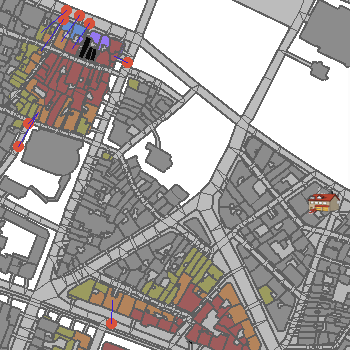
\includegraphics[width=.6\textwidth]{rcrs-detail}
    \caption[Detail of an example problem in the RCRS]{%
    Detail of an example RCRS problem on the Paris map. The red dots are fire brigades and
    the blue lines are their water jets. The colour of a building indicates its status:
    grey means no damage; yellow to red means on fire; blue to purple means that the fire
    has been extinguished, and black means that the building is burnt. The darker the
    colour, the greater the damage. On the centre-right is a fire station, to which the
    fire brigades return to refill. White regions indicate irrelevant areas, such as
    rivers or non-flammable properties.}
    \label{fig:rcrs}
\end{figure}

The RCRS is based on scenarios \cite{rcrsmanual}. A \emph{scenario} is a class of
problems, whose main parameter is the number of agents. In RMASBench there are $5$,
respectively with $15$, $21$, $27$, $33$ and $40$ fire brigades. Other settings are:
\begin{itemize}
    \item Agents are homogeneous, that is, they all have the same speed and water tank
        size;
    \item There are $3$ ignition points, and each scenario is replicated $30$ times. At
        each execution, a pseudo-random number generator influences the way the fires
        spread from ignition points to nearby buildings;
    \item To get a non-trivial number of fires, agents are added $25$ seconds after
        the start;
    \item Each simulation runs for a maximum of $5$ minutes, ending earlier if all fires
        have been extinguished;
    \item For each coalition $C$ and task $v$, we have that $u(C, v) = |C|$, which is a
        special case of superadditive characteristic function \cite[Section
        $2.1.2.2$]{chalkiadakis2011};
    \item Deadlines and workloads are randomly generated by the RCRS.
\end{itemize}
For each scenario and algorithm, we plot the average and standard deviation of:
\begin{enumerate}
    \item Problem completion time (Section \ref{sec:tests});
    \item The number of buildings that burned at least once, denoted by $b_{once}$;
    \item \emph{Score}, or the percentage of damage suffered by the city, where $100\%$
        means completely burnt. This is the main RCRS metric, defined on the total area of
        the city buildings and scenario-based parameters;
    \item Average CPU time\footnote{Based on an Intel Xeon E5-2670 processor ($2.6$ GHz,
        $16$ threads).} per problem time unit.
\end{enumerate}
We do not consider message-related metrics because agents do not communicate in S-CTS
(Section \ref{sec:s-cts}).

\subsection{Results}\label{sec:roboresults}

\begin{figure}[t]
    \centering
    \begin{adjustbox}{width=\textwidth}
        \begin{tikzpicture}
    \begin{groupplot}[%
            group style={group size=2 by 2, vertical sep=1.75cm, horizontal sep=1.75cm},
            grid=both,
            grid style={line width=.1pt, draw=gray!10},
            major grid style={line width=.2pt,draw=gray!50},
            minor tick num=5,
            ymin=0,
            xtick={15,21,27,33,40},
            legend style={/tikz/every even column/.append style={column sep=1em}, legend
            columns=-1,at={(0.35,2.55)}, anchor=north east},
            cycle list name=exotic3]

        \nextgroupplot[ymin=50,xlabel=Number of agents,ylabel=Problem completion time,
        title=(a)]

        % S-CTS
        \addplot+[error bars/.cd, y dir=both, y explicit,%
        error bar style = {thick}] coordinates {%
            (15, 167.97) +- (18.4, 18.4)
            (21, 162.14) +- (19.11, 19.11)
            (27, 130.94) +- (15.06, 15.06)
            (33, 97.94)  +- (10.38, 10.38)
            (40, 82.34)  +- (5.47, 5.47)
        };

        % DSA
        \addplot+[error bars/.cd, y dir=both, y explicit,%
        error bar style = {thick}] coordinates {%
            (15, 191.44) +- (19.7, 19.7)
            (21, 111.47) +- (13.98, 13.98)
            (27, 73.8)   +- (2.9, 2.9)
            (33, 65)     +- (1.39, 1.39)
            (40, 58.27)  +- (1.24, 1.24)
        };

        % BMS
        \addplot+[error bars/.cd, y dir=both, y explicit,%
        error bar style = {thick}] coordinates {%
            (15, 155.5) +- (19.04, 19.04)
            (21, 75.54) +- (3.95, 3.95)
            (27, 67.24) +- (1.35, 1.35)
            (33, 61.64) +- (0.64, 0.64)
            (40, 60.44) +- (1.09, 1.09)
        };

        \nextgroupplot[xlabel=Number of agents,ylabel=$b_{once}$, title=(b)]

        % S-CTS
        \addplot+[error bars/.cd, y dir=both, y explicit,%
        error bar style = {thick}] coordinates {%
            (15, 468.67) +- (105.57, 105.57)
            (21, 417.57) +- (96.05, 96.05)
            (27, 152.57) +- (48.29, 48.29)
            (33, 58.6) +- (18.42, 18.42)
            (40, 37.9) +- (5.34, 5.34)
        };

        % DSA
        \addplot+[error bars/.cd, y dir=both, y explicit,%
        error bar style = {thick}] coordinates {%
            (15, 587.1) +- (104.18, 104.18)
            (21, 186.54) +- (70.6, 70.6)
            (27, 32.87) +- (1.93, 1.93)
            (33, 29.64) +- (1.3, 1.3)
            (40, 26.54) +- (1.11, 1.11)
        };

        % BMS
        \addplot+[error bars/.cd, y dir=both, y explicit,%
        error bar style = {thick}] coordinates {%
            (15, 395.07) +- (98.67, 98.67)
            (21, 31.64) +- (2.77, 2.77)
            (27, 26.9) +- (0.83, 0.83)
            (33, 26) +- (0.8, 0.8)
            (40, 25.44) +- (0.84, 0.84)
        };

        \nextgroupplot[xlabel=Number of agents,ylabel=Score (\%), title=(b)]

        % S-CTS
        \addplot+[error bars/.cd, y dir=both, y explicit,%
        error bar style = {thick}] coordinates {%
            (15, 8.5108) +- (1.94, 1.94)
            (21, 9.86725) +- (2.27, 2.27)
            (27, 3.99635) +- (1.49, 1.49)
            (33, 1.43590) +- (0.31, 0.31)
            (40, 0.98847) +- (0.002, 0.002)
        };

        % DSA
        \addplot+[error bars/.cd, y dir=both, y explicit,%
        error bar style = {thick}] coordinates {%
            (15, 12.68) +- (2.375, 2.375)
            (21, 5.09) +- (1.93, 1.93)
            (27, 0.99) +- (0.0009, 0.0009)
            (33, 0.99175) +- (0.0004, 0.0004)
            (40, 0.99264) +- (0.0004, 0.0004)
        };

        % BMS
        \addplot+[error bars/.cd, y dir=both, y explicit,%
        error bar style = {thick}] coordinates {%
            (15, 6.63) +- (1.58, 1.58)
            (21, 0.99) +- (0.001, 0.001)
            (27, 0.99278) +- (0.0002, 0.0002)
            (33, 0.99325) +- (0.0001, 0.0001)
            (40, 0.99342) +- (0.0001, 0.0001)
        };

        \nextgroupplot[xlabel=Number of agents,ylabel=Average CPU time (ms), title=(d)]

        % S-CTS
        \addplot+[error bars/.cd, y dir=both, y explicit,%
        error bar style = {thick}] coordinates {%
            (15, 9.9) +- (1.76, 1.76)
            (21, 16.84) +- (3.44, 3.44)
            (27, 9.97) +- (2.465, 2.465)
            (33, 6.8) +- (0.68, 0.68)
            (40, 11.37) +- (0.57, 0.57)
        };

        % DSA
        \addplot+[error bars/.cd, y dir=both, y explicit,%
        error bar style = {thick}] coordinates {%
            (15, 24.54) +- (3.37, 3.37)
            (21, 19.97) +- (4.14, 4.14)
            (27, 17.57) +- (0.43, 0.43)
            (33, 23.1) +- (0.53, 0.53)
            (40, 44.34) +- (1.34, 1.34)
        };

        % BMS
        \addplot+[error bars/.cd, y dir=both, y explicit,%
        error bar style = {thick}] coordinates {%
            (15, 255.1) +- (44.11, 44.11)
            (21, 129.57) +- (4.87, 4.87)
            (27, 164.77) +- (3.4, 3.4)
            (33, 187.54) +- (7.14, 7.14)
            (40, 263.47) +- (6.63, 6.63)
        };

    \legend{\textsc{s-cts}, \textsc{dsa}, \textsc{binaryms}}
    \end{groupplot}
\end{tikzpicture}

    \end{adjustbox}
    \caption[Performance of S-CTS in RMASBench]{%
        Performance of S-CTS in RMASBench using DSA and Binary Max-Sum as baselines. In
        each figure, the X-axis defines the number of agents in the scenario, while each
        point is the $avg \pm std/2$, where $avg$ is the average over 30 simulations of
        the value indicated by the Y-axis, and $std$ is the standard deviation of $avg$.}
    \label{fig:c1test2}
\end{figure}

The more agents communicate with each other, the better they coordinate. In turn, this
leads to lower completion times and numbers of burned buildings. Because there is no
exchange of messages in S-CTS and BinaryMS has the highest communication overhead, they
are respectively the least and the most performing in Figures \ref{fig:c1test2}a and
\ref{fig:c1test2}b.
Nevertheless, this does not result in a drastic drop in performance. In Figure
\ref{fig:c1test2}c, in the worst-case scenario (i.e., $21$ agents), on average S-CTS
scores about $10\%$ (resp. $5\%$) less than BinaryMS (resp. DSA). This is not trivial,
given that S-CTS is a simplification and that the scenarios used are fine-tuned to
maximise the performance of BinaryMS and DSA.

Regarding the average CPU time (Figure \ref{fig:c1test2}d), S-CTS is up to two orders of
magnitude (resp. 1) faster than BinaryMS (resp. DSA). This is because BinaryMS has a
pre-processing phase that requires exponential time, while DSA, despite having a time
complexity similar to that of S-CTS (Table \ref{t:dcop_chars}), has a message-passing
phase as well.

In Figures \ref{fig:c1test2}a, \ref{fig:c1test2}b and \ref{fig:c1test2}c, the trends
converge to $0$ because the more agents there are, the less relevant the algorithm being
used becomes. In other words, the greater the number of available agents, the higher the
quality of solutions. We can deduce that the degree of agent communication is directly
proportional to the score and inversely proportional to the CPU time. However, as we have
seen, the difference in performance between communication and no communication is not
necessarily significant.

\section{Summary}

We presented CFLA2, a version of CFLA with a more detailed Phase $2$ and an improved Phase
$3$. Since we show that the time complexity of CFLA2 is quadratic in the number of tasks
and exponential in the number of agents, and that the look-ahead technique cannot be
used in dynamic environments, we also presented CTS, the first anytime and efficient
CFSTP algorithm with convergence guarantee. We demonstrated the superiority of CTS in
settings that largely favour the look-ahead technique, and showed that a simplified but
parallel variant is enough to compete with high-performance baselines in the RCRS,
at a fraction of their time complexity.
The next chapter extends CTS to large-scale dynamic and distributed environments, which
fall within our research objectives (Section \ref{sec:objectives}).

\chapter{Large-scale, Dynamic and Distributed CFSTP}\label{chap:contrib2}

After identifying the principal shortcomings in the CFSTP literature in Section
\ref{sec:cfstp-gaps}, this chapter proposes a minimal mathematical formulation in Section
\ref{sec:cfstp-bip}, a distributed version of CTS in Section \ref{sec:dcts}, and the first
large-scale, dynamic and distributed CFSTP test framework in Section \ref{sec:dcts-tests}.

\section{Major Gaps in the CFSTP Literature}\label{sec:cfstp-gaps}

There are $3$ main issues in the CFSTP literature. First, its original mathematical
programming formulation (Section \ref{sec:mip}) is based on $4$ sets of binary variables,
$1$ set of integer variables and $23$ types of constraints, $9$ of which use the Big-M
method. So many variables and constraints make implementation difficult, while the Big-M
method introduces a large penalty term that, if not chosen carefully, leads to serious
rounding errors and ill conditioning \cite[Section $5.4.2$]{griva2009}.

Second, there is no algorithm that is simultaneously scalable, distributed, and able to
solve the CFSTP in dynamic environments (Section \ref{sec:pstat}). To solve this issue, we
want to extend the CTS algorithm (Section \ref{sec:cts}), since it is anytime, has a
polynomial time complexity, and can be used in dynamic environments. Its only limitation
in relation to our objectives is to be centralised. In real-world domains such as disaster
response, this leads to problems such as single points of failure, unsustainable
computational loads, and poor performance in case of rapid changes of situation (Section
\ref{sec:pstat}).
To date, only \cite{ramchurn2010fms} have proposed a dynamic and distributed solution to
the CFSTP. They reduced it to a DynDCOP (Section \ref{sec:lit-dyndcop}) and solved it with
FMS, a variant of Max-Sum specialised for task allocation (Page \pageref{sec:lit-fms}).
However, unlike CTS, FMS is not guaranteed to converge, it is not anytime, and its
runtime is exponential in the number of agents. \cite{pujol2015} proposed BinaryMS
(Section \ref{sec:robotests}), another Max-Sum variant which, compared to FMS, lowers the
runtime to polynomial and achieves the same solution quality. Nonetheless, even BinaryMS
is not guaranteed to converge and not anytime. In addition, it requires a preprocessing
step with exponential runtime to transform the problem constraints into binary form,
which makes it not suitable for dynamic environments.

Lastly, no realistic CFSTP test framework has been proposed so far, although this
shortcoming was already identified in the original article \cite[Section
$8$]{ramchurn2010cfstp}. There are very few such frameworks even for the DynDCOP, to which
the CFSTP can be reduced, as mentioned above. Indeed, although the DCOP and DynDCOP models
can capture numerous real-world problems, researchers usually perform their empirical
evaluations on synthetic problems or classical combinatorial problems, such as graph
colouring and resource allocation \cite{fioretto2018survey}. To the best of our knowledge,
to date only the following (Dyn)DCOP works have conducted tests based on real-world data.
\cite{maheswaran2004b} considered resource-constrained multiple-event scheduling problems
occurring in office environments. \cite{junges2008} evaluated the performance of complete
DCOP algorithms in traffic light synchronisation problems. \cite{kim2011} developed
heuristics for applying Max-Sum to problems based on the real-time sensor system NetRad.
\cite{nelke2020,tkach2021} studied law enforcement problems inspired by police logs.
However, none of these test frameworks is large-scale\footnote{It is worth mentioning
\cite{leite2019a}, which is, to the best of our knowledge, the only study to date that
evaluates incomplete DCOP algorithms in large-scale problems, although not using
real-world data.}.
% shneider2020 also use real-world data, although their problem is a simpler MRTA

In the following sections, we address the above issues by proposing:
\begin{itemize}
    \item A novel mathematical programming formulation of the CFSTP, based only on binary
        variables and $5$ types of constraints, which do not use the Big-M method;
    \item A distributed version of the CTS algorithm that preserves its properties, namely
        being anytime, scalable and guaranteed to converge;
    \item The first large-scale, dynamic and distributed CFSTP test framework, based on
        real-world data published by the London Fire Brigade
        \cite{lfb-incident,lfb-mobilisation}.
\end{itemize}

\section{A Minimal Mathematical Program of the CFSTP}\label{sec:cfstp-bip}

We formulate the CFSTP as a \emph{Binary Integer Program} (BIP) \cite{wolsey2020}. Based
on the definitions of Sections \ref{sec:defs} $-$ \ref{sec:cv}, we detail our decision
variables, constraints and objective function.

\subsection{Decision variables}\label{sec:decvar}

Similar to Section \ref{sec:original-dv}, we use the following \emph{indicator} or binary
variables:
\begin{gather}
    \forall v \in V,\, \forall t \leq \gamma_v,\, \forall C \subseteq A,\;
    \mxc \in \left\{ 0, 1 \right\}\label{eq:bip0}\\
    \forall v \in V,\; y_v \in \left\{ 0, 1 \right\}\label{eq:bip0b}
\end{gather}
where: $\mxc = 1$ if coalition $C$ works on task $v$ at time $t$, and $0$ otherwise; $y_v
= 1$ if task $v$ is completed, and $0$ otherwise. Specifying indicator variables for
individual agents is not necessary, since they can be inferred from Equation
\ref{eq:bip0}.

\subsection{Constraints}\label{sec:bip-constraints}

There are $3$ types of constraints: structural, temporal and spatial.

\paragraph{Structural Constraints}

At each time, at most one coalition can work on each task:
\begin{equation}\label{eq:bip1}
    \forall v \in V,\, \forall t \leq
    \gamma_v,\; \sum_{C \subseteq A} \mxc \leq 1
\end{equation}
Equations \ref{eq:bip0} and \ref{eq:bip1} ensure that $\nexists \mxc : C \not\subseteq A$,
and that the maximum coalition size is $|A|$.

\paragraph{Temporal Constraints}

Tasks can be completed only by their deadlines, and no agent can work on a task after its
completion:
\begin{gather}
    \forall v \in V,\; y_v \leq 1\label{eq:bip2a}\\
    \forall v \in V,\;
    \left\lceil \sum_{t \leq \gamma_v}\, \sum_{C \subseteq A} u(C, v) \cdot \mxc
    \right\rceil = \left\lceil w_v \cdot y_v \right\rceil\label{eq:bip2b}
\end{gather}

\paragraph{Spatial Constraints}

An agent cannot work on a task before reaching its location. This identifies two cases:
when an agent reaches a task from its initial location, and when an agent moves from one
task location to another. The first case imposes that, for each task $v$, time $t \leq
\gamma_v$ and coalition $C$, the variable $\mxc$ can be positive only if all agents in $C$
can reach location $l_v$ at a time $t' < t$:
\begin{equation}\label{eq:bip3}
    \forall v \in V,\, \forall C \subseteq A,\;
    \text{if } \hat{\rho} = \max_{a \in C} \rho(a, l_a^0, l_v) \leq \gamma_v
    \text{ then }
    \sum_{t \leq \hat{\rho}}\, \mxc = 0
\end{equation}
where $\hat{\rho}$ is the maximum time at which an agent $a \in C$ reaches $l_v$, from its
initial location at time $t = 0$. Conditional constraints are usually formulated using
auxiliary variables or the Big-M method \cite{wolsey2020}.
However, such approaches further enlarge the mathematical program or can cause numerical
issues (Section \ref{sec:cfstp-gaps}). Consequently, in the preprocessing step necessary
to create our BIP, we can implement Equation \ref{eq:bip3} simply by excluding the
variables that must be equal to $0$. That is, if $\hat{\rho} \leq \gamma_v$, we only
declare the following variables: $\{ \mxc \}_{t \in [\hat{\rho} + 1, \gamma_v]}$.
The second case requires that if an agent cannot work on two tasks consecutively, then it
can work on at most one:
\begin{equation}\label{eq:bip4}
    \begin{gathered}
    \forall v_1, v_2 \in V,\,
    \forall C_1, C_2 \subseteq A \text{ such that } C_1 \cap C_2 \neq \emptyset,\\
    \forall t_1 \leq \gamma_{v_1},\, \forall t_2 \leq \gamma_{v_2} \text{ such that }
    t_1 + \max_{a \in C_1 \cap C_2} \rho(a, l_{v_1}, l_{v_2}) \geq t_2,\\
    x_{v_1,\, t_1, C_1} + x_{v_2,\, t_2, C_2} \leq 1
    \end{gathered}
\end{equation}
Hence, coalition $C_2$ can work on task $v_2$ only if all agents in $C_1 \cap C_2$ can
reach location $l_{v_2}$ by deadline $\gamma_{v_2}$. Equation \ref{eq:bip4} also implies
that an agent cannot work on multiple tasks at the same time.

There are no synchronisation constraints \cite{nunes2017taxonomy}. Thus, when a task $v$
is allocated to a coalition $C$, each agent $a \in C$ starts working on $v$ as soon as it
reaches its location, without waiting for the remaining agents. This means that $v$ is
completed by a temporal sequence of subcoalitions of $C$: $\exists S \subseteq P(C)$ such
that $\forall C' \in S$, $\exists t \leq \gamma_v$, $x_{v,\, t,\, C'} = 1$, where $P(C)$
is the power set of $C$.

\subsection{Objective Function}\label{sec:bip-of}

Let $\bm{x}$ be a \emph{solution}, that is, a value assignment to all variables, which
defines the route and schedule of each agent. The objective is to find a solution that
maximises the number of completed tasks:
\begin{equation}\label{eq:bip}
    \arg \max_{\bm{x}} \sum_{v \in V}\, y_v
    \text{ subject to Equations \ref{eq:bip0} $-$ \ref{eq:bip4}}
\end{equation}

Both creating all decision variables (Section \ref{sec:decvar}) and finding an optimal
solution exhaustively (Equation \ref{eq:bip}) may require to list all possible
coalition allocations for each possible permutation of $V$, with a worst-case time
complexity of:
\begin{equation}\label{eq:comp}
    O \left( |V|! \cdot 2^{|A|} \cdot \tmax \right)
\end{equation}
which is the same as the CFSTP formulation of Section \ref{sec:of}.

\begin{theorem}\label{teo:eq}
    Equation \ref{eq:bip} is equivalent to the original MIP of the CFSTP (Section
    \ref{sec:mip}).
\end{theorem}
\begin{proof}
    Since we use the original objective function (Equation \ref{eq:cfstpof}), below we
    show how our constraints imply the original ones (Equations \ref{eq:mip0} $-$
    \ref{eq:mip22}).

    Completing tasks by their deadlines and allowing agents to work only on uncompleted
    tasks implies that the total work done for each task $v$ is equal to $w_v$ if $v$ is
    completed, and $0$ otherwise. Hence, Equations \ref{eq:bip2a}, \ref{eq:bip2b}
    $\Rightarrow$ Equations \ref{eq:mip0}, \ref{eq:mip1}.

    Equation \ref{eq:bip1} is equivalent to Equation \ref{eq:mip2}.

    If at most one coalition can work on each task at each time, and an agent cannot
    work on a task before reaching its location, then each agent can work on at most one
    task at each time. Consequently, Equations \ref{eq:bip1}, \ref{eq:bip3} $\Rightarrow$
    Equation \ref{eq:mip6}.

    Equation \ref{eq:mip3} is not necessary because $t \leq \gamma_v$ for each $\mxc$
    (Equation \ref{eq:bip0}).

    If agent $a$ cannot work on task $v$ before reaching its location $l_v$, then it can
    do so after finishing work on a previous task, or after reaching $l_v$ from its
    initial location $l_0^a$. Furthermore, since the objective is to maximise the number
    of completed tasks, if $v$ is allocated to $a$, then $a$ changes the status of its
    service (from \emph{free} to \emph{working} and vice versa) exactly twice, and the
    decision variables related to $a$ and $v$ are equal to $1$ only when $a$ works on $v$,
    and $0$ otherwise. Thus, Equations \ref{eq:bip3} $-$ \ref{eq:bip} $\Rightarrow$
    Equations \ref{eq:mip4}, \ref{eq:mip5}, \ref{eq:mip7} $-$ \ref{eq:mip9}.

    If agent $a$ cannot work on two tasks consecutively, then it can work on at most one.
    Therefore, $a$ cannot leave and reach the same task location, it can only reach a new
    task location from exactly one location, and it can only leave a location to reach
    exactly one task location. That is, Equation \ref{eq:bip4} $\Rightarrow$ Equations
    \ref{eq:mip10} $-$ \ref{eq:mip12}.

    Since task $v$ can only be completed by deadline $\gamma_v$, agent $a$ can work on $v$
    only if it can reach its location $l_v$ by $\gamma_v$, and the objective is to
    maximise the number of completed tasks, then: the coalition $C$ of which $a$ is a
    member reaches $v$ only to complete it; $C$ works for at least $1$ unit of time on $v$
    (assuming that $w_v \geq 1$, $\forall v \in V$), and each $a \in C$ reaches $l_v$ from
    another task location or from its initial location $l_0^a$. Thus, Equations
    \ref{eq:bip2b} $-$ \ref{eq:bip4}, \ref{eq:bip} $\Rightarrow$ Equations \ref{eq:mip15} $-$
    \ref{eq:mip20}.

    Equation \ref{eq:bip1} is equivalent to Equation \ref{eq:mip21}.

    Since the original MIP assumes that the allocation process starts at $t = 1$ (Section
    \ref{sec:original-dv}), Equation \ref{eq:bip3} $\Rightarrow$ Equation \ref{eq:mip22}. If
    we remove this assumption, then Equation \ref{eq:mip22} is not necessary.
\end{proof}
Having significantly fewer constraints than the original MIP, our BIP can be used more
effectively by exact algorithms based on branch-and-cut or branch-and-price \cite[Section
$3.1.1$]{top2019}. A trivial way to solve the CFSTP would be to implement Equation
\ref{eq:bip} with solvers such as CPLEX or GLPK. Although this would guarantee anytime and
optimal solutions, it would also take exponential time to both create and solve our BIP
(Equation \ref{eq:comp}). This limits this practice to offline contexts and very small
problems. For example, using CPLEX $20.1$ with commodity hardware, and the test setup of
\cite{ramchurn2010cfstp}, we can solve problems where $|A| \cdot |V| \leq 20$ in hours.
With bigger problems, CPLEX depletes all memory ($8$ GB) and crashes.

Another major issue with centralised generation of optimal solutions is that, in real-time
domains such as disaster response, it can be computationally not feasible or economically
undesirable, especially when the problem changes frequently (Section \ref{sec:pstat}). For
these reasons, the next section presents a scalable, dynamic and distributed algorithm to
solve the CFSTP.

\section{A Scalable, Dynamic and Distributed CFSTP Algorithm}\label{sec:dcts}

We propose a novel reduction of the CFSTP to a DynDCOP, then we show how CTS can solve the
problem in this formulation. We use the DynDCOP formalism because it has proven largely
capable of modelling disaster response problems (Section \ref{chap2:choice}).

\subsection{Reduction of the CFSTP to a DynDCOP}\label{sec:reduction}

Using Definition \ref{def:dyndcop}, we formalise a DynDCOP as a sequence $\mathcal{D} =
\left\{ \mathcal{D}_t \right\}_{t \leq \tmax}$, where each $\mathcal{D}_t = (A^t, X^t,
D^t, F^t)$ is a DCOP such that $A^t \subseteq A$, and:
\begin{itemize}
    \item $X^t = \{\chi_1^t, \dots, \chi_k^t\}$ is a set of $k = |A^t| \leq n$ variables,
        where $\chi_i^t$ indicates the task performed by agent $a_i^t \in A^t$;
    \item $D^t = \{D_1^t, \dots, D_k^t\}$ is a set of $k$ variable domains, such that
        $\chi_i^t \in D_i^t$. A set $d = \{d_1, \dots, d_k\}$, where $d_i \in D_i^t$, is
        called an \emph{assignment}. Each $d_i \in d$ is called the $i$-th \emph{variable
        assignment} and is the value assigned to variable $\chi_i^t$;
    \item $F^t = \{f_1^t, \dots, f_h^t\}$ is a set of $h \leq m$ functions, where $f_i^t$
        represents the constraints on task $v_i^t$. In particular, each $f_i^t : D_{i_1}^t
        \times \cdots \times D_{i_{h_i}}^t \to \mathbb{R}_{\geq 0}$ assigns a non-negative
        real cost to each possible assignment to the variables $X_{h_i}^t \subseteq X^t$,
        where $h_i \leq h$ is the arity of $f_i^t$.
\end{itemize}
The objective of $\mathcal{D}$ is to find an assignment that minimises all costs:
\begin{equation}\label{eq:dcop}
    \forall t \leq \tmax,\, \arg \min_{d \in D^t}
    \sum_{f_i^t \in F^t} f_i^t(d_{i_1}, \dots, d_{i_{h_i}})
\end{equation}
It is typically assumed that if $\chi_i^t$ is in the scope of $f_j^t$, then agent $a_i^t$
knows $f_j^t$ \cite[Section $4.2$]{fioretto2018survey}. To reduce the CFSTP to a DynDCOP,
we specify $A^t$, $D^t$ and $F^t$ as follows. At time $t$, let $A^t$ be the set of free
agents (Section \ref{sec:cfla1}), and let $V^t_{allocable}$ be the set of tasks that have
not yet been completed. The domain of each variable $\chi_i^t$ is:
\begin{equation}\label{eq:dyndcop-d}
    D_i^t = \left\{ v \in V^t_{allocable} \text{ such that } t + \rho(a_i^t,
    l_{a_i^t}, l_v) \leq \gamma_v \right\} \cup \left\{ \varnothing \right\}
\end{equation}
where $\varnothing$ means that no task is allocated to agent $a_i^t$. Hence, $A^t$
satisfies the structural constraints, while $D_i^t$ contains all tasks that at time $t$
can be allocated to $a_i^t$ satisfying the spatial constraints (Section
\ref{sec:bip-constraints}). Let $\bm{x}_i \subseteq \bm{x}$ be a \emph{singleton
solution}, that is, a solution to task $v_i$ (Section \ref{sec:bip-of}). At time $t$, let
$\bm{x}_i^t \subseteq \bm{x}_i$ be a singleton solution corresponding to
$f_i^t(d_{i_1}, \dots, d_{i_{h_i}})$, defined as follows. Each $x_{v_i, \, t,\, C} \in
\bm{x}_i^t$ is such that $C$ is a subset of the agents that control the variables in
the scope of $f_i^t$, while $x_{v_i,\, t,\, C} = 1$ if $d_{i_{h_i}} = v_i$, for each
$h_i$-th agent in $C$, and $0$ otherwise. To satisfy the temporal constraints (Section
\ref{sec:bip-constraints}), each $i$-th function is defined as follows:
\begin{equation}\label{eq:costs}
    f_i^t(d_{i_1}, \dots, d_{i_{h_i}}) =
    \min_{\bm{x}_i^t,\, t' \leq \gamma_{v_i}}\, \left\lceil \sum_{s \leq t',\,
    x_{v_i,\, s,\, C} \in \bm{x}_i^t} u(C, v) \right\rceil = \left\lceil w_v \right\rceil
\end{equation}
with the convention that $f_i^t(d_{i_1}, \dots, d_{i_{h_i}}) = +\infty$ if $v_i$ cannot be
completed by deadline $\gamma_{v_i}$. Hence, the solution space of $\mathcal{D}$ satisfies
all CFSTP constraints, while minimising all costs implies minimising the time required to
complete each task (Equations \ref{eq:dcop} and \ref{eq:costs}), which implies maximising
the number of completed tasks, as required by the objective function of the CFSTP
(Equation \ref{eq:bip}).

\subsection{Distributed CTS}

Before introducing our distributed version of CTS (Section \ref{sec:cts}), we present the
data structure and the communication protocol on which it is based.

\begin{figure}[t]
    \centering
    \begin{adjustbox}{width=.45\textwidth}
        \begin{tikzpicture}
    \begin{scope}[square/.style={regular polygon,regular polygon sides=4}]
        \node (v1) at (-3, 0) [square,draw] {$f_1$};
        \node (v2) at (-1.5 , -1.5) [square,draw] {$f_2$};
        \node (v3) at (0 , 0) [square,draw] {$f_3$};
        \node (v4) at (1.5 , -1.5) [square,draw] {$f_4$};
        \node (a1) at (-1.5, 0) [circle,draw] {$\chi_1$};
        \node (a2) at (0 , -1.5) [circle,draw] {$\chi_2$};
    \end{scope}
    \begin{scope}
        \draw (a1) -- (v1);
        \draw (a1) -- (v2);
        \draw (a1) -- (v3);
        \draw (a2) -- (v2);
        \draw (a2) -- (v3);
        \draw (a2) -- (v4);
    \end{scope}
\end{tikzpicture}

    \end{adjustbox}
    \caption[An example factor graph]{The factor graph of a DCOP with $2$ agents and $4$
        tasks. In our formulation, a DCOP represents the state of a CFSTP at a certain
        time, in which circles are variables of free agents, squares are cost functions of
        uncompleted tasks, and each edge connects an agent to a task it can reach by its
        deadline.}
    \label{fig:fgex}
\end{figure}

To represent DCOPs, we use factor graphs (Definition \ref{def:fg}). As an example, Figure
\ref{fig:fgex} shows the factor graph of the function $F(X) = f_1(\chi_1) + f_2(\chi_1,
\chi_2) + f_3(\chi_1, \chi_2) + f_4(\chi_2)$. In a factor graph $G$, a solution is found
by allowing nodes to exchange messages. Hence, to execute CTS on $G$, we have to define
how nodes communicate and operate. Below, we present a communication protocol and
algorithms for both variable and factor nodes. Based on the well-established formalism of
\cite{yokoo1992}, the nodes communicate in the following way:
\begin{itemize}
    \item Node $i$ can message node $j$ only if $i$ knows the address of $j$\footnote{For
        instance, the IP address of $j$, if the nodes are connected to the same network.}.
        In our context, if $\chi_i^t$ is in the scope of $f_j^t$, then $\chi_i^t$ knows
        the address of $f_j^t$, and vice versa;
    \item Each node $i$ has a message queue $Q_i$, to which messages are delivered with a
        finite delay;
    \item Node $i$ can use the function \textsc{receive}() to dequeue a message from
        $Q_i$, and the function \textsc{send}($j$, \texttt{illoc\_force}, \texttt{[args]})
        to send a message to $j$. Node $j$ will receive a message in the format
        \texttt{(sender, illoc\_force, [args])}, where \texttt{sender} is the identifier
        of node $i$, \texttt{illoc\_force} is its illocutionary force, and \texttt{[args]}
        is an optional list of arguments. An \emph{illocutionary force} is either an
        information or a command \cite{vieira2007}.
\end{itemize}
We assume that the node of each function is controlled by an agent in its
scope\label{fgas}. This agent can be chosen randomly or according to some criterion.
Moreover, we assume that each agent can independently retrieve the system time (i.e., the
current value of $t$) in constant time.

Algorithm \ref{algo:d1} presents the operation of variable node $\chi_i^t$. If there is
an uncompleted task $v_j^t$ that can be allocated to free agent $a_i^t$ (lines $1 - 3$),
then variable node $\chi_i^t$ communicates to factor node $f_j^t$ the ability of $a_i^t$
to work on $v_j^t$, also specifying the time at which it can reach and start working on it
(lines $4 - 6$). After that, it waits until it gets a reply from $f_j^t$ or a
predetermined time interval expires (lines $7 - 9$). If it receives the approval of
$f_j^t$, then $v_j^t$ is allocated to $a_i^t$ (lines $10 - 11$). At line $2$, $v_j^t$ is
chosen such that it is the closest to $a_i^t$ and $\gamma_{v_j^t}$ is the earliest
deadline. Phase $1$ is completed after that each $\chi_i^t$ executes line $6$.

\begin{algorithm}[t]
    \DontPrintSemicolon
    $\chi_i^t \gets \varnothing$ \Comment*[h]{\small the agent is initially \emph{free}}\;
    $d_j \gets$ get task allocable to agent $a_i^t$ at time $t$ \Comment*[h]{\small
    Algorithm \ref{algo:getTask}}\;
    \If{$d_j \neq \varnothing$}{
        $s_i \gets$ time at which agent $a_i^t$ can start working on task $d_j$\;
        $f_j^t \gets$ factor node of $d_j$\;
        %create edge to $f_j^t$\;
        \textsc{send}($f_j^t$, \textsf{assignable}, $s_i$)\;
        \textsf{msg} $\gets$ \textsc{nil}\;
        \While{\normalfont\textsf{msg} not received from $f_j^t$ or not time out}{
            \textsf{msg} $\gets$ \textsc{receive}()\;
        }
        \If{\normalfont\textsf{msg} $= (f_j^t, \text{\textsf{allocate}})$}{
            $\chi_i^t \gets d_j$\;
        }
    }
    \caption{CTS node of variable $\chi_i^t$\label{algo:d1}}
\end{algorithm}

Algorithm \ref{algo:d2} presents the operation of factor node $f_j^t$. The loop at lines
$1 - 2$ is a synchronisation step that allows $f_j^t$ to know which agents in its
neighbourhood can work on $v_j^t$. Lines $3 - 6$ enacts Phase $2$, while lines $7 - 9$
update workload $w_{v_j}$.
Hence, our factor graphs are synchronous networks, in which the factor nodes are the
synchronisers \cite{lynch1996}.

\begin{algorithm}[t]
    \DontPrintSemicolon
    \While{\normalfont not all neighbours sent an \textsf{assignable} message or not time out}{
        \textsf{msg} $\gets$ \textsc{receive}()\;
    }
    $\Pi^t_{v_j} \gets$ list of all assignable agents sorted by arrival time to $v_j$\;
    %\Comment*[h]{\small same as line $19$ of Algorithm \ref{algo:cts}}\;
    $C^* \gets$ minimum coalition in $\Pi^t_{v_j}$ that can complete $v_j$ by $\gamma_{v_j}$
    \Comment*[h]{\small Equation \ref{eq:costs}}\;
    \For{$a_i^t \in C^*$}{
        \textsc{send}($\chi_i^t$, \textsf{allocate})\;
    }
    $C^t_{v_j} \gets$ all agents working on $v_j$ at time $t$\;
    \If{$C^t_{v_j} \neq \emptyset$}{
        $w_{v_j} \gets w_{v_j} - u(C^t_{v_j}, v_j)$\;
    }
    \caption{CTS node of factor $f_j^t$\label{algo:d2}}
\end{algorithm}

We call \emph{Distributed CTS} (D-CTS) the union of Algorithms \ref{algo:d1} and
\ref{algo:d2}. Each message has size $O(1)$, since it always contains a node
address, a message flag and an integer. At time $t$, each variable node $\chi_i^t$ sends
at most $1$ message (line $6$ in Algorithm \ref{algo:d1}), while each factor node $f_j^t$
sends $O(|A|)$ messages (lines $5 - 6$ in Algorithm \ref{algo:d2}). Assuming that all
tasks can be completed, the total number of messages sent is:
\begin{equation}\label{eq:dcts-co}
    O(|A| + |V| \cdot |A|) = O(|V| \cdot |A|)
\end{equation}
The runtime of Algorithm \ref{algo:d1} is $O(|V|)$, because line $2$ selects a task in the
neighbourhood of an agent. The runtime of Algorithm \ref{algo:d2} is $O(|A| \log |A|)$,
due to the sorting at line $3$ \cite{cormen2009}.
Since both algorithms are executed up to $\tmax$ times, the overall time complexity of
D-CTS is the same as CTS (Equations \ref{eq:comp1} and \ref{eq:comp2}).
The advantages of D-CTS are:
\begin{enumerate}
    \item
        It is anytime, since it decomposes a CFSTP into a set of subproblems (Section
        \ref{sec:cts}). This property is not trivial to guarantee in distributed systems
        \cite{zivan2014}, and is missing in main DCOP algorithms, such as ADOPT, DPOP,
        OptAPO and Max-Sum (Table \ref{t:dcop_chars});
    \item
        It is self-stabilising (Definition \ref{def:self-stabilising}), being guaranteed
        to converge (Theorem \ref{teo:convergence}), and given that each agent can only
        work on a new task after completing the one to which it is currently assigned
        (Algorithm \ref{algo:d1});
    \item
        The phase-based design has $2$ performance benefits. First, the algorithm is not
        affected by the structure of factor graphs. For instance, in a cyclic graph like
        the one in Figure \ref{fig:fgex}, where the same $a > 1$ tasks can be allocated to
        the same $b > 1$ agents, inference-based DCOP algorithms (e.g., Max-Sum variants)
        in general are not guaranteed to converge, unless they are augmented with specific
        techniques (e.g., damping or ADVP). Second, the algorithm is robust to
        \emph{disruptions}, that is, the addition or removal of factor graph nodes
        \cite[Section $6.2$]{ramchurn2010fms}. Disruptions are typical of dynamic
        environments (Section \ref{sec:pstat}). For instance, in disaster response, tasks
        are removed if some victims have perished, and are added if new fires are
        discovered. Likewise, new agents can be added to reflect the availability of
        additional workforce, while existing ones are removed when they deplete their
        resources, or are unable to continue due to sustained damages. Unlike D-CTS, the
        majority of DCOP algorithms (e.g., Max-Sum and DPOP) cannot handle disruptions,
        unless they are properly augmented (e.g., FMS and S-DPOP);
    \item
        Unlike most DCOP algorithms (e.g., ADOPT and DPOP), the communication overhead
        (i.e., the number of messages exchanged) is at most linear (Equation
        \ref{eq:dcts-co}), and each agent does not need to maintain an information graph
        of all other agents;
    \item
        Finally, performance does not depend on any tuning parameters, as is the case with
        other DCOP algorithms (e.g., DSA, AED and DPSA).
\end{enumerate}
Since each factor node is controlled by an agent (Page \pageref{fgas}), D-CTS is not fully
distributed, but \emph{partially centralised}. However, this is a typical assumption in
DCOP algorithms that use factor graphs or pseudo-trees, as it allows to explicitly handle
$k$-ary constraints \cite[Section $4.2$]{fioretto2018survey}. This is also the case for
main algorithms such as AFB, ADOPT, DPOP and Max-Sum (Section \ref{sec:dcop0}).
Partial centralisation improves local coordination and thus overall performance, but
reduces privacy \cite[Section $4.3.1$]{fioretto2018survey}.
In cooperative coordination, and particularly in disaster response, this is generally not
an issue.

Algorithms \ref{algo:d1} and \ref{algo:d2} resemble a \emph{single-item auction}
\cite{dias2006}, where, for each time $t$ and task $v_j$: the \emph{bidders} are the
agents in $A^t$ that can reach $v_j$ by $\gamma_{v_j}$; the \emph{bid} of an agent is the
time at which it can start working on $v_j$; the \emph{auctioneer} is the agent
controlling factor node $f^t_j$, which closes the auction by sending \textsf{allocate}
messages to selected agents.
However, there are two differences from a classic auction. First, $v_j$ can be
allocated to more than one agent at once.
Second, agents cannot be overburdened with evaluation problems, since each bidder is
interested in at most one task, and therefore each auctioneer receives as few bids as
possible. In other words, the communication overhead is minimised.
This advantage is due to our reduction of the CFSTP to a DynDCOP (Section
\ref{sec:reduction}), in which the search space contains only feasible solutions.

\section{Empirical Evaluation in Dynamic Environments}\label{sec:dcts-tests}

We created a dataset\footnote{\url{https://doi.org/10.5281/zenodo.4728012}} with $347588$
tasks using open records published by the \emph{London Fire Brigade} (LFB) over a period
of $11$ years. Then, we wrote a test framework in
Java\footnote{\url{https://doi.org/10.5281/zenodo.4764646}} and compared D-CTS with
DSA-SDP, a state-of-the-art incomplete, synchronous and search-based DCOP algorithm
(Page \pageref{sec:dsa}).

We adapted DSA-SDP to solve our DynDCOP formulation (Section \ref{sec:reduction}), which
finds a CFSTP solution by solving multiple DCOPs. Hence, being a DCOP algorithm, its
performance is not penalised in our test framework. We chose it as our baseline because,
similarly to D-CTS, it has a polynomial coordination overhead and is scalable (Table
\ref{t:dcop_chars}). We kept the parameters of \cite{zivan2014} and ran
$|V^t_{allocable}|$ iterations at each time $t$, since we found that, in our test
framework, running more iterations can only marginally improve the solution quality, while
requiring a significant increase in communication overhead and time complexity. Below, we
detail our setup and discuss the results.

\subsection{Setup}\label{sec:setup}

Let $\mathcal{N}$ and $\mathcal{U}$ denote the normal and uniform distribution,
respectively. A test configuration consists of the following parameters:
\begin{itemize}
    \item Since there are currently $150$ identical London fire engines in operation, $|A|
        = 150$ for each problem. All agents have the same speed;
        % It is reasonable to assume a fixed speed, because if an algorithm is better than
        % others with homogeneous agent speeds, then it is better with heterogeneous agent
        % speeds as well.
    \item $|V| = |A| \cdot k$, where $k \in \{ 1, \dots, 20 \}$. Thus, problems have up to
        $3000$ tasks;
    \item The demand of each task $v$ is defined by a record dated between $1$ January
        $2009$ and $31$ December $2020$. More precisely, $\gamma_v$ is the attendance time
        (in seconds) of the firefighters, and since the median attendance time in the
        whole dataset is about $5$ minutes, we set $w_v \sim \mathcal{U}(10, 300)$ to
        simulate wide-ranging workloads;
    \item For each task-to-agent ratio $|V|/|A|$, the nodes of a problem are chosen in
        chronological order. That is, the first problem always starts with record $1$, and
        if a problem stops at record $q$, then the following one will use records $q + 1$
        to $q + 1 + |V|$;
    \item The locations are latitude-longitude points, and the travel time $\rho(a, l_1,
        l_2)$ is given by the great-circle distance in kilometers between locations $l_1$
        and $l_2$, divided by the (fixed) speed of agent $a$;
    \item In addition to task locations, $L$ contains the locations of the $103$ currently
        active London fire stations. In each problem, each agent starts at a fire station
        defined by the record of a task.
\end{itemize}
Regardless of its individual features, each agent may perform differently in different
coalitions, due to the interaction with other agents. To generate coalition values, we
start by taking from \cite[Section $4$]{rahwan2012} the following well-known CSG
distributions:
\begin{enumerate}
    \item \emph{Normally Distributed Coalition Structures} (NDCS): $u(C, v) \sim
        \mathcal{N}(|C|, \sqrt[4]{|C|})$;
    \item \emph{Agent-based}: each agent $a$ has a value $p_a \sim \mathcal{U}(0,
        10)$ representing its individual performance and a value $p_a^C \sim
        \mathcal{U}(0, 2 \cdot p_a)$ representing its performance in coalition
        $C$. The value of a coalition is the sum of the values of its members:
        $u(C, v) = \sum_{a \in C} p_a^C$.
\end{enumerate}
Then, we decrease each $\mu_v = u(C, v)$ by values $r$ and $q$, both sampled from
$\mathcal{U}(\mu_v / 10, \mu_v / 4)$ with probability $\gamma_v/(\tmax + 1)$ and $|C|/(|A|
+ 1)$, respectively. The perturbation $r$ simulates real-time domains where the later
$\gamma_v$ is, the lower the benefit of performing $v$ \cite{stankovic2013edf}. The
perturbation $q$ simulates situations where the more agents there are, the greater the
likelihood of congestion and thus of reduced performance, as it can happen in large-scale
robot swarms \cite{guerrero2017}. We call the resulting distributions UC\_NDCS and
UC\_Agent-based, where UC means \emph{Urgent and Congested}. NDCS assigns lower values to
solutions containing fewer coalitions \cite{rahwan2009}, while Agent-based does the
opposite by definition. Both distributions are neither superadditive nor subadditive
\cite{rahwan2015survey}. Hence, it is not possible to define a priori an optimal coalition
for each task.
We ensured consistency between the results of the algorithms by computing and storing
coalition values in hash maps. More precisely, the maps were lazy-initialised and shared
among all problems.

During the solution of each problem, we gradually removed agents to simulate
\emph{degradation} scenarios. The removal rate was calculated with a Poisson cumulative
distribution function $Pois_{CDF}(\bm{a}, \lambda)$, where $\bm{a}$ contains all
firefighter arrival times in the dataset, and the rate $\lambda$ is the average number of
incidents per hour and per day. For each test configuration and algorithm, we solved
$100$ problems and measured the median and $95\%$ confidence interval of: number of
messages sent; \emph{network load}, or the total size of messages sent; number of
\emph{Non-Concurrent Constraint Checks} (NCCCs) \cite{meisels2007}; percentage of tasks
completed, and CPU time\footnote{Based on an Intel Xeon E5-2670 processor ($2.6$ GHz, $16$
threads).}.
% We do not measure problem completion times, because that makes sense only in static
% environments.

\subsection{Results}\label{sec:rres}

\begin{figure}[t]
    \centering
    \begin{adjustbox}{width=\textwidth}
        \begin{tikzpicture}
    \begin{groupplot}[%
        group style={group size=2 by 1, horizontal sep=2cm},
        grid=both,
        grid style={line width=.1pt, draw=gray!10},
        major grid style={line width=.2pt,draw=gray!50},
        xtick={1,4,8,12,16,20},
        every axis plot/.append style={thick},
        legend pos=north east]

        \large

        % Completed tasks

        \nextgroupplot[xlabel=$|V| / |A|$,ylabel=Completed tasks ($\%$),
        title=(a) UC\_NDCS, ymin=0, ymax=100, legend entries={\textsc{d-cts},
        \textsc{dsa-sdp}}]

        \addlegendimage{blue, line width=1.1}
        \addlegendimage{red,dashed, line width=1.1}

        %% DSA-SDP
        \addplot [dashed, red, line width=1.1] coordinates {%
            (1, 50)
            (2, 30)
            (3, 22)
            (4, 18)
            (5, 14)
            (6, 11)
            (7, 10)
            (8, 9)
            (9, 8)
            (10, 7)
            (11, 7)
            (12, 6)
            (13, 6)
            (14, 6)
            (15, 5)
            (16, 5)
            (17, 4)
            (18, 4)
            (19, 4)
            (20, 4)
        };

        \addplot [name path=u1, draw=none] plot coordinates {%
            (1, 54)
            (2, 32)
            (3, 24)
            (4, 19)
            (5, 15)
            (6, 12)
            (7, 11)
            (8, 10)
            (9, 9)
            (10, 8)
            (11, 7)
            (12, 7)
            (13, 6)
            (14, 6)
            (15, 5)
            (16, 5)
            (17, 5)
            (18, 4)
            (19, 4)
            (20, 4)
        };

        \addplot [name path=l1, draw=none] plot coordinates {%
            (1, 46)
            (2, 29)
            (3, 21)
            (4, 16)
            (5, 13)
            (6, 11)
            (7, 10)
            (8, 9)
            (9, 8)
            (10, 7)
            (11, 6)
            (12, 6)
            (13, 6)
            (14, 5)
            (15, 5)
            (16, 4)
            (17, 4)
            (18, 4)
            (19, 3)
            (20, 3)
        };

        \addplot+ [fill=red!25,postaction={pattern color = red!40, pattern=north
        west lines}] fill between[of=u1 and l1];

        %% D-CTS
        \addplot [blue, line width=1.1] coordinates {%
            (1, 99)
            (2, 51)
            (3, 34)
            (4, 27)
            (5, 23)
            (6, 19)
            (7, 16)
            (8, 15)
            (9, 13)
            (10, 12)
            (11, 11)
            (12, 11)
            (13, 10)
            (14, 9)
            (15, 8)
            (16, 8)
            (17, 7)
            (18, 7)
            (19, 6)
            (20, 6)
        };

        \addplot [name path=u2, draw=none] plot coordinates {%
            (1, 100)
            (2, 52)
            (3, 36)
            (4, 28)
            (5, 24)
            (6, 20)
            (7, 17)
            (8, 16)
            (9, 14)
            (10, 13)
            (11, 12)
            (12, 11)
            (13, 10)
            (14, 10)
            (15, 9)
            (16, 8)
            (17, 8)
            (18, 7)
            (19, 7)
            (20, 6)
        };

        \addplot [name path=l2, draw=none] plot coordinates {%
            (1, 98)
            (2, 50)
            (3, 34)
            (4, 26)
            (5, 21)
            (6, 18)
            (7, 16)
            (8, 15)
            (9, 13)
            (10, 12)
            (11, 11)
            (12, 10)
            (13, 9)
            (14, 9)
            (15, 8)
            (16, 7)
            (17, 7)
            (18, 6)
            (19, 6)
            (20, 5)
        };

        \addplot+ [fill=blue!25,opacity=0.6] fill between[of=u2 and l2];

        \nextgroupplot[xlabel=$|V| / |A|$,ylabel=Completed tasks ($\%$),
        title=(b) UC\_Agent-based, ymin=0, ymax=100,legend
        entries={\textsc{d-cts}, \textsc{dsa-sdp}}]

        \addlegendimage{blue,line width=1.1}
        \addlegendimage{red,dashed, line width=1.1}

        %% DSA-SDP
        \addplot [dashed, red, line width=1.1] coordinates {%
            (1, 58)
            (2, 35)
            (3, 26)
            (4, 21)
            (5, 17)
            (6, 15)
            (7, 13)
            (8, 11)
            (9, 10)
            (10, 9)
            (11, 9)
            (12, 8)
            (13, 7)
            (14, 7)
            (15, 7)
            (16, 6)
            (17, 6)
            (18, 5)
            (19, 5)
            (20, 4)
        };

        \addplot [name path=u1, draw=none] plot coordinates {%
            (1, 60)
            (2, 38)
            (3, 27)
            (4, 22)
            (5, 18)
            (6, 16)
            (7, 14)
            (8, 13)
            (9, 11)
            (10, 10)
            (11, 9)
            (12, 9)
            (13, 8)
            (14, 7)
            (15, 7)
            (16, 7)
            (17, 6)
            (18, 6)
            (19, 5)
            (20, 5)
        };

        \addplot [name path=l1, draw=none] plot coordinates {%
            (1, 57)
            (2, 34)
            (3, 25)
            (4, 20)
            (5, 16)
            (6, 14)
            (7, 12)
            (8, 11)
            (9, 10)
            (10, 9)
            (11, 8)
            (12, 7)
            (13, 7)
            (14, 6)
            (15, 6)
            (16, 6)
            (17, 5)
            (18, 4)
            (19, 4)
            (20, 4)
        };

        \addplot+ [fill=red!25,postaction={pattern color = red!40, pattern=north
        west lines}] fill between[of=u1 and l1];

        %% D-CTS
        \addplot [blue,line width=1.1] coordinates {%
            (1, 98)
            (2, 49)
            (3, 36)
            (4, 28)
            (5, 23)
            (6, 20)
            (7, 17)
            (8, 16)
            (9, 14)
            (10, 13)
            (11, 11)
            (12, 11)
            (13, 10)
            (14, 9)
            (15, 9)
            (16, 8)
            (17, 8)
            (18, 7)
            (19, 7)
            (20, 6)
        };

        \addplot [name path=u2, draw=none] plot coordinates {%
            (1, 98)
            (2, 52)
            (3, 37)
            (4, 29)
            (5, 25)
            (6, 21)
            (7, 18)
            (8, 16)
            (9, 14)
            (10, 13)
            (11, 12)
            (12, 11)
            (13, 10)
            (14, 9)
            (15, 9)
            (16, 8)
            (17, 8)
            (18, 7)
            (19, 7)
            (20, 7)
        };

        \addplot [name path=l2, draw=none] plot coordinates {%
            (1, 96)
            (2, 49)
            (3, 35)
            (4, 27)
            (5, 22)
            (6, 19)
            (7, 16)
            (8, 15)
            (9, 14)
            (10, 12)
            (11, 11)
            (12, 10)
            (13, 9)
            (14, 9)
            (15, 8)
            (16, 8)
            (17, 7)
            (18, 7)
            (19, 6)
            (20, 6)
        };

        \addplot+ [fill=blue!25, opacity=0.6] fill between[of=u2 and l2];
    \end{groupplot}
\end{tikzpicture}

    \end{adjustbox}
    \caption[Comparison between D-CTS and DSA-SDP]{Comparison between D-CTS and DSA-SDP in
        our test framework. Each subfigure denotes a coalition value distribution, while
        each point is the median and $95\%$ confidence interval over $100$ problems of the
        percentage of tasks completed. The X-axis is the task-to-agent ratio.}
    \label{fig:dcts-t}
\end{figure}

% UC_AGENT_BASED 1.35 \pm [0.29, 0.03] -> 3.03% \pm [34.98, 1.2]
% UC_NDCS 1.6 \pm [0.26, 0.06] -> 4.76% \pm [41.24, 2.76]
% Overall 1.52 \pm [0.33, 0.21] -> 3.79% \pm [42.22, 1.96]
Figure \ref{fig:dcts-t} and \ref{fig:dcts-t2} show our results. D-CTS completes $3.79\%
\pm [42.22\%, 1.96\%]$ more tasks than DSA-SDP (Figure \ref{fig:dcts-t}). For both
algorithms, the performance drops rapidly as the task-to-agent ratio increases. This is
due to the Urgent component in the coalition value distributions: the higher the ratio,
the higher the median task completion time.
Conversely, the Congested component can reduce the percentage of tasks completed more in
problems with smaller task-to-agent ratios, where agents can form larger coalitions and
thus increase the likelihood of congestion.

The network load of DSA-SDP is $0.59 \pm [0.41, 0.02]$ times that of D-CTS (Figure
\ref{fig:dcts-t2}b). This is because a DSA-SDP message contains only a task address,
while a D-CTS message also contains a binary flag and an integer (Section
\ref{sec:dcts}). In Java, an address requires $8$ bytes, a flag requires $1$ byte, and
an integer requires $1 - 4$ bytes. Hence, while a DSA-SDP message always requires $8$
bytes, a D-CTS message requires $10 - 13$ bytes. This is line with the results obtained.
However, the situation would be reversed if we performed $1000$ DSA-SDP iterations as
suggested in \cite{zhang2005}, since $median(\{ |V^t_{allocable}| \}_{t \leq \tmax}) \ll
1000$ in our tests.

\begin{figure}[t]
    \centering
    \begin{adjustbox}{width=\textwidth}
        \begin{tikzpicture}
    \begin{groupplot}[%
        group style={group size=2 by 2, vertical sep=2.25cm, horizontal sep=2cm},
        grid=both,
        grid style={line width=.1pt, draw=gray!10},
        major grid style={line width=.2pt,draw=gray!50},
        every axis plot/.append style={very thick},
        %y tick label style={/pgf/number format/sci},
        xtick={1,4,8,12,16,20},
        legend style={draw=none,/tikz/every even column/.append %
        style={column sep=1em},legend columns=-1,at={(1.75,1.35)}}]

        \large

        % Messages sent

        \nextgroupplot[xlabel=$|V| / |A|$, ylabel=DSA-SDP / D-CTS,
        title={(a) Messages sent},legend entries={\textsc{uc\_ndcs},
        \textsc{uc\_agent-based}}]

        \addlegendimage{no markers,mycol1,line width=2.0,loosely dashed}
        \addlegendimage{no markers,mycol2,line width=2.0}

        %% UC_NDCS
        \addplot [dashed,mycol1,line width=1.1] coordinates {%
            (1, 54.41)
            (2, 52.58)
            (3, 48.99)
            (4, 46.32)
            (5, 46.16)
            (6, 44.68)
            (7, 44.58)
            (8, 42.29)
            (9, 41.96)
            (10, 41.59)
            (11, 40.88)
            (12, 39.96)
            (13, 39.65)
            (14, 40.27)
            (15, 40.70)
            (16, 39.45)
            (17, 40.30)
            (18, 39.78)
            (19, 41.77)
            (20, 43.01)
        };

        \addplot [name path=u2, draw=none] plot coordinates {%
            (1, 55.60)
            (2, 52.79)
            (3, 50.06)
            (4, 48.06)
            (5, 46.76)
            (6, 45.80)
            (7, 45.87)
            (8, 43.42)
            (9, 43.21)
            (10, 43.85)
            (11, 42.32)
            (12, 41.46)
            (13, 41.65)
            (14, 41.34)
            (15, 42.86)
            (16, 42.07)
            (17, 44.78)
            (18, 43.75)
            (19, 45.13)
            (20, 47.51)
        };

        \addplot [name path=l2, draw=none] plot coordinates {%
            (1, 53.49)
            (2, 50.99)
            (3, 47.49)
            (4, 45.23)
            (5, 44.50)
            (6, 43.15)
            (7, 42.51)
            (8, 40.51)
            (9, 39.36)
            (10, 39.41)
            (11, 39.31)
            (12, 38.03)
            (13, 38.09)
            (14, 37.73)
            (15, 38.29)
            (16, 37.47)
            (17, 37.66)
            (18, 37.19)
            (19, 37.82)
            (20, 38.35)
        };

        \addplot+ [fill=mycol1!25, opacity=0.6] fill between[of=u2 and l2];

        %% UC_Agent-based
        \addplot [mycol2, line width=1.1] coordinates {%
            (1, 57.56)
            (2, 55.13)
            (3, 51.38)
            (4, 49.13)
            (5, 46.14)
            (6, 44.74)
            (7, 44.30)
            (8, 42.85)
            (9, 42.01)
            (10, 41.54)
            (11, 41.60)
            (12, 41.68)
            (13, 41.41)
            (14, 40.77)
            (15, 39.88)
            (16, 39.94)
            (17, 40.03)
            (18, 40.92)
            (19, 40.67)
            (20, 41.26)
        };

        \addplot [name path=u1, draw=none] plot coordinates {%
            (1, 58.62)
            (2, 54.17)
            (3, 49.91)
            (4, 47.57)
            (5, 44.18)
            (6, 43.37)
            (7, 42.62)
            (8, 41.71)
            (9, 40.98)
            (10, 40.74)
            (11, 40.65)
            (12, 40.26)
            (13, 40.63)
            (14, 40.20)
            (15, 39.18)
            (16, 39.08)
            (17, 38.63)
            (18, 38.75)
            (19, 38.51)
            (20, 39.87)
        };

        \addplot [name path=l1, draw=none] plot coordinates {%
            (1, 55.80)
            (2, 55.50)
            (3, 52.39)
            (4, 49.86)
            (5, 47.59)
            (6, 45.37)
            (7, 45.98)
            (8, 43.23)
            (9, 42.87)
            (10, 42.85)
            (11, 42.54)
            (12, 42.62)
            (13, 43.37)
            (14, 41.45)
            (15, 41.71)
            (16, 41.64)
            (17, 41.30)
            (18, 41.73)
            (19, 43.94)
            (20, 45.34)
        };

        \addplot+ [fill=mycol2!25,opacity=0.6,postaction={pattern color = mycol2!40, pattern=north east lines}] fill between[of=u1 and l1];

        % Network load
        \nextgroupplot[xlabel=$|V| / |A|$, ylabel=DSA-SDP / D-CTS,
        title={(b) Network load}]

        %% UC_NDCS
        \addplot [dashed,mycol1,line width=1.1] coordinates {%
            (1, 0.88)
            (2, 0.79)
            (3, 0.74)
            (4, 0.69)
            (5, 0.66)
            (6, 0.64)
            (7, 0.64)
            (8, 0.60)
            (9, 0.59)
            (10, 0.58)
            (11, 0.58)
            (12, 0.56)
            (13, 0.56)
            (14, 0.53)
            (15, 0.57)
            (16, 0.55)
            (17, 0.56)
            (18, 0.56)
            (19, 0.57)
            (20, 0.60)
        };

        \addplot [name path=u2, draw=none] plot coordinates {%
            (1, 0.92)
            (2, 0.79)
            (3, 0.74)
            (4, 0.70)
            (5, 0.69)
            (6, 0.67)
            (7, 0.66)
            (8, 0.62)
            (9, 0.63)
            (10, 0.61)
            (11, 0.61)
            (12, 0.59)
            (13, 0.58)
            (14, 0.57)
            (15, 0.59)
            (16, 0.60)
            (17, 0.60)
            (18, 0.62)
            (19, 0.64)
            (20, 0.66)
        };

        \addplot [name path=l2, draw=none] plot coordinates {%
            (1, 0.88)
            (2, 0.78)
            (3, 0.71)
            (4, 0.67)
            (5, 0.63)
            (6, 0.62)
            (7, 0.61)
            (8, 0.58)
            (9, 0.56)
            (10, 0.55)
            (11, 0.54)
            (12, 0.54)
            (13, 0.53)
            (14, 0.52)
            (15, 0.54)
            (16, 0.52)
            (17, 0.52)
            (18, 0.51)
            (19, 0.52)
            (20, 0.53)
        };

        \addplot+ [fill=mycol1!25, opacity=0.6] fill between[of=u2 and l2];

        %% UC_Agent-based
        \addplot [mycol2,line width=1.1] coordinates {%
            (1, 0.99)
            (2, 0.85)
            (3, 0.76)
            (4, 0.72)
            (5, 0.67)
            (6, 0.63)
            (7, 0.64)
            (8, 0.60)
            (9, 0.59)
            (10, 0.58)
            (11, 0.59)
            (12, 0.57)
            (13, 0.58)
            (14, 0.56)
            (15, 0.55)
            (16, 0.55)
            (17, 0.54)
            (18, 0.55)
            (19, 0.55)
            (20, 0.57)
        };

        \addplot [name path=u1, draw=none] plot coordinates {%
            (1, 0.99)
            (2, 0.82)
            (3, 0.74)
            (4, 0.69)
            (5, 0.63)
            (6, 0.62)
            (7, 0.60)
            (8, 0.59)
            (9, 0.57)
            (10, 0.57)
            (11, 0.57)
            (12, 0.55)
            (13, 0.55)
            (14, 0.55)
            (15, 0.53)
            (16, 0.53)
            (17, 0.53)
            (18, 0.53)
            (19, 0.53)
            (20, 0.54)
        };

        \addplot [name path=l1, draw=none] plot coordinates {%
            (1, 0.99)
            (2, 0.86)
            (3, 0.78)
            (4, 0.73)
            (5, 0.69)
            (6, 0.65)
            (7, 0.66)
            (8, 0.61)
            (9, 0.61)
            (10, 0.60)
            (11, 0.61)
            (12, 0.59)
            (13, 0.60)
            (14, 0.58)
            (15, 0.57)
            (16, 0.57)
            (17, 0.58)
            (18, 0.58)
            (19, 0.59)
            (20, 0.62)
        };

        \addplot+ [fill=mycol2!25,opacity=0.6,postaction={pattern color = mycol2!40, pattern=north east lines}] fill between[of=u1 and l1];

        % NCCCs

        \nextgroupplot[xlabel=$|V| / |A|$, ylabel=DSA-SDP / D-CTS,
        title={(c) NCCCs}]

        %% UC_NDCS
        \addplot [dashed,mycol1,line width=1.1] coordinates {%
            (1, 99.97)
            (2, 91.34)
            (3, 83.46)
            (4, 79.80)
            (5, 79.59)
            (6, 74.60)
            (7, 70.52)
            (8, 67.96)
            (9, 66.43)
            (10, 63.96)
            (11, 69.10)
            (12, 70.82)
            (13, 64.34)
            (14, 56.91)
            (15, 62.32)
            (16, 55.12)
            (17, 60.25)
            (18, 56.48)
            (19, 60.88)
            (20, 64.98)
        };

        \addplot [name path=u2, draw=none] plot coordinates {%
            (1, 100.78)
            (2, 94.72)
            (3, 88.09)
            (4, 83.16)
            (5, 85.67)
            (6, 81.82)
            (7, 74.18)
            (8, 72.85)
            (9, 72.04)
            (10, 70.45)
            (11, 80.55)
            (12, 80.43)
            (13, 72.45)
            (14, 67.39)
            (15, 71.75)
            (16, 62.41)
            (17, 73.47)
            (18, 66.66)
            (19, 70.50)
            (20, 71.98)
        };

        \addplot [name path=l2, draw=none] plot coordinates {%
            (1, 98.96)
            (2, 85.65)
            (3, 81.40)
            (4, 77.82)
            (5, 68.54)
            (6, 68.24)
            (7, 63.78)
            (8, 59.46)
            (9, 58.70)
            (10, 59.60)
            (11, 65.20)
            (12, 62.14)
            (13, 55.43)
            (14, 44.99)
            (15, 55.28)
            (16, 47.78)
            (17, 55.58)
            (18, 55.09)
            (19, 57.73)
            (20, 59.34)
        };

        \addplot+ [fill=mycol1!25, opacity=0.6] fill between[of=u2 and l2];

        %% UC_Agent-based
        \addplot [mycol2,line width=1.1] coordinates {%
            (1, 106.27)
            (2, 104.65)
            (3, 93.27)
            (4, 89.44)
            (5, 84.36)
            (6, 85.06)
            (7, 82.49)
            (8, 81.25)
            (9, 77.98)
            (10, 80.19)
            (11, 77.19)
            (12, 72.95)
            (13, 67.72)
            (14, 72.61)
            (15, 69.04)
            (16, 69.13)
            (17, 72.69)
            (18, 71.09)
            (19, 70.29)
            (20, 63.54)
        };

        \addplot [name path=u1, draw=none] plot coordinates {%
            (1, 106.66)
            (2, 107.58)
            (3, 97.56)
            (4, 94.58)
            (5, 88.11)
            (6, 87.21)
            (7, 86.16)
            (8, 82.10)
            (9, 89.49)
            (10, 89.26)
            (11, 81.45)
            (12, 80.58)
            (13, 78.65)
            (14, 85.32)
            (15, 82.78)
            (16, 79.14)
            (17, 86.91)
            (18, 84.66)
            (19, 74.39)
            (20, 80.18)
        };

        \addplot [name path=l1, draw=none] plot coordinates {%
            (1, 105.03)
            (2, 101.43)
            (3, 91.25)
            (4, 85.03)
            (5, 81.25)
            (6, 80.50)
            (7, 75.37)
            (8, 75.06)
            (9, 67.18)
            (10, 73.13)
            (11, 67.03)
            (12, 64.18)
            (13, 64.06)
            (14, 67.36)
            (15, 61.67)
            (16, 64.66)
            (17, 68.79)
            (18, 63.25)
            (19, 63.53)
            (20, 58.40)
        };

        \addplot+ [fill=mycol2!25,opacity=0.6,postaction={pattern color = mycol2!40, pattern=north
        east lines}] fill between[of=u1 and l1];

        % CPU time

        \nextgroupplot[xlabel=$|V| / |A|$, ylabel=DSA-SDP / D-CTS,
        title={(d) CPU time}]

        %% UC_NDCS
        \addplot [dashed,mycol1,line width=1.1] coordinates {%
            (1, 8.50)
            (2, 9.28)
            (3, 9.49)
            (4, 9.25)
            (5, 10.96)
            (6, 11.55)
            (7, 10.68)
            (8, 11.00)
            (9, 11.53)
            (10, 12.47)
            (11, 13.32)
            (12, 12.66)
            (13, 14.65)
            (14, 14.42)
            (15, 15.53)
            (16, 16.17)
            (17, 16.28)
            (18, 18.25)
            (19, 20.93)
            (20, 21.40)
        };

        \addplot [name path=u2, draw=none] plot coordinates {%
            (1, 10.50)
            (2, 10.10)
            (3, 10.91)
            (4, 12.27)
            (5, 12.63)
            (6, 12.53)
            (7, 11.95)
            (8, 11.89)
            (9, 13.24)
            (10, 14.01)
            (11, 15.85)
            (12, 14.53)
            (13, 16.24)
            (14, 15.44)
            (15, 17.21)
            (16, 17.31)
            (17, 19.81)
            (18, 22.63)
            (19, 24.24)
            (20, 24.70)
        };

        \addplot [name path=l2, draw=none] plot coordinates {%
            (1, 7.43)
            (2, 6.70)
            (3, 7.47)
            (4, 7.34)
            (5, 8.96)
            (6, 9.61)
            (7, 9.12)
            (8, 9.00)
            (9, 9.97)
            (10, 11.02)
            (11, 11.88)
            (12, 11.44)
            (13, 12.26)
            (14, 13.00)
            (15, 13.31)
            (16, 12.96)
            (17, 14.58)
            (18, 15.18)
            (19, 16.81)
            (20, 17.02)
        };

        \addplot+ [fill=mycol1!25, opacity=0.6] fill between[of=u2 and l2];

        %% UC_Agent-based
        \addplot [mycol2,line width=1.1] coordinates {%
            (1, 8.49)
            (2, 10.52)
            (3, 11.96)
            (4, 12.38)
            (5, 11.22)
            (6, 11.73)
            (7, 11.56)
            (8, 12.24)
            (9, 13.15)
            (10, 14.31)
            (11, 14.44)
            (12, 14.95)
            (13, 15.96)
            (14, 16.23)
            (15, 16.19)
            (16, 17.92)
            (17, 18.63)
            (18, 19.48)
            (19, 20.96)
            (20, 21.74)
        };

        \addplot [name path=u1, draw=none] plot coordinates {%
            (1, 9.00)
            (2, 12.18)
            (3, 12.73)
            (4, 13.93)
            (5, 14.40)
            (6, 13.68)
            (7, 13.51)
            (8, 13.52)
            (9, 14.14)
            (10, 15.52)
            (11, 15.60)
            (12, 17.02)
            (13, 17.41)
            (14, 17.46)
            (15, 18.68)
            (16, 19.62)
            (17, 20.80)
            (18, 24.15)
            (19, 23.25)
            (20, 27.50)
        };

        \addplot [name path=l1, draw=none] plot coordinates {%
            (1, 7.31)
            (2, 9.38)
            (3, 9.74)
            (4, 9.76)
            (5, 9.86)
            (6, 10.52)
            (7, 10.59)
            (8, 11.01)
            (9, 11.35)
            (10, 12.45)
            (11, 12.25)
            (12, 13.58)
            (13, 13.70)
            (14, 14.51)
            (15, 14.61)
            (16, 15.72)
            (17, 16.49)
            (18, 17.40)
            (19, 18.05)
            (20, 18.34)
        };

        \addplot+ [fill=mycol2!25,opacity=0.6,postaction={pattern color = mycol2!40, pattern=north east lines}] fill between[of=u1 and l1];
    \end{groupplot}
\end{tikzpicture}

    \end{adjustbox}
    \caption[Ratio of DSA-SDP performance to D-CTS performance]{%
        Ratio of DSA-SDP performance to D-CTS performance. Each subfigure denotes a
        performance metric $m$, while each point is the median and $95\%$ confidence
        interval over $100$ problems of $m_a / m_b$, where $m_a$ (resp. $m_b$) is the
        value of DSA-SDP (resp. D-CTS) for $m$. The X-axis is the task-to-agent ratio.}
    \label{fig:dcts-t2}
\end{figure}

The remaining metrics put DSA-SDP at a distinct disadvantage (Figure \ref{fig:dcts-t2}a,
c, d). The overload compared to D-CTS is $41.72 \pm [12.45, 0.42]$ times more messages
sent, $72.78 \pm [34.79, 27.79]$ times more NCCCs, and $13.82 \pm [4.52, 3.71]$ times more
CPU time. This is explained as follows. While the number of messages sent is $O(|V| \cdot
|A|)$ in D-CTS (Section \ref{sec:dcts}), it is $O(|V| \cdot |A|^2)$ in DSA-SDP, since the
agents exchange their assignments\footnote{To align with Table \ref{t:dcop_chars}, we have
that $t = |V|$, and $n = l = |A|$.} \cite{zivan2014}. In D-CTS, analysing in sequence the
agents that can be assigned to each task (line $4$ in Algorithm \ref{algo:d2}) requires
$O(|V| \cdot |A|)$ NCCCs. DSA-SDP does a similar analysis, but for each message exchanged
between two agents, which requires $O(|V|^2 \cdot |A|^2)$ NCCCs. Finally, the time
complexity of DSA-SDP is $O(\tmax \cdot |V| \cdot |A|^2)$, where $O(|V| \cdot |A|)$ is
required by the message exchange phase at each time, and $O(|A|)$ is required by each
agent to calculate the assignment costs (Equation \ref{eq:costs}). Hence, DSA-SDP is
asymptotically slower than D-CTS (Equations \ref{eq:comp1} and \ref{eq:comp2}). Overall,
D-CTS took $525 \pm [281, 482]$ ms, while DSA-SDP took $6.97 \pm [5.84, 6.2]$ seconds. In
accordance with the above, the ratio of DSA-SDP performance to D-CTS performance tends to
increase with regard to CPU time, and to decrease with regard to the other metrics.

In a dynamic environment, desirable features of a distributed algorithm include being
robust to disruptions and minimising communication overhead (Section \ref{sec:dcts}).
The latter feature is particularly important in real-world domains such as disaster
response, where agent communication can be costly (i.e., not free-comm environments,
Section \ref{sec:mdp}) or there may be operational constraints, such as low bandwidth or
limited network topology (e.g., sparse robot swarms searching for shipwrecks on the
seabed, or monitoring forest fires \cite{tarapore2020}). In our tests, compared to the
state-of-the-art DSA-SDP, D-CTS achieves a slightly better solution quality (Figure
\ref{fig:dcts-t}), and is one order of magnitude more efficient in terms of communication
overhead and time complexity (Figure \ref{fig:dcts-t2}). This affirms its effectiveness as
a scalable and distributed CFSTP algorithm for dynamic environments.

\section{Summary}

We proposed a novel and minimal BIP of the CFSTP, and demonstrated its equivalence with
the original MIP formulation (Section \ref{sec:mip}). Based on a novel reduction of the
CFSTP to a DynDCOP, we also created D-CTS, a distributed version of CTS that preserves its
properties (anytime, convergent, scalable) and is self-stabilising. We defined a
large-scale CFSTP dataset, as well as a dynamic test framework, and empirically showed
that D-CTS has slightly better performance than the state-of-the-art DSA-SDP, while having
significantly lower communication overhead and time complexity. Having filled the main
gaps in the literature, in order to meet all our research objectives (Section
\ref{sec:objectives}), the next and final chapter will focus on the main limitations of
the CFSTP model itself.

\chapter{The Multi-Agent Routing and Scheduling through Coalition Formation
Problem}\label{chap:contrib3}

Although many problems similar to the CFSTP have been studied to date (Section
\ref{chap2:limitations}), no one can meet all our research objectives (Section
\ref{sec:objectives}). Against this background, in this final chapter we begin by
presenting in Section \ref{sec:marsc} the \emph{Multi-Agent Routing and Scheduling through
Coalition formation problem} (MARSC), a generalisation of the CFSTP and the TOPTW that can
be used in real-time domains. Then, we define in Section \ref{sec:ant} the first anytime,
exact and parallel MARSC algorithm. Since no exact algorithm has so far been proposed for
the CFSTP, it is consequently the first of its kind for this problem as well. Finally, in
Section \ref{sec:marsc-tests}, using extended versions of the test frameworks of Chapters
\ref{chap:contrib1} and \ref{chap:contrib2}, we evaluate our algorithm on synthetic
small-scale problems, and an approximate variant on large-scale realistic problems.

\section{Problem Formulation}\label{sec:marsc}

As in Section \ref{sec:cfstp-bip}, we use a BIP formulation. Since the MARSC generalises
the CFSTP (Theorem \ref{teo:cfstp-gen}),
we recall and extend the basic definitions and constraints of Sections \ref{sec:defs} $-$
\ref{sec:cv} and \ref{sec:cfstp-bip}.
Specifically, we add multiple possible locations per task, benefits, time windows,
precedences, and define a more general objective function.
We also show how to extend the work of Section \ref{sec:reduction} to reduce the MARSC to
a DynDCOP.

\subsection{Basic Definitions}\label{sec:marsc-defs}

Let $V = \{ v_1, \dots, v_m \}$ be a set of $m$ tasks and $A = \{ a_1, \dots, a_n \}$ be a
set of $n$ agents. Let $L$ be the finite set of all possible task and agent locations.
Time is denoted by $t \in \mathbb{N}$, starting at $t = 0$, and agents travel or perform
tasks with a base time unit of $1$. The time units needed by an agent to travel from one
location to another are given by the function $\rho : A \times L \times L \rightarrow
\mathbb{N}$. Having $A$ in the domain of $\rho$ allows to characterise different agent
features (e.g., speed or type). Let $l_a^t \in L$ be the location of agent $a$ at time
$t$, where $l_a^0$ is the initial location of $a$ and is known a priori.

\paragraph{Task Demand}

Each task $v$ has a \emph{demand} $D_v = (L_v, w_v, \phi_v, \alpha_v, \beta_v, \gamma_v)$,
where:
\begin{itemize}
    \item $L_v \subseteq L$ is the \emph{set of possible locations of} $v$;
    \item $w_v \in \mathbb{R}_{\geq 0}$ is the \emph{workload} of $v$, or the amount of
        work required to complete $v$;
    \item $\phi_v \in \mathbb{R}_{\geq 0}$ is the \emph{benefit} of $v$, or the weight
        associated with the completion of $v$;
    \item $\left[ \alpha_v, \beta_v, \gamma_v \right]$ is the \emph{time window} of $v$,
        such that $\alpha_v \in \mathbb{N}$ is the \emph{earliest time} of $v$, or the
        time starting from which agents can work on $v$, $\beta_v \in \mathbb{N}$ is the
        \emph{soft latest time} of $v$, or the time until which agents can work on $v$
        without incurring in a penalty, and $\gamma_v \in \mathbb{N}$ is the \emph{hard
        latest time} of $v$, or the time until which agents can work on $v$ incurring in a
        penalty. No agent can work on $v$ after $\gamma_v$.
\end{itemize}
We assume that $\alpha_v \leq \beta_v \leq \gamma_v$, $\forall v \in V$, and call $\tmax
=$ $\max_{v \in V} \gamma_v$ the \emph{maximum problem time}.

\paragraph{Task Order}\label{sec:ordering}

Let $Prec \subseteq V \times V$ be such that if $(v_1, v_2) \in Prec$ then $v_1$ must be
completed before $v_2$. Each $(v_1, v_2) \in Prec$ is called a \emph{precedence} and can
be graphically denoted with $v_1 \prec v_2$. As typically done in MRTA
\cite{nunes2017taxonomy}, we assume that $G = (V, Prec)$ is a finite, directed and acyclic
graph. Moreover, without loss of generality, we assume that $Prec$ does not contain
relations which can be inferred transitively, that is:
\begin{equation*}
    (v_1, v_2) \in Prec \land (v_2, v_3) \in Prec \Rightarrow (v_1, v_3) \not\in Prec
\end{equation*}

\paragraph{Coalition and Coalition Value}\label{sec:marsc-cv}

A subset of agents $C \subseteq A$ is called a \emph{coalition}. For each coalition, task
and location there is a \emph{coalition value}, given by the function $u : P(A) \times V
\times L \rightarrow \mathbb{R}_{\geq 0}$, where $P(A)$ is the power set of $A$. The
value of $u(C, v, l)$ is the amount of work that coalition $C$ does on task $v$ at
location $l \in L_v$ in one time unit. In other words, when $C$ performs $v$ in $l$,
$u(C, v, l)$ expresses how well the agents in $C$ work together, and the workload $w_v$
decreases by $u(C, v, l)$ at each time.

\subsection{Decision Variables}\label{sec:marsc-ca}

We use the following indicator variables:
\begin{gather}
    \forall v \in V,\, \forall l \in L_v,\, \forall t \in [\alpha_v,
    \gamma_v],\,
    \forall C \subseteq A,\;
    \mx \in \left\{ 0, 1 \right\}\label{eq:mbip0}\\
    \forall v \in V,\, \forall l \in L_v,\; y_{v, l} \in \left\{ 0, 1 \right\}\label{eq:mbip0b}
\end{gather}
where: $\mx = 1$ if task $v$ in location $l$ and at time $t$ is performed by coalition
$C$, and $0$ otherwise; $y_{v, l} = 1$ if task $v$ is completed in location $l$, and $0$
otherwise.

\subsection{Constraints}\label{sec:marsc-constraints}

There are $4$ types of constraints: structural, temporal, spatial and ordering.
%We formalise each below.

\paragraph{Structural Constraints}

Each task can be performed by at most one coalition at each time, and only within its time
window:
\begin{equation}\label{eq:mbip1}
    \forall v \in V,\, \forall l \in L_v,\, \forall t \in [\alpha_v, \gamma_v],\;
    \sum_{C \subseteq A} \mx \leq 1
\end{equation}

\paragraph{Temporal Constraints}

Each task can be performed in at most one location, and no agent can work on it after its
workload has been completed:
\begin{gather}
    \forall v \in V,\; \sum_{l \in L_v} y_{v, l} \leq 1\label{eq:mbip2a}\\
    \forall v \in V,\, \forall l \in L_v,\;
    \left\lceil \sum_{t \in [\alpha_v, \gamma_v]}\, \sum_{C \subseteq A} u(C, v, l)
    \cdot \mx \right\rceil
    = \left\lceil w_v \cdot y_{v, l} \right\rceil\label{eq:mbip2b}
\end{gather}

\paragraph{Spatial Constraints}

An agent cannot work on a task before reaching one of its possible locations. This
identifies two cases: when an agent reaches a task location from its initial location, and
when an agent moves from one task location to another. The first case imposes that, for
each task $v$, location $l \in L_v$ and coalition $C$, the decision variable $\mx$ can be
positive only if all agents in $C$ can reach $l$ at time $t' < t$:
\begin{equation}\label{eq:mbip3}
    \forall v \in V,\, \forall l \in L_v,\, \forall C \subseteq A,\,
    \text{if } \hat{\rho} = \max_{a \in C} \rho(a, l_a^0, l) \geq \alpha_v
    \text{ then }
    \sum_{t \in [\alpha_v, \hat{\rho}]}\, \mx = 0
\end{equation}
The value of $\hat{\rho}$ is the maximum time at which an agent $a \in C$ reaches $l$,
from its initial location at time $t = 0$. Conditional constraints are usually formulated
using auxiliary variables or the Big-M method. However, such approaches further enlarge
the mathematical program or easily cause numerical issues (Section \ref{sec:cfstp-gaps}).
Consequently, in the preprocessing step necessary to create our BIP, we can implement
Equation \ref{eq:mbip3} simply by excluding the variables that must be equal to $0$.
%That is, if $\hat{\rho} \leq \gamma_v$, we only declare the following variables: $\{ \mx
%\}_{t \in [\hat{\rho} + 1, \gamma_v]}$.
The second case requires that if an agent cannot perform two tasks consecutively, then it
can perform at most one:
\begin{equation}\label{eq:mbip4}
    \begin{gathered}
    \forall C_1, C_2 \subseteq A : C_1 \cap C_2 \neq \emptyset,\,
    \forall v_1, v_2 \in V,\, \forall l_1 \in L_{v_1},\, \forall l_2 \in L_{v_2},\\
    \forall t_1 \in [\alpha_1, \gamma_1],\, \forall t_2 \in [\alpha_2, \gamma_2] :
    t_1 + \max_{a \in C_1 \cap C_2} \rho(a, l_1, l_2) \geq t_2,\\
    x_{v_1,\, l_1,\, t_1, C_1} + x_{v_2,\, l_2,\, t_2, C_2} \leq 1
    \end{gathered}
\end{equation}
Hence, coalition $C_2$ can perform task $v_2$ only if all agents in $C_1 \cap C_2$ can
reach location $l_2$ by the hard latest time $\gamma_2$. Equation \ref{eq:mbip4} also
implies that two tasks cannot be performed by the same agent at the same time.
Consequently, coalitions that exist in different locations at the same time are disjoint.
There are no synchronisation constraints \cite{nunes2017taxonomy}. Thus, when a task $v$
in location $l$ is allocated to a coalition $C$, each agent $a \in C$ starts working on
$v$ as soon as it reaches $l$, without waiting for the remaining agents. That is, $v$ is
completed by a temporal sequence of subcoalitions of $C$: $\exists S \subseteq P(C)$ such
that $\forall C' \in S$, $\exists t \in [\alpha_v, \gamma_v]$, $x_{v,\, l,\, t,\, C'} =
1$, where $P(C)$ is the power set of $C$.

\paragraph{Ordering Constraints}

If $v_1 \prec v_2$ then $v_2$ can only be performed after $v_1$:
\begin{equation}\label{eq:mbip5}
    \forall v_1, v_2 \in V,\, \text{if } v_1 \prec v_2 \text{ then }
    \sum_{l_1 \in L_{v_1}} y_{v_1, l_1} \geq \sum_{l_2 \in L_{v_2}} y_{v_2, l_2}
\end{equation}

\subsection{Objective Function}\label{sec:ofmarsc}

Let $\bm{x}$ be a \emph{solution}, that is, a value assignment to all decision variables,
which defines the route and schedule of each agent. For each task $v$ and time $t$, let:
\begin{equation}\label{eq:penalty}
\psi_{v, t} =
\begin{cases}
    1, & \quad\text{if } t \leq \beta_v\\
    1 - \dfrac{t - \beta_v}{\gamma_v - \beta_v + 1}, & \text{ otherwise}
\end{cases}
\end{equation}
be the \emph{penalty} of performing $v$ at $t$, that is, a positive weight that decreases
linearly after $t$ passes $\beta_v$. Let:
\begin{equation}\label{eq:score}
    score(\bm{x}) =
    \sum_{v \in V}\, \sum_{l \in L_v}\, \sum_{t \in [\alpha_v, \gamma_v]}\,
    \sum_{C \subseteq A}\, \phi_v \cdot \psi_{v, t} \cdot \mx
\end{equation}
be the \emph{score} of $\bm{x}$.
The objective of the MARSC is to find a solution that has maximum score and satisfies all
constraints:
\begin{equation}\label{eq:mbip}
    \arg \max_{\bm{x}} score(\bm{x})
    \text{ subject to Equations \ref{eq:mbip0} $-$ \ref{eq:mbip5}}
\end{equation}
Hence, Equation \ref{eq:mbip} maximises the total benefit while minimising the total time
penalty (i.e., the number of tasks that are completed after their soft latest times).
This involves maximising task completion times and minimising coalition sizes.
Consequently, the number of tasks performed at any one time is the largest, and the most
beneficial tasks are prioritised. Ours is a combination of two objective functions
commonly used in MRTA problems \cite[Section $5$]{nunes2017taxonomy}.
Creating all decision variables (Equation \ref{eq:mbip0}) may require to list all
$\mathcal{L}$-tuples over $P(A)$, where $\mathcal{L} = |V| \cdot |L| \cdot
\tmax$. This implies a worst-case time and space complexity of:
\begin{equation}\label{eq:mccc}
    O\left( {\left(2^{|A|}\right)}^{\mathcal{L}} \right) =
    O\left( 2^{|A| \cdot |V| \cdot |L| \cdot \tmax} \right)
\end{equation}
In addition, searching for an optimal solution exhaustively (Equation \ref{eq:mbip}) may
require to list all possible coalition allocations for each possible permutation of $V$,
with a worst-case time complexity of:
\begin{equation}\label{eq:mcomp}
    O \left( |V|! \cdot |L| \cdot 2^{|A|} \cdot \tmax \right)
\end{equation}

\begin{theorem}\label{teo:cfstp-gen}
    The MARSC generalises the CFSTP.
\end{theorem}
\begin{proof}
We refer to the BIP formulation of the CFSTP given in Section \ref{sec:cfstp-bip}.

The CFSTP is a MARSC where tasks have exactly one location, benefits are homogeneous,
there are neither earliest nor soft latest times, and tasks can be completed in any order.
The structural, temporal and spatial constraints are identical. Given a MARSC solution
$\bm{x}$ and a task $v$, if $\mx = 1$, for some $l \in L_v$, $t \in [\alpha_v, \gamma_v]$
and $C \in P(A)$, then $y_{v, l} = 1$. Thus, in the presence of the above-mentioned
simplifications, Equation \ref{eq:mbip} maximises the number of completed tasks, as
required by the objective function of the CFSTP (Equation \ref{eq:bip}).
\end{proof}

\begin{theorem}\label{teo:toptw-gen}
    The MARSC generalises the TOPTW.
\end{theorem}
\begin{proof}
Based on \cite[Section $3.3$]{top2019}, we first describe the TOPTW using our terminology
(Section \ref{sec:marsc-defs}), then we show that it is a special case of the MARSC.

The TOPTW considers a finite set of tasks, each with a non-negative benefit. Each task has
exactly one location and no soft latest time: $|L_v| = 1 \,\land\, \beta_v = \gamma_v$,
$\forall v \in V$. When a task is completed within its time window, its benefit is added
to the total benefit. Between each pair of tasks there is a fixed travel time. There are
an initial task and a final task, both with a benefit of $0$, an earliest time of $0$ and
a soft latest time of $\tmax$. Each route must begin at the location of the initial task
and end at the location of the final task. The objective is to determine $n$ routes, one
for each agent, that maximise the total benefit.

The travel time between tasks $v_i$ and $v_j$ also includes the \emph{service time} at
$v_j$, that is, the time taken by any coalition to complete $v_j$ \cite[Section
$2.2$]{top2019}. Hence, we set $w_v = 1$, $\forall v \in V$, to ensure that each task is
completed in at most $1$ unit of time. Since travel times depend only on task locations,
we exclude $A$ from the domain of $\rho(\cdot)$. Coalitions are singleton, that is, each
$C$ is such that $|C| = 1$. The coalition value function $u(\cdot)$ always returns $1$.

Because each task has exactly one location and coalitions are singleton, we remove the
subscript $l$ from the decision variables and simply use $a$ instead of $C$ to indicate
the coalition that consists of agent $a$. Hence: $x_{v,\, t,\, a} = 1$ if agent $a$ works
on task $v$ at time $t$, and $0$ otherwise; $y_v = 1$ if task $v$ is completed, and $0$
otherwise. Let $v_{start}$ and $v_{end}$ denote the initial and final tasks, respectively.
The structural constraints (Equation \ref{eq:mbip1}) become:
\begin{equation}
    \forall v \in V \setminus \left\{ v_{start}, v_{end} \right\},\,
    \forall t \in [\alpha_v, \beta_v],\;
    \sum_{a \in A} x_{v,\, t,\, a} \leq 1\label{eq:tops}
\end{equation}
Since both coalition values and workloads are unitary, and each task does not have
multiple locations, Equation \ref{eq:tops} already ensures that a task is completed within
its time window by at most one agent. Hence, no temporal constraints (Equations
\ref{eq:mbip2a} and \ref{eq:mbip2b}) are required.

Let $l_{start}$ denote the location of $v_{start}$, and let $l_v$ denote the location of
any other task $v$. The initial location of each agent is $l_{start}$, and the spatial
constraints (Equations \ref{eq:mbip3} and \ref{eq:mbip4}) become:
\begin{equation}
    \forall v \in V,\, \forall a \in A,\,
    \text{if } \lambda = \rho(l_{start}, l_v) \geq \alpha_v \text{ then }
    \sum_{t \in [\alpha_v, \lambda]} x_{v,\, t,\, a} = 0
\end{equation}
\begin{equation}
\begin{gathered}
    \forall v_1, v_2 \in V,\, \forall a \in A,\,
    \forall t_1 \in [\alpha_1, \beta_1],\, \forall t_2 \in [\alpha_2, \beta_2]
    : t_1 + \rho(l_{v_1}, l_{v_2}) \geq t_2,\\
    x_{v_1,\, t_1,\, a} + x_{v_2,\, t_2,\, a} \leq 1
\end{gathered}
\end{equation}
To ensure that each agent schedule starts with $v_{start}$ and ends with $v_{end}$, we
define the set of precedences as follows:
\begin{equation*}
    Prec = \left\{ (v_{start}, v), (v, v_{end}) : v \in V \setminus \left\{ v_{start},
    v_{end} \right\} \right\}
\end{equation*}
The ordering constraints (Equation \ref{eq:mbip5}) become:
\begin{equation}
    \forall v_1, v_2 \in V,\, \text{if } v_1 \prec v_2 \text{ then }
    y_{v_1} \geq y_{v_2}\label{eq:topf}
\end{equation}
The absence of soft latest times means that there can be no time penalties: $\psi_{v,t} =
1$, $\forall v \in V$, $\forall t \leq \tmax$ (Equation \ref{eq:penalty}). Hence, the
objective function (Equation \ref{eq:mbip}) is simplified as follows:
\begin{equation}
    \begin{gathered}
    \arg \max_{\bm{x}} \sum_{v \in V \setminus \{v_{start}, v_{end}\}}\,
    \sum_{t \in [\alpha_v, \beta_v]}\,
    \sum_{a \in A} \phi_v \cdot x_{v,\, t,\, a}\\
    \text{subject to Equations \ref{eq:tops} $-$ \ref{eq:topf}}
    \end{gathered}
    \label{eq:topof}
\end{equation}
\end{proof}

Both the CFSTP and the TOPTW are NP-hard \cite{ramchurn2010cfstp,top2019}, thus the MARSC
is NP-hard as well.
%\clearpage

\subsection{Reduction of the MARSC to a DynDCOP}\label{sec:reduction2}

Given that the MARSC generalises the CFSTP (Theorem \ref{teo:cfstp-gen}), to reduce it to
a DynDCOP, there are two modifications to be made to the work of Section
\ref{sec:reduction}.

Let $V^t_{completed}$ denote the set of tasks that have been completed at time $t$. The
first modification is to include ordering constraints and the possibility of having
multiple possible locations per task by redefining Equation \ref{eq:dyndcop-d} as follows:
\begin{equation}
    \begin{gathered}
    D_i^t = \big\{
        v \in V^t_{allocable} \,|
        \left(\exists v_2 \in V : v_2 \prec v \Rightarrow v_2 \in V^t_{completed} \right)
        \;\land\\ \exists l \in L_v : t + \rho(a_i^t, l_{a_i^t}, l) \leq \gamma_v \big\}
        \cup \left\{ \varnothing \right\}
    \end{gathered}
\end{equation}
Recall that, in propositional logic, $A \Rightarrow B \equiv \neg A \lor B \equiv
\text{if } A \text{ then } B$.
The second change is to include time windows, benefits and penalties by redefining
Equation \ref{eq:costs} as follows:
\begin{equation}\label{eq:costs2}
    f_i^t(d_{i_1}, \dots, d_{i_{h_i}}) = \min_{\bm{x}_i^t}\, - score(\bm{x}_i^t)
\end{equation}
where each $x_{v_i,\, l,\, t,\, C} \in \bm{x}_i^t$ is such that $C$ is a subset of the
agents that control the variables in the scope of $f_i^t$, while $x_{v_i,\, l,\, t,\, C} =
1$ if $d_{i_{h_i}} = v_i$, for each $h_i$-th agent in $C$ and for some $l \in L_{v_i}$,
and $0$ otherwise.
Being an additive function (Equation \ref{eq:score}), the solution score fits naturally
with the characterisation of $f_i^t(\cdot)$. It is multiplied by $-1$ in Equation
\ref{eq:costs2} because we formulate the DynDCOP as a minimisation problem (Equation
\ref{eq:dcop}).

\section{An Anytime, Exact and Parallel MARSC Algorithm}\label{sec:ant}

A trivial way to solve the MARSC would be to implement Equation \ref{eq:mbip} with solvers
such as CPLEX or GLPK. Although this would guarantee anytime and optimal solutions, it
would also take exponential time and space to create the BIP (Equation \ref{eq:mccc}), in
addition to the time to solve it (Equation \ref{eq:mcomp}). This limits this practice to
offline contexts and very small problems. For example, using CPLEX $20.1$ with our HPC
cluster\footnote{\href{https://www.southampton.ac.uk/isolutions/staff/iridis.page}{The
Iridis $5$ Compute Cluster at the University of Southampton}.}, we can solve within hours
problems with superadditive coalition values, uniformly distributed workloads and time
windows, locations based on the taxicab metric, and $dim = |A|\cdot|V|\cdot|L| \leq 30$.
With greater $dim$ values, CPLEX depletes all memory ($187.5$ GB) and crashes. For this
reason, this section presents the \emph{Anytime, exact and parallel Node Traversal} (ANT)
algorithm, which provides the sharp lower bound on the time and space complexity required
to solve the MARSC optimally. We begin by explaining its procedures, then we analyse its
theoretical properties and computational complexity.
%\clearpage

\subsection{Procedures}\label{sec:procedures}

\begin{algorithm}[t]
    \DontPrintSemicolon
    \KwIn{task $v$, location $l \in L_v$, agents $A'$}
    $\Pi_v \gets$ array of all agents in $A'$ that, from their current \textsf{status},
    can reach $l$ by $\gamma_v$\;
    Sort $\Pi_v$ by arrival time to $l$\;
    $\varphi_v \gets 0$ \Comment{\small total workload done on $v$}
    \For{$i \gets 1$; $i \leq |\Pi_v|$; $i \gets i + 1$}{
        $C^\ast \gets$ first $i$ agents in $\Pi_v$\;
        $\lambda_i \gets$ arrival time to $l$ of the $i$-th agent in $\Pi_v$\;
        \eIf{$i + 1 \leq |\Pi_v|$}{
            $\lambda_{i+1} \gets$ arrival time to $l$ of the $(i+1)$-th agent in
            $\Pi_v$\;
        }(\Comment*[h]{\small the $i$-th agent is the last}){
            $\lambda_{i+1} \gets \gamma_v$ \Comment{\small last feasible working time}
        }
        $\varphi_v \gets \varphi_v + (\lambda_{i+1} - \lambda_i) \cdot u(C^\ast,
        v, l)$ \Comment{\small workload done at time $\lambda_{i+1}$}
        \If{$(\gamma_v - \lambda_{i+1}) \cdot u(C^\ast, v, l) \geq w_v -
            \varphi_v$}{
            \Return $\bm{x}_v$ \Comment{\small using $C^\ast$, $v$, and $l$}
        }
    }
    \Return \textsc{nil}\;
    \caption{\textsf{getSingletonSolution}\label{algo:getSingletonSolution}}
\end{algorithm}

\begin{algorithm}[t]
    \DontPrintSemicolon
    \KwIn{incumbent solution $\bm{x}$, task permutation $V^\alpha$, agents $A'$}
    $\bm{x}^\alpha \gets$ empty vector\;
    \For{$v \in V^\alpha$}{
        $\bm{x}_v^\alpha \gets$ \textsc{nil}\;
        \For{$l \in L_v$}{
            $\bm{x}_{v,l}^\alpha \gets$ \textsf{getSingletonSolution($v$, $l$, $A'$)}\;
            $\bm{x}_v^\alpha \gets \arg \max_{\bm{x}' \in \{\bm{x}_{v,l}^\alpha,
            \bm{x}_v^\alpha\}}
            score(\bm{x}')$\;
        }
        \If{$\bm{x}_v^\alpha \neq$ \normalfont{\textsc{nil}}}{
            $\forall a \in A'$, update $a$\textsf{.status} based on $\bm{x}_v^\alpha$\;
        }
    }

    \Return $\arg \max_{\bm{x}' \in \{\bm{x}^\alpha,
    \bm{x}\}} score(\bm{x'})$ \Comment{\small access to $\bm{x}$ is synchronised}
    \caption{\textsf{getSolutionForSchedule}\label{algo:getSolutionForSchedule}}
\end{algorithm}

Given a task $v$, a location $l \in L_v$ and a set of agents $A' \subseteq A$, Algorithm
\ref{algo:getSingletonSolution} defines a coalition $C^\ast \subseteq P(A')$ such that
$|C^\ast|$ is minimum and each agent $a \in C^\ast$ reaches $l$ not only by $\gamma_v$
(line $1$), but also in the shortest possible time (line $2$), which satisfies the spatial
constraints. The \textsf{status} of each agent (line $1$) is set by Algorithm
\ref{algo:getSolutionForSchedule}. When the condition at line $12$ holds, $C^\ast$
satisfies the temporal constraints. Line $13$ returns a singleton solution $\bm{x}_v
\subseteq \bm{x}$ (Section \ref{sec:reduction}). In particular, $\bm{x}_v$ defines the
temporal sequence of subcoalitions of $C^\ast$ that are formed as the agents reach $l$,
thus satisfying the structural constraints.
That is, for each $a \in C^\ast$, $\bm{x}_v$ defines the time interval $i$ during which
$a$ will work on $v$ at $l$, such that $i$ does not violate any constraints, and
$score(\bm{x}_v)$ is maximum; $a$ is considered part of $C^\ast$ from the moment
$\bm{x}_v$ is created until the end of $i$.

Let $\sigma(V)$ denote the set of all permutations of $V$. Algorithm
\ref{algo:getSolutionForSchedule} takes as input a task permutation $V^\alpha \subseteq
\sigma(V)$ and a set of agents $A' \subseteq A$. It defines a solution $\bm{x}^\alpha$ by
finding singleton solutions following the order of $V^\alpha$. For each $v \in V^\alpha$,
the loop at line $4$ finds a location $l \in L_v$ that maximises $score(\bm{x}_v^\alpha)$,
with the convention that $score(\text{\textsc{nil}}) = 0$.
Lines $7$ and $8$ ensure that $\bm{x}^\alpha$ satisfies the structural constraints by
saving, after finding each singleton solution and for each agent $a \in A'$, the last time
$a$ was working, and at which location (i.e., its \textsf{status}).
%This information is used by Algorithm \ref{algo:getSingletonSolution} to define $\Pi_v$.
At line $9$, $\bm{x}$ is maximised synchronously to allow execution in concurrent
environments.

\begin{algorithm}[t]
    \DontPrintSemicolon
    \KwIn{tasks $V$, demands $\{D_v\}_{v \in V}$, order $Prec$, agents $A$}
    $\bm{x} \gets$ empty vector\;
    Sort $V$ by earliest time, while satisfying the ordering constraints
    \Comment{\small initial schedule}
    $\bm{x} \gets$ \textsf{getSolutionForSchedule($\bm{x}$, $V$, $\text{clone}(A)$)}
    \Comment{\small initial incumbent solution}
    \For(\Comment*[h]{\small remaining schedules}){$V^\alpha \in \sigma(V)$}{
        \If{$V^\alpha$ \textnormal{satisfies the ordering constraints}}{
            $\bm{x} \gets$ \textsf{getSolutionForSchedule($\bm{x}$, $V^\alpha$,
            $\text{clone}(A)$)}\;
            \If{$\exists k \leq |V| : \nexists$ \textnormal{solutions for} $k$
                \textnormal{tasks in} $\bm{x}$}{
                \Break
            }
        }
    }
    \Return $\bm{x}$\;
    \caption{ANT\label{algo:ant}}
\end{algorithm}

Algorithm \ref{algo:ant} describes the overall procedure. Lines $2$ and $3$ initialise the
incumbent solution using the \emph{Earliest Deadline First} (EDF) technique, which is
typically used in real-time systems \cite{stankovic2013edf}. Lines $4 - 6$ launch a thread
with an instance of Algorithm \ref{algo:getSolutionForSchedule} for each \emph{schedule}
or permutation of $V$ that satisfies the ordering constraints. At lines $3$ and $6$, $A$
is cloned to avoid interferences between threads. The stopping criterion at line $7$ works
as follows. Let $k$ be the number of tasks performed in the solution found at line $6$,
let $S$ be the set of all schedules investigated so far, and let $\tilde{X}$ be the set of
all solutions found so far. If for each permutation of $k$ tasks $p$ there is a schedule
in $S$ that starts with $p$, and $\tilde{X}$ does not contain a solution involving $k$
tasks, then there can be no solution for $k' \geq k$ tasks. Since $S$ consequently also
contains schedules starting with each permutation of $k'' < k$ tasks, the search can
safely end.

The reason why it is sufficient that, for each $k$-permutation of tasks $p$, $S$ contains
a schedule $s$ \emph{starting} with $p$, is that $s$ has maximum score for subschedule $p$.
In other words, due to Equation \ref{eq:score}, any schedule $s' \neq s$ containing $p$
(in any position) is such that $score(s') \leq score(s)$. Figure \ref{fig:ant-ex}
shows an example of the execution of Algorithm \ref{algo:ant}.

\subsection{Theoretical Properties}\label{sec:ant-properties}

Algorithm \ref{algo:getSingletonSolution} is based on the following lemma.
\begin{lemma}\label{lemma:1}
$\forall a \in A$, $\forall v \in V$, $\forall t \in [\alpha_v, \gamma_v]$, if $\rho(a,
l_a^0, l_v) > t$, then $\nexists v_2 \in V \setminus \{ v \}$ such that:
\begin{equation}
    \exists l_{v_2} \in L_{v_2},\, \exists t_2 \in [\alpha_{v_2},
    \gamma_{v_2}] : t_2 + \rho(a, l_{v_2}, l_v) \leq t
\end{equation}
\end{lemma}
\begin{proof}
If agent $a$ cannot reach location $l_v$ from its initial location $l_a^0$ by time
$t$, then it cannot reach $l_v$ by $t$ even if it would depart from any other location
at time $t' < t$, because each possible route of $a$ always starts at $l_a^0$.
\end{proof}
Hence, if $\rho(a, l_a^0, l_v) > t$, then we can safely exclude each decision variable
$\mx$ such that $a \in C$. This means that only agents that can reach $l_v$ by $\gamma_v$
are able to form feasible coalitions, and only coalitions that can be formed while agents
reach $l_v$ can maximise $score(\bm{x}_v)$, as demonstrated by the following lemma.
\begin{lemma}\label{lemma:2}
    For the input subproblem, Algorithm \ref{algo:getSingletonSolution} is guaranteed to
    converge to an optimal singleton solution.
\end{lemma}
\begin{proof}
Algorithm \ref{algo:getSingletonSolution} finds a coalition of minimum size $C^\ast$ that
reaches $l$ as fast as possible. This maximises the working time of the agents in
$C^\ast$, that is, the number of positive decision variables, and therefore also the score
(Equation \ref{eq:score}).
\end{proof}
\begin{corollary}\label{cor:1}
    For the input schedule, Algorithm \ref{algo:getSolutionForSchedule} is guaranteed to
    converge to an optimal solution.
\end{corollary}
Hence, if we were to perform the tasks according to a given order $V^\alpha$, Algorithm
\ref{algo:getSolutionForSchedule} would find a solution $\bm{x}^\alpha$ with maximum
score, in particular due to lines $4 - 6$ (Section \ref{sec:procedures}). The previous
results lead to the following theorem.
\begin{theorem}\label{teo:exactness}
    Algorithm \ref{algo:ant} is exact.
\end{theorem}
\begin{proof}
Corollary \ref{cor:1} implies that Algorithm \ref{algo:ant} finds an optimal solution to
each possible schedule (line $5$). Hence, we only need to show that the stopping criterion
(line $7$) does not exclude schedules that have to be investigated. This follows from the
discussion in Section \ref{sec:procedures}: if we investigated all schedules involving $k$
tasks, without finding a solution, then the maximum possible number of completed tasks
must be less than $k$, thus there is no need to continue.
\end{proof}
Lastly, Algorithm \ref{algo:ant} is \emph{pleasingly} parallel \cite[Section
$2.1$]{kepner2009} because each possible schedule (line $6$) is investigated in an
independent thread, and anytime since each iteration of the loop at line $4$ updates the
incumbent solution.

\begin{figure}[t]
    \centering
    \begin{adjustbox}{width=.825\textwidth}
        \begin{tikzpicture}
    \node[inner sep=0,outer sep=0] at (0, 8) {$\hphantom{0}0 \quad
        (\underline{v_1, v_2}, v_3, v_4) \quad \hphantom{0}\bm{1}$};
    \node[inner sep=0,outer sep=0] at (0, 7) {$\hphantom{0}1 \quad
        (\underline{v_2, v_1}, v_3, v_4) \quad \hphantom{0}\bm{2}$};
    \node[inner sep=0,outer sep=0] at (0, 6) {$\hphantom{0}2 \quad
        (\underline{v_3, v_1}, v_2, v_4) \quad \hphantom{0}\bm{3}$};
    \node[inner sep=0,outer sep=0] at (0, 5) {$\hphantom{0}3 \quad
        (\underline{v_1, v_3}, v_2, v_4) \quad \hphantom{0}\bm{4}$};
    \node[inner sep=0,outer sep=0] at (0, 4) {$\hphantom{0}4 \quad
        (\underline{v_2, v_3}, v_1, v_4) \quad \hphantom{0}\bm{5}$};
    \node[inner sep=0,outer sep=0] at (0, 3) {$\hphantom{0}5 \quad
        (\underline{v_3, v_2}, v_1, v_4) \quad \hphantom{0}\bm{6}$};
    \node[inner sep=0,outer sep=0] at (0, 2) {$\hphantom{0}6 \quad
        (\underline{v_4, v_2}, v_1, v_3) \quad \hphantom{0}\bm{7}$};
    \node[inner sep=0,outer sep=0] at (0, 1) {$\hphantom{0}7 \quad
        (\underline{v_2, v_4}, v_1, v_3) \quad \hphantom{0}\bm{8}$};

    \node[inner sep=0,outer sep=0] at (5, 8) {$\hphantom{0}8 \quad
        (\underline{v_1, v_4}, v_2, v_3) \quad \hphantom{0}\bm{9}$};
    \node[inner sep=0,outer sep=0] at (5, 7) {$\hphantom{0}9 \quad
        (\underline{v_4, v_1}, v_2, v_3) \quad \bm{10}$};

    \node[inner sep=0,outer sep=0] at (5, 6) {$10 \quad (v_2, v_1, v_4, v_3) \quad 10$};
    \node[inner sep=0,outer sep=0] at (5, 5) {$11 \quad (v_1, v_2, v_4, v_3) \quad 10$};
    \node[inner sep=0,outer sep=0] at (5, 4) {$12 \quad (v_1, v_3, v_4, v_2) \quad 10$};
    \node[inner sep=0,outer sep=0] at (5, 3) {$13 \quad (v_3, v_1, v_4, v_2) \quad 10$};
    \node[inner sep=0,outer sep=0] at (5, 2) {$14 \quad (v_4, v_1, v_3, v_2) \quad 10$};
    \node[inner sep=0,outer sep=0] at (5, 1) {$15 \quad (v_1, v_4, v_3, v_2) \quad 10$};

    \node[inner sep=0,outer sep=0] at (10, 8) {$16 \quad
        (\underline{v_3, v_4}, v_1, v_2) \quad \bm{11}$};
    \node[inner sep=0,outer sep=0] at (10, 7) {$17 \quad
        (\underline{v_4, v_3}, v_1, v_2) \quad \bm{12}$};

    % skipped
    \node[inner sep=0,outer sep=0] at (10, 6) {$\color{darkgray}\sout{18 \quad
        (v_4, v_3, v_2, v_1) \quad 12}$};
    \node[inner sep=0,outer sep=0] at (10, 5) {$\color{darkgray}\sout{19 \quad
        (v_3, v_4, v_2, v_1) \quad 12}$};
    \node[inner sep=0,outer sep=0] at (10, 4) {$\color{darkgray}\sout{20 \quad
        (v_2, v_4, v_3, v_1) \quad 12}$};
    \node[inner sep=0,outer sep=0] at (10, 3) {$\color{darkgray}\sout{21 \quad
        (v_4, v_2, v_3, v_1) \quad 12}$};
    \node[inner sep=0,outer sep=0] at (10, 2) {$\color{darkgray}\sout{22 \quad
        (v_3, v_2, v_4, v_1) \quad 12}$};
    \node[inner sep=0,outer sep=0] at (10, 1) {$\color{darkgray}\sout{23 \quad
        (v_2, v_3, v_4, v_1) \quad 12}$};

    % separators
    \draw (2.6, 8.2) -- (2.6, 0.8);
    \draw (7.6, 8.2) -- (7.6, 0.8);
\end{tikzpicture}

    \end{adjustbox}
    \caption[Illustrative example of the execution of ANT]{%
        Illustrative example of the execution of Algorithm \ref{algo:ant} on a problem
        where $V = \{ v_1, v_2, v_3, v_4 \}$, $Prec = \varnothing$, and $\bm{x}_{v_1}$ is
        the only feasible solution, which is therefore optimal. Each cell of each column
        is an iteration of the loop at line $4$, except the first cell of the first
        column, which represents the initial incumbent solution obtained at line $3$. Each
        cell reports the iteration number, current schedule, and number of schedules
        starting with distinct $2$-permutations of $V$ investigated so far. The schedules
        are generated using Heap's method \cite{sedgewick1977}. Let $\bm{x}_{v_1}$ be
        found at iteration $0$. ANT takes $17$ iterations before ensuring that, for each
        $2$-permutation of $V$ $p$, at least one schedule starting with $p$ has been
        investigated. Thus, the last $6$ schedules ($25\%$ of the total) are skipped.}
    \label{fig:ant-ex}
\end{figure}

\subsection{Computational Complexity}

Algorithm \ref{algo:getSingletonSolution} requires $O(|A| \log |A|)$ time for the sorting
at line $2$ \cite{cormen2009}, and $\bar{a} = O(|A| \cdot (\gamma_v - \alpha_v))$ time and
space to define when each agent $a \in C^\ast$ is working on $v$. Its total time
complexity is $\bar{b} = O(|A| \log |A| \cdot \tmax)$. Algorithm
\ref{algo:getSolutionForSchedule} requires $\bar{c} = O(|V| \cdot |L| \cdot \bar{b})$ time
and $\bar{d} = O(|A| \cdot \tmax)$ space to determine when and where each agent $a \in A$
works, since each variable $y_{v, l}$ can be stored in constant space (e.g., using a
fixed-size string).

Algorithm \ref{algo:ant} requires: $O(|V| \log |V|)$ time and $O(|V|)$ space for line $2$;
$\bar{c}$ time and $\bar{d}$ space for line $3$; $O(|V|!)$ time for the loop at line
$4$, and $O(|V|)$ time for checking the condition at line $5$. The condition at line $7$
can be checked in constant time and space using counter variables. Hence, ANT has an
overall time complexity of:
\begin{equation}\label{eq:ant-tcomp}
    O \left( |V| \log |V| + |V|! \cdot \left( |V| + \bar{c} \right) \right)
    =
    O \left( |V|! \cdot |L| \cdot |A| \log |A| \cdot \tmax \right)
\end{equation}
and an overall space complexity of:
\begin{equation}\label{eq:ant-scomp}
    O \left( |V| + (1 + \kappa) \cdot \bar{d} \right) =
    O \left( |V| + \kappa \cdot |A| \cdot \tmax \right)
\end{equation}
where $\kappa$ is the maximum number of threads available. From Lemma \ref{lemma:1} and
Theorem \ref{teo:exactness}, it follows that no exact MARSC algorithm can have a time and
space complexity lower than that specified by Equations \ref{eq:ant-tcomp} and
\ref{eq:ant-scomp}.
%\clearpage

\section{Empirical Evaluation}\label{sec:marsc-tests}

We wrote a test framework in Java\footnote{\url{https://doi.org/10.5281/zenodo.5375844}}
consisting of two suites. The first is an extension of Section \ref{sec:tests}, while the
second is a variant of Section \ref{sec:dcts-tests} with an extended
dataset\footnote{\url{https://doi.org/10.5281/zenodo.4018139}} of $567492$ task demands
($+67\%$) generated from LFB records of the last $12$ years. We used the first suite to
test ANT on small-scale synthetic problems, and the second suite to test an approximate
variant called ANT-$\varepsilon$ on large-scale realistic problems. This variant simply
limits to $\varepsilon$ the maximum number of iterations done at line $4$ in Algorithm
\ref{algo:ant}. We used Heap's method \cite{sedgewick1977} to generate task
permutations\footnote{In preliminary tests, it proved to be the fastest in finding anytime
solutions among the methods reported in \cite{sedgewick1977}.} in Algorithm
\ref{algo:ant}, and set $\varepsilon = 10^5$. As baselines, we used CTS (Section
\ref{sec:cts}), augmented to solve the MARSC, and EDF\footnote{We use it in place of TOPTW
algorithms, which ignore coalition formation and real-time domains.}, equivalent to lines
$2$ and $3$ of Algorithm \ref{algo:ant}. Below, we detail our test suites and discuss the
results.
\clearpage

\subsection{Setup}

Let $\mathcal{N}$ and $\mathcal{U}$ denote the normal and uniform distribution,
respectively. A test configuration consists of the following base parameters:

\begin{itemize}
    \item $|V| = |A| \cdot k$, where $k \in \{ 1, \dots, 20 \}$;
    \item For each task $v_i$, with $i \leq |V| - 1$, if $\alpha_{v_i} \leq
        \alpha_{v_{i+1}}$ and $\gamma_{v_i} < \gamma_{v_{i+1}}$, then $v_i \prec v_{i+1}$
        has probability $0.5$. That is, the task order is a partial chain defined by coin
        tosses.
\end{itemize}
Each suite then uses the following parameters.

\paragraph{Suite $1$: Synthetic Problems}

\begin{itemize}
    \item $|A| = 2$. Consequently, problems have up to $40$ tasks. From Equation
        \ref{eq:ant-tcomp}, it follows that a problem contains up to $40! \approx 8.16
        \cdot 10^{47}$ schedules to be investigated;
    \item The location space is a $50 \times 50$ grid. $\forall a \in A$, $\forall l_1,
        l_2 \in L$, $\rho(a, l_1, l_2)$ is the Manhattan distance between $l_1$ and $l_2$
        divided by the speed of $a$, which is sampled from $\mathcal{U}(1, 2)$. Each
        agent has a random initial location, while each task has $2$ random possible
        locations;
    \item $\forall v \in V$, $w_v \sim \mathcal{U}(10, 50)$, $\alpha_v \sim \mathcal{U}(5,
        600)$, $\gamma_v \sim \mathcal{U}(\alpha_v, 600)$, $\beta_v \sim
        \mathcal{U}(\alpha_v, \gamma_v)$, and $\phi_v \sim \mathcal{U}(1, 2)$.
\end{itemize}
%\clearpage

\paragraph{Suite $2$: LFB Problems}

\begin{itemize}
    \item Each task demand is defined by a record dated between $1$ January $2009$ and
        $31$ May $2021$ as follows: $\alpha_v = \min_{a \in A} \rho(a, l^0_a, l_v)$;
        $\gamma_v = \alpha_v + \kappa$, where $\kappa$ is the attendance time (in seconds)
        of the firefighters; $\beta_v \sim \mathcal{U}(\alpha_v, \gamma_v)$; $|L_v| = 1$,
        and $\phi_v = 1$. Lastly, since the median attendance time in the whole dataset
        is about $5$ minutes, we set $w_v \sim \mathcal{U}(10, 300)$ to simulate
        wide-ranging workloads;
    \item The remaining parameters are the same as in Section \ref{sec:setup}.
\end{itemize}

\paragraph{Coalition Value Distributions}

We use UC\_NDCS and UC\_Agent-based from Section \ref{sec:setup}, with the following
addition. To simulate real-time domains where the further away $l_v$ is, the lower the
benefit of performing $v$ \cite{stankovic2013edf}, we decrease each $\mu_v = u(C, v, l)$
by $z \sim \mathcal{U}(\mu_v / 10, \mu_v / 4)$ with probability $\rho(\hat{a},
l_{\hat{a}}, l_v) / (\tmax + 1)$, where $\hat{a}$ is the last agent to reach $l_v$, and
$l_{\hat{a}}$ is the location of the task previously completed by $\hat{a}$, or
$l_{\hat{a}}^0$ otherwise. Since it is a touchstone for the study of coalition formation
problems \cite{sandholm1999}, we also use the following special case of Superadditive
distribution: $u(C, v, l) = |C|$.
We ensured consistency between the results of the algorithms as follows. Regarding
Superadditive, all coalition values were computed and stored in hash maps before running
the tests. As it is only defined by coalition sizes, this preprocessing step took $O(|A|)$
time. For UC\_NDCS and UC\_Agent-based, the hash maps were lazy-initialised and shared
among all problems (as done in Section \ref{sec:setup}).

For each test suite, algorithm and coalition value, we solved $100$ problems, and measured
the median and $95\%$ confidence interval of solution score (Equation \ref{eq:score}) and
CPU time\footnote{Based on an Intel Xeon Gold $6138$ ($2$ GHz, $40$ threads).}. Since we
have $3$ algorithms, $20$ task-to-agent ratios, $3$ coalition value distributions, $100$
replicates, and $2$ test suites, the total number of tests performed is $36000$.

\subsection{Results}

\begin{figure}[t]
    \centering
    \begin{adjustbox}{width=\textwidth}
        \begin{tikzpicture}
    \begin{groupplot}[%
        group style={group size=3 by 1, horizontal sep=2cm},
        grid=both,
        grid style={line width=.1pt, draw=gray!10},
        major grid style={line width=.2pt,draw=gray!50},
        xtick={1,4,8,12,16,20},
        ymax=25500,
        every axis plot/.append style={thick},
        legend pos=north west]

        \Large

        \node at (2.27,7.2) {\Large\textsc{Suite $1$: Synthetic Problems $\left( |A| = 2 \right)$}};

        \nextgroupplot [xlabel=$|V| / |A|$,ylabel=$score(\bm{x})$, legend
        entries={\textsc{ant}, \textsc{cts}, \textsc{edf}}, title=(a) Superadditive]

        \addlegendimage{blue,mark=pentagon*,mark options={solid,fill=white}}
        \addlegendimage{green!70!black,mark=diamond*,densely dotted,mark options={solid,fill=white}}
        \addlegendimage{mark=*,red,densely dashed,mark options={solid,fill=red}}

        %% ANT
        \addplot [blue,mark=pentagon*,mark options={solid, fill=white}] plot coordinates {%
            (1, 665)
            (2, 1328)
            (3, 1955)
            (4, 2634)
            (5, 3223)
            (6, 3844)
            (7, 4432)
            (8, 5103)
            (9, 5729)
            (10, 6201)
            (11, 6689)
            (12, 7308)
            (13, 8001)
            (14, 8530)
            (15, 9121)
            (16, 9781)
            (17, 10335)
            (18, 10912)
            (19, 11528)
            (20, 12207)
        };

        \addplot [name path=u2, draw=none] plot coordinates {%
            (1, 657)
            (2, 1370)
            (3, 1998)
            (4, 2692)
            (5, 3282)
            (6, 3918)
            (7, 4565)
            (8, 5203)
            (9, 5807)
            (10, 6322)
            (11, 6793)
            (12, 7441)
            (13, 8074)
            (14, 8637)
            (15, 9295)
            (16, 9882)
            (17, 10444)
            (18, 11069)
            (19, 11651)
            (20, 12365)
        };

        \addplot [name path=l2, draw=none] plot coordinates {%
            (1, 603)
            (2, 1286)
            (3, 1911)
            (4, 2585)
            (5, 3185)
            (6, 3752)
            (7, 4373)
            (8, 5010)
            (9, 5611)
            (10, 6100)
            (11, 6587)
            (12, 7227)
            (13, 7901)
            (14, 8391)
            (15, 9072)
            (16, 9687)
            (17, 10265)
            (18, 10791)
            (19, 11451)
            (20, 12073)
        };

        \addplot+ [fill=blue!15,postaction={pattern color=blue!25, pattern=dots}] fill between[of=u2 and l2];

        %% CTS
        \addplot [green!70!black,mark=diamond*,densely dotted,mark options={solid, fill=white}] plot coordinates {%
            (1, 658)
            (2, 1236)
            (3, 1817)
            (4, 2463)
            (5, 3032)
            (6, 3636)
            (7, 4232)
            (8, 4864)
            (9, 5520)
            (10, 6049)
            (11, 6628)
            (12, 7019)
            (13, 7102)
            (14, 7190)
            (15, 7246)
            (16, 7090)
            (17, 7193)
            (18, 7213)
            (19, 7300)
            (20, 7359)
        };

        \addplot [name path=u2, draw=none] plot coordinates {%
            (1, 689)
            (2, 1274)
            (3, 1872)
            (4, 2518)
            (5, 3091)
            (6, 3730)
            (7, 4322)
            (8, 4968)
            (9, 5620)
            (10, 6145)
            (11, 6770)
            (12, 7179)
            (13, 7238)
            (14, 7357)
            (15, 7446)
            (16, 7461)
            (17, 7347)
            (18, 7430)
            (19, 7448)
            (20, 7564)
        };

        \addplot [name path=l2, draw=none] plot coordinates {%
            (1, 625)
            (2, 1202)
            (3, 1794)
            (4, 2408)
            (5, 2984)
            (6, 3588)
            (7, 4154)
            (8, 4809)
            (9, 5441)
            (10, 5995)
            (11, 6557)
            (12, 6897)
            (13, 6928)
            (14, 6941)
            (15, 7143)
            (16, 6962)
            (17, 7096)
            (18, 7079)
            (19, 6988)
            (20, 7197)
        };

        \addplot+ [fill=green!20,postaction={pattern color=green!35, pattern=north east lines}] fill between[of=u2 and l2];

        %% EDF
        \addplot [dashed, red,mark=*,mark options={solid}] coordinates {%
            (1, 525)
            (2, 941)
            (3, 1303)
            (4, 1642)
            (5, 1905)
            (6, 2168)
            (7, 2325)
            (8, 2401)
            (9, 2481)
            (10, 2502)
            (11, 2493)
            (12, 2515)
            (13, 2558)
            (14, 2548)
            (15, 2530)
            (16, 2529)
            (17, 2534)
            (18, 2506)
            (19, 2527)
            (20, 2528)
        };

        \addplot [name path=u1, draw=none] plot coordinates {%
            (1, 557)
            (2, 970)
            (3, 1340)
            (4, 1682)
            (5, 1939)
            (6, 2203)
            (7, 2382)
            (8, 2471)
            (9, 2535)
            (10, 2570)
            (11, 2544)
            (12, 2559)
            (13, 2616)
            (14, 2605)
            (15, 2581)
            (16, 2597)
            (17, 2603)
            (18, 2574)
            (19, 2587)
            (20, 2615)
        };

        \addplot [name path=l1, draw=none] plot coordinates {%
            (1, 502)
            (2, 919)
            (3, 1259)
            (4, 1599)
            (5, 1881)
            (6, 2114)
            (7, 2260)
            (8, 2354)
            (9, 2449)
            (10, 2455)
            (11, 2446)
            (12, 2455)
            (13, 2522)
            (14, 2489)
            (15, 2476)
            (16, 2462)
            (17, 2497)
            (18, 2460)
            (19, 2492)
            (20, 2493)
        };

        \addplot+ [fill=red!20,postaction={pattern color=red!35, pattern=north
        west lines}] fill between[of=u1 and l1];

        \nextgroupplot[xlabel=$|V| / |A|$,ylabel=$score(\bm{x})$, legend
        entries={\textsc{ant}, \textsc{cts}, \textsc{edf}}, title=(b) UC\_NDCS]

        \addlegendimage{blue,mark=pentagon*,mark options={solid,fill=white}}
        \addlegendimage{green!70!black,mark=diamond*,densely dotted,mark options={solid,fill=white}}
        \addlegendimage{mark=*,red,densely dashed,mark options={solid,fill=red}}

        %% ANT
        \addplot [blue,mark=pentagon*,mark options={solid, fill=white}] plot coordinates {%
            (1, 1340)
            (2, 2630)
            (3, 3479)
            (4, 4362)
            (5, 5305)
            (6, 6399)
            (7, 6688)
            (8, 7512)
            (9, 7910)
            (10, 10387)
            (11, 10783)
            (12, 12823)
            (13, 13140)
            (14, 11731)
            (15, 14330)
            (16, 15972)
            (17, 16986)
            (18, 19052)
            (19, 18082)
            (20, 20622)
        };

        \addplot [name path=u2, draw=none] plot coordinates {%
            (1, 1685)
            (2, 3122)
            (3, 4267)
            (4, 5117)
            (5, 6256)
            (6, 6936)
            (7, 7999)
            (8, 10336)
            (9, 9509)
            (10, 13330)
            (11, 12931)
            (12, 16791)
            (13, 16550)
            (14, 14629)
            (15, 17482)
            (16, 20096)
            (17, 21916)
            (18, 25446)
            (19, 21996)
            (20, 24809)
        };

        \addplot [name path=l2, draw=none] plot coordinates {%
            (1, 1022)
            (2, 1993)
            (3, 2625)
            (4, 4716)
            (5, 4992)
            (6, 5862)
            (7, 6218)
            (8, 6315)
            (9, 6515)
            (10, 7659)
            (11, 9135)
            (12, 9480)
            (13, 10403)
            (14, 10401)
            (15, 12436)
            (16, 13435)
            (17, 13760)
            (18, 14453)
            (19, 14706)
            (20, 17562)
        };

        \addplot+ [fill=blue!15,postaction={pattern color=blue!25, pattern=dots}] fill between[of=u2 and l2];

        %% CTS
        \addplot [green!70!black,mark=diamond*,densely dotted,mark options={solid, fill=white}] plot coordinates {%
            (1, 1200)
            (2, 2407)
            (3, 3421)
            (4, 3886)
            (5, 4451)
            (6, 4551)
            (7, 5557)
            (8, 5420)
            (9, 5224)
            (10, 6300)
            (11, 6318)
            (12, 6139)
            (13, 6566)
            (14, 6644)
            (15, 6655)
            (16, 6496)
            (17, 6440)
            (18, 6067)
            (19, 6313)
            (20, 6290)
        };

        \addplot [name path=u2, draw=none] plot coordinates {%
            (1, 1399)
            (2, 2638)
            (3, 3906)
            (4, 4716)
            (5, 5593)
            (6, 5328)
            (7, 5866)
            (8, 6044)
            (9, 6252)
            (10, 6668)
            (11, 6862)
            (12, 6736)
            (13, 6905)
            (14, 7102)
            (15, 7073)
            (16, 6813)
            (17, 6900)
            (18, 6809)
            (19, 6778)
            (20, 6693)
        };

        \addplot [name path=l2, draw=none] plot coordinates {%
            (1, 881)
            (2, 1843)
            (3, 2591)
            (4, 3396)
            (5, 3975)
            (6, 4096)
            (7, 4554)
            (8, 4464)
            (9, 4666)
            (10, 5681)
            (11, 5372)
            (12, 5284)
            (13, 5958)
            (14, 6098)
            (15, 6268)
            (16, 5706)
            (17, 5485)
            (18, 5342)
            (19, 5796)
            (20, 5587)
        };

        \addplot+ [fill=green!20,postaction={pattern color=green!50, pattern=north east lines}] fill between[of=u2 and l2];

        %% EDF
        \addplot [dashed, red,mark=*,mark options={solid}] coordinates {%
            (1, 794)
            (2, 1283)
            (3, 1677)
            (4, 1995)
            (5, 2164)
            (6, 2236)
            (7, 2281)
            (8, 2280)
            (9, 2278)
            (10, 2283)
            (11, 2329)
            (12, 2308)
            (13, 2336)
            (14, 2303)
            (15, 2318)
            (16, 2333)
            (17, 2332)
            (18, 2343)
            (19, 2342)
            (20, 2313)
        };

        \addplot [name path=u1, draw=none] plot coordinates {%
            (1, 952)
            (2, 1392)
            (3, 1800)
            (4, 2050)
            (5, 2218)
            (6, 2324)
            (7, 2345)
            (8, 2361)
            (9, 2333)
            (10, 2335)
            (11, 2389)
            (12, 2380)
            (13, 2375)
            (14, 2330)
            (15, 2375)
            (16, 2391)
            (17, 2384)
            (18, 2400)
            (19, 2429)
            (20, 2374)
        };

        \addplot [name path=l1, draw=none] plot coordinates {%
            (1, 698)
            (2, 1206)
            (3, 1626)
            (4, 1938)
            (5, 2114)
            (6, 2203)
            (7, 2246)
            (8, 2234)
            (9, 2237)
            (10, 2237)
            (11, 2274)
            (12, 2240)
            (13, 2250)
            (14, 2237)
            (15, 2293)
            (16, 2282)
            (17, 2279)
            (18, 2299)
            (19, 2258)
            (20, 2270)
        };

        \addplot+ [fill=red!20,postaction={pattern color=red!35, pattern=north
        west lines}] fill between[of=u1 and l1];

        \nextgroupplot[xlabel=$|V| / |A|$,ylabel=$score(\bm{x})$, legend
        entries={\textsc{ant}, \textsc{cts}, \textsc{edf}}, title=(c) UC\_Agent-based]

        \addlegendimage{blue,mark=pentagon*,mark options={solid,fill=white}}
        \addlegendimage{green!70!black,mark=diamond*,densely dotted,mark options={solid,fill=white}}
        \addlegendimage{mark=*,red,densely dashed,mark options={solid,fill=red}}

        %% ANT
        \addplot [blue,mark=pentagon*,mark options={solid, fill=white}] plot coordinates {%
            (1, 650)
            (2, 1252)
            (3, 1648)
            (4, 2040)
            (5, 2531)
            (6, 3703)
            (7, 3614)
            (8, 4054)
            (9, 4787)
            (10, 5092)
            (11, 4238)
            (12, 5427)
            (13, 5204)
            (14, 6436)
            (15, 5956)
            (16, 8252)
            (17, 7144)
            (18, 7888)
            (19, 10113)
            (20, 8923)
        };

        \addplot [name path=u2, draw=none] plot coordinates {%
            (1, 776)
            (2, 1635)
            (3, 2174)
            (4, 3366)
            (5, 3889)
            (6, 6453)
            (7, 5664)
            (8, 6873)
            (9, 7157)
            (10, 7878)
            (11, 6923)
            (12, 7736)
            (13, 9021)
            (14, 11281)
            (15, 8885)
            (16, 11569)
            (17, 9372)
            (18, 10972)
            (19, 13841)
            (20, 12674)
        };

        \addplot [name path=l2, draw=none] plot coordinates {%
            (1, 687)
            (2, 1270)
            (3, 1495)
            (4, 1794)
            (5, 2157)
            (6, 2575)
            (7, 2812)
            (8, 3052)
            (9, 3274)
            (10, 3628)
            (11, 3591)
            (12, 4197)
            (13, 4010)
            (14, 4802)
            (15, 4908)
            (16, 6159)
            (17, 5824)
            (18, 6030)
            (19, 7441)
            (20, 6675)
        };

        \addplot+ [fill=blue!15,postaction={pattern color=blue!25, pattern=dots}] fill between[of=u2 and l2];

        %% CTS
        \addplot [green!70!black,mark=diamond*,densely dotted,mark options={solid, fill=white}] plot coordinates {%
            (1, 636)
            (2, 1218)
            (3, 1635)
            (4, 2029)
            (5, 2343)
            (6, 2593)
            (7, 3040)
            (8, 3063)
            (9, 3433)
            (10, 3707)
            (11, 3969)
            (12, 4134)
            (13, 4190)
            (14, 4374)
            (15, 4767)
            (16, 4675)
            (17, 4867)
            (18, 5184)
            (19, 5237)
            (20, 5111)
        };

        \addplot [name path=u2, draw=none] plot coordinates {%
            (1, 724)
            (2, 1355)
            (3, 1938)
            (4, 2215)
            (5, 2618)
            (6, 2985)
            (7, 3296)
            (8, 3444)
            (9, 3629)
            (10, 3917)
            (11, 4248)
            (12, 4379)
            (13, 4392)
            (14, 4653)
            (15, 4678)
            (16, 4907)
            (17, 5187)
            (18, 5437)
            (19, 5477)
            (20, 5411)
        };

        \addplot [name path=l2, draw=none] plot coordinates {%
            (1, 537)
            (2, 1073)
            (3, 1465)
            (4, 1530)
            (5, 1950)
            (6, 2298)
            (7, 2626)
            (8, 2847)
            (9, 3147)
            (10, 3429)
            (11, 3589)
            (12, 3810)
            (13, 3943)
            (14, 4122)
            (15, 4424)
            (16, 4455)
            (17, 4599)
            (18, 4989)
            (19, 5031)
            (20, 4898)
        };

        \addplot+ [fill=green!20,postaction={pattern color=green!50, pattern=north east lines}] fill between[of=u2 and l2];

        %% EDF
        \addplot [dashed, red,mark=*,mark options={solid}] coordinates {%
            (1, 314)
            (2, 603)
            (3, 831)
            (4, 1035)
            (5, 1261)
            (6, 1506)
            (7, 1689)
            (8, 1820)
            (9, 2018)
            (10, 2145)
            (11, 2271)
            (12, 2368)
            (13, 2433)
            (14, 2505)
            (15, 2549)
            (16, 2553)
            (17, 2619)
            (18, 2604)
            (19, 2613)
            (20, 2656)
        };

        \addplot [name path=u1, draw=none] plot coordinates {%
            (1, 384)
            (2, 660)
            (3, 905)
            (4, 1122)
            (5, 1341)
            (6, 1572)
            (7, 1765)
            (8, 1918)
            (9, 2073)
            (10, 2200)
            (11, 2336)
            (12, 2408)
            (13, 2493)
            (14, 2544)
            (15, 2591)
            (16, 2597)
            (17, 2697)
            (18, 2664)
            (19, 2693)
            (20, 2717)
        };

        \addplot [name path=l1, draw=none] plot coordinates {%
            (1, 271)
            (2, 536)
            (3, 757)
            (4, 988)
            (5, 1204)
            (6, 1439)
            (7, 1595)
            (8, 1751)
            (9, 1951)
            (10, 2081)
            (11, 2199)
            (12, 2311)
            (13, 2369)
            (14, 2461)
            (15, 2508)
            (16, 2524)
            (17, 2569)
            (18, 2548)
            (19, 2567)
            (20, 2622)
        };

        \addplot+ [fill=red!20,postaction={pattern color=red!35, pattern=north
        west lines}] fill between[of=u1 and l1];
    \end{groupplot}
\end{tikzpicture}

    \end{adjustbox}
    \begin{adjustbox}{width=\textwidth}
        \begin{tikzpicture}
    \begin{groupplot}[%
        group style={group size=3 by 1, horizontal sep=2cm},
        grid=both,
        grid style={line width=.1pt, draw=gray!10},
        major grid style={line width=.2pt,draw=gray!50},
        xtick={1,4,8,12,16,20},
        ymax=150000,
        every axis plot/.append style={thick},
        legend pos=north west]

        \Large

        \node at (1.86,7.2) {\Large\textsc{Suite $2$: LFB Problems $\left( |A| = 150 \right)$}};

        \nextgroupplot[xlabel=$|V| / |A|$,ylabel=$score(\bm{x})$, legend
        entries={\textsc{ant-$\varepsilon$}, \textsc{cts}, \textsc{edf}}, title=(d) Superadditive]

        \addlegendimage{blue,mark=pentagon*,mark options={solid,fill=white}}
        \addlegendimage{green!70!black,mark=diamond*,densely dotted,mark options={solid,fill=white}}
        \addlegendimage{mark=*,red,densely dashed,mark options={solid,fill=red}}

        %% EDF
        \addplot [dashed, red,mark=*,mark options={solid}] coordinates {%
            (1, 5386)
            (2, 8579)
            (3, 10318)
            (4, 11472)
            (5, 12282)
            (6, 12991)
            (7, 13748)
            (8, 14112)
            (9, 14470)
            (10, 14844)
            (11, 15242)
            (12, 15535)
            (13, 15781)
            (14, 16069)
            (15, 16262)
            (16, 16505)
            (17, 16690)
            (18, 16852)
            (19, 17122)
            (20, 17279)
        };

        \addplot [name path=u1, draw=none] plot coordinates {%
            (1, 5452)
            (2, 9421)
            (3, 11273)
            (4, 12248)
            (5, 12968)
            (6, 13327)
            (7, 13935)
            (8, 14360)
            (9, 14691)
            (10, 15121)
            (11, 15434)
            (12, 15740)
            (13, 16036)
            (14, 16268)
            (15, 16394)
            (16, 16656)
            (17, 16904)
            (18, 17055)
            (19, 17277)
            (20, 17488)
        };

        \addplot [name path=l1, draw=none] plot coordinates {%
            (1, 5300)
            (2, 9180)
            (3, 11002)
            (4, 11983)
            (5, 12562)
            (6, 13086)
            (7, 13601)
            (8, 13945)
            (9, 14389)
            (10, 14737)
            (11, 15156)
            (12, 15369)
            (13, 15690)
            (14, 15841)
            (15, 16185)
            (16, 16341)
            (17, 16494)
            (18, 16731)
            (19, 16978)
            (20, 17070)
        };

        \addplot+ [fill=red!20,postaction={pattern color=red!35, pattern=north
        west lines}] fill between[of=u1 and l1];

        %% ANT
        \addplot [blue,mark=pentagon*,mark options={solid, fill=white}] plot coordinates {%
            (1, 5924)
            (2, 9917)
            (3, 15089)
            (4, 20020)
            (5, 25560)
            (6, 30163)
            (7, 35621)
            (8, 39592)
            (9, 45710)
            (10, 50748)
            (11, 54183)
            (12, 59329)
            (13, 65232)
            (14, 70920)
            (15, 78555)
            (16, 78559)
            (17, 85796)
            (18, 94734)
            (19, 95195)
            (20, 98945)
        };

        \addplot [name path=u2, draw=none] plot coordinates {%
            (1, 6010)
            (2, 10065)
            (3, 15363)
            (4, 20328)
            (5, 26263)
            (6, 31130)
            (7, 37248)
            (8, 41551)
            (9, 47613)
            (10, 53636)
            (11, 56806)
            (12, 63182)
            (13, 70077)
            (14, 75114)
            (15, 82028)
            (16, 82560)
            (17, 92613)
            (18, 99729)
            (19, 100182)
            (20, 108264)
        };

        \addplot [name path=l2, draw=none] plot coordinates {%
            (1, 4879)
            (2, 9762)
            (3, 14629)
            (4, 19538)
            (5, 24971)
            (6, 29095)
            (7, 34242)
            (8, 37964)
            (9, 43563)
            (10, 48870)
            (11, 51113)
            (12, 55208)
            (13, 61354)
            (14, 67332)
            (15, 76554)
            (16, 72952)
            (17, 80528)
            (18, 90358)
            (19, 89014)
            (20, 90302)
        };

        \addplot+ [fill=blue!15,postaction={pattern color=blue!25, pattern=dots}] fill between[of=u2 and l2];

        %% CTS
        \addplot [green!70!black,mark=diamond*,densely dotted,mark options={solid, fill=white}] plot coordinates {%
            (1, 17858)
            (2, 34131)
            (3, 41084)
            (4, 39555)
            (5, 37258)
            (6, 34069)
            (7, 33346)
            (8, 31670)
            (9, 29918)
            (10, 29053)
            (11, 28416)
            (12, 27051)
            (13, 25930)
            (14, 26056)
            (15, 25896)
            (16, 25180)
            (17, 26117)
            (18, 24455)
            (19, 23904)
            (20, 24161)
        };

        \addplot [name path=u2, draw=none] plot coordinates {%
            (1, 18117)
            (2, 34606)
            (3, 42197)
            (4, 41872)
            (5, 38774)
            (6, 35373)
            (7, 34903)
            (8, 33788)
            (9, 31792)
            (10, 31195)
            (11, 30011)
            (12, 28993)
            (13, 27360)
            (14, 27178)
            (15, 27228)
            (16, 26711)
            (17, 27253)
            (18, 26373)
            (19, 25871)
            (20, 26093)
        };

        \addplot [name path=l2, draw=none] plot coordinates {%
            (1, 17576)
            (2, 33711)
            (3, 39986)
            (4, 38770)
            (5, 35779)
            (6, 32844)
            (7, 32349)
            (8, 30535)
            (9, 28801)
            (10, 27703)
            (11, 27411)
            (12, 25968)
            (13, 24880)
            (14, 25164)
            (15, 24370)
            (16, 23887)
            (17, 24024)
            (18, 23545)
            (19, 23109)
            (20, 22006)
        };

        \addplot+ [fill=green!20,postaction={pattern color=green!35, pattern=north east lines}] fill between[of=u2 and l2];


        \nextgroupplot[xlabel=$|V| / |A|$,ylabel=$score(\bm{x})$, legend
        entries={\textsc{\textsc{ant-$\varepsilon$}}, \textsc{cts}, \textsc{edf}},
        title=(e) UC\_NDCS]

        \addlegendimage{blue,mark=pentagon*,mark options={solid,fill=white}}
        \addlegendimage{green!70!black,mark=diamond*,densely dotted,mark options={solid,fill=white}}
        \addlegendimage{mark=*,red,densely dashed,mark options={solid,fill=red}}

        %% EDF
        \addplot [dashed, red,mark=*,mark options={solid}] coordinates {%
            (1, 7526)
            (2, 9987)
            (3, 11420)
            (4, 12527)
            (5, 13047)
            (6, 13601)
            (7, 14165)
            (8, 14648)
            (9, 15113)
            (10, 15390)
            (11, 15738)
            (12, 15979)
            (13, 16386)
            (14, 16511)
            (15, 16764)
            (16, 17037)
            (17, 17216)
            (18, 17388)
            (19, 17588)
            (20, 17746)
        };

        \addplot [name path=u1, draw=none] plot coordinates {%
            (1, 7690)
            (2, 10625)
            (3, 11846)
            (4, 12639)
            (5, 13287)
            (6, 13871)
            (7, 14625)
            (8, 14880)
            (9, 15389)
            (10, 15628)
            (11, 16057)
            (12, 16190)
            (13, 16529)
            (14, 16724)
            (15, 16873)
            (16, 17242)
            (17, 17400)
            (18, 17652)
            (19, 17775)
            (20, 17963)
        };

        \addplot [name path=l1, draw=none] plot coordinates {%
            (1, 7420)
            (2, 10281)
            (3, 11512)
            (4, 12352)
            (5, 12867)
            (6, 13529)
            (7, 13978)
            (8, 14484)
            (9, 14934)
            (10, 15293)
            (11, 15602)
            (12, 15804)
            (13, 16267)
            (14, 16356)
            (15, 16546)
            (16, 16811)
            (17, 17014)
            (18, 17285)
            (19, 17496)
            (20, 17579)
        };

        \addplot+ [fill=red!20,postaction={pattern color=red!35, pattern=north
        west lines}] fill between[of=u1 and l1];

        %% ANT
        \addplot [blue,mark=pentagon*,mark options={solid, fill=white}] plot coordinates {%
            (1, 7540)
            (2, 13067)
            (3, 19575)
            (4, 26504)
            (5, 32715)
            (6, 39684)
            (7, 46496)
            (8, 53434)
            (9, 60118)
            (10, 66466)
            (11, 72226)
            (12, 80880)
            (13, 86320)
            (14, 93441)
            (15, 101114)
            (16, 111538)
            (17, 113800)
            (18, 120186)
            (19, 128053)
            (20, 136636)
        };

        \addplot [name path=u2, draw=none] plot coordinates {%
            (1, 7548)
            (2, 13245)
            (3, 19948)
            (4, 27029)
            (5, 33704)
            (6, 41233)
            (7, 47837)
            (8, 54942)
            (9, 62976)
            (10, 69673)
            (11, 76684)
            (12, 84147)
            (13, 91981)
            (14, 97929)
            (15, 107967)
            (16, 116288)
            (17, 119691)
            (18, 128418)
            (19, 136277)
            (20, 143266)
        };

        \addplot [name path=l2, draw=none] plot coordinates {%
            (1, 6455)
            (2, 12875)
            (3, 19254)
            (4, 25892)
            (5, 31950)
            (6, 38538)
            (7, 45111)
            (8, 51967)
            (9, 58792)
            (10, 62192)
            (11, 70456)
            (12, 75346)
            (13, 78852)
            (14, 90542)
            (15, 92701)
            (16, 103932)
            (17, 105700)
            (18, 114059)
            (19, 120639)
            (20, 125358)
        };

        \addplot+ [fill=blue!15,postaction={pattern color=blue!25, pattern=dots}] fill between[of=u2 and l2];

        %% CTS
        \addplot [green!70!black,mark=diamond*,densely dotted,mark options={solid, fill=white}] plot coordinates {%
            (1, 14748)
            (2, 27134)
            (3, 23188)
            (4, 20028)
            (5, 18141)
            (6, 23934)
            (7, 20226)
            (8, 16246)
            (9, 16123)
            (10, 17165)
            (11, 15752)
            (12, 14854)
            (13, 13745)
            (14, 15051)
            (15, 14207)
            (16, 12616)
            (17, 10712)
            (18, 13377)
            (19, 15090)
            (20, 12319)
        };

        \addplot [name path=u2, draw=none] plot coordinates {%
            (1, 17285)
            (2, 31221)
            (3, 33518)
            (4, 28978)
            (5, 23503)
            (6, 29321)
            (7, 27450)
            (8, 19720)
            (9, 21418)
            (10, 23573)
            (11, 21918)
            (12, 20962)
            (13, 17834)
            (14, 21167)
            (15, 21322)
            (16, 16901)
            (17, 15507)
            (18, 19586)
            (19, 19939)
            (20, 17343)
        };

        \addplot [name path=l2, draw=none] plot coordinates {%
            (1, 11815)
            (2, 16359)
            (3, 14588)
            (4, 13597)
            (5, 13882)
            (6, 14334)
            (7, 13775)
            (8, 10178)
            (9, 8890)
            (10, 12963)
            (11, 12227)
            (12, 11170)
            (13, 9826)
            (14, 10498)
            (15, 11581)
            (16, 6799)
            (17, 5302)
            (18, 8312)
            (19, 10789)
            (20, 6383)
        };

        \addplot+ [fill=green!20,postaction={pattern color=green!50, pattern=north east lines}] fill between[of=u2 and l2];

        \nextgroupplot[xlabel=$|V| / |A|$,ylabel=$score(\bm{x})$, legend
        entries={\textsc{\textsc{ant-$\varepsilon$}}, \textsc{cts}, \textsc{edf}},
        title=(f) UC\_Agent-based]

        \addlegendimage{blue,mark=pentagon*,mark options={solid,fill=white}}
        \addlegendimage{green!70!black,mark=diamond*,densely dotted,mark options={solid,fill=white}}
        \addlegendimage{mark=*,red,densely dashed,mark options={solid,fill=red}}

        %% EDF
        \addplot [dashed, red,mark=*,mark options={solid}] coordinates {%
            (1, 3133)
            (2, 5959)
            (3, 8242)
            (4, 10162)
            (5, 11145)
            (6, 11919)
            (7, 12686)
            (8, 13283)
            (9, 13785)
            (10, 14268)
            (11, 14695)
            (12, 15010)
            (13, 15377)
            (14, 15645)
            (15, 15901)
            (16, 16212)
            (17, 16478)
            (18, 16739)
            (19, 16871)
            (20, 16980)
        };

        \addplot [name path=u1, draw=none] plot coordinates {%
            (1, 3200)
            (2, 6108)
            (3, 8409)
            (4, 10541)
            (5, 11704)
            (6, 12616)
            (7, 13374)
            (8, 13981)
            (9, 14442)
            (10, 14849)
            (11, 15099)
            (12, 15407)
            (13, 15714)
            (14, 16042)
            (15, 16165)
            (16, 16357)
            (17, 16659)
            (18, 16876)
            (19, 17058)
            (20, 17181)
        };

        \addplot [name path=l1, draw=none] plot coordinates {%
            (1, 3079)
            (2, 5813)
            (3, 8084)
            (4, 10131)
            (5, 11481)
            (6, 12331)
            (7, 13147)
            (8, 13637)
            (9, 14135)
            (10, 14474)
            (11, 14802)
            (12, 15145)
            (13, 15464)
            (14, 15674)
            (15, 15900)
            (16, 16075)
            (17, 16329)
            (18, 16521)
            (19, 16778)
            (20, 16887)
        };

        \addplot+ [fill=red!20,postaction={pattern color=red!35, pattern=north
        west lines}] fill between[of=u1 and l1];

        %% ANT
        \addplot [blue,mark=pentagon*,mark options={solid, fill=white}] plot coordinates {%
            (1, 4110)
            (2, 7108)
            (3, 9131)
            (4, 12087)
            (5, 15162)
            (6, 18081)
            (7, 21701)
            (8, 24451)
            (9, 26791)
            (10, 30492)
            (11, 33115)
            (12, 37851)
            (13, 39754)
            (14, 42896)
            (15, 44726)
            (16, 50772)
            (17, 51253)
            (18, 56103)
            (19, 57030)
            (20, 61397)
        };

        \addplot [name path=u2, draw=none] plot coordinates {%
            (1, 3193)
            (2, 6352)
            (3, 9359)
            (4, 12680)
            (5, 15994)
            (6, 19307)
            (7, 22551)
            (8, 25784)
            (9, 28532)
            (10, 31757)
            (11, 35829)
            (12, 39831)
            (13, 43184)
            (14, 45919)
            (15, 49170)
            (16, 54127)
            (17, 54355)
            (18, 58347)
            (19, 64780)
            (20, 66256)
        };

        \addplot [name path=l2, draw=none] plot coordinates {%
            (1, 3074)
            (2, 5926)
            (3, 8741)
            (4, 11658)
            (5, 14702)
            (6, 17457)
            (7, 20686)
            (8, 23130)
            (9, 25799)
            (10, 28904)
            (11, 31888)
            (12, 35757)
            (13, 37621)
            (14, 40009)
            (15, 40395)
            (16, 47265)
            (17, 48708)
            (18, 52890)
            (19, 52404)
            (20, 57623)
        };

        \addplot+ [fill=blue!15,postaction={pattern color=blue!25, pattern=dots}] fill between[of=u2 and l2];

        %% CTS
        \addplot [green!70!black,mark=diamond*,densely dotted,mark options={solid, fill=white}] plot coordinates {%
            (1, 12253)
            (2, 21770)
            (3, 27947)
            (4, 35715)
            (5, 42408)
            (6, 47563)
            (7, 52466)
            (8, 54867)
            (9, 55610)
            (10, 55454)
            (11, 53872)
            (12, 53207)
            (13, 52502)
            (14, 50875)
            (15, 50149)
            (16, 49450)
            (17, 49170)
            (18, 47942)
            (19, 46754)
            (20, 47758)
        };

        \addplot [name path=u2, draw=none] plot coordinates {%
            (1, 12654)
            (2, 22382)
            (3, 28751)
            (4, 36553)
            (5, 43297)
            (6, 48441)
            (7, 53539)
            (8, 55859)
            (9, 56581)
            (10, 57187)
            (11, 55375)
            (12, 55551)
            (13, 53793)
            (14, 52507)
            (15, 51893)
            (16, 51008)
            (17, 50358)
            (18, 49997)
            (19, 48919)
            (20, 49364)
        };

        \addplot [name path=l2, draw=none] plot coordinates {%
            (1, 11962)
            (2, 21159)
            (3, 27336)
            (4, 35277)
            (5, 41480)
            (6, 46626)
            (7, 51547)
            (8, 54035)
            (9, 54534)
            (10, 54524)
            (11, 53431)
            (12, 51901)
            (13, 50105)
            (14, 49584)
            (15, 48591)
            (16, 48862)
            (17, 48165)
            (18, 46762)
            (19, 45472)
            (20, 45985)
        };

        \addplot+ [fill=green!20,postaction={pattern color=green!50, pattern=north east lines}] fill between[of=u2 and l2];
    \end{groupplot}
\end{tikzpicture}

    \end{adjustbox}
    \caption[Evaluation of ANT and ANT-$\varepsilon$]{%
        Performance of ANT and ANT-$\varepsilon$ in our test suites. Each subfigure
        contains tests performed with the coalition value distribution in the title. Each
        point is the median and $95\%$ confidence interval over $100$ replicates. The
        X-axis indicates task-to-agent ratios, while the Y-axis reports solution scores
        (Equation \ref{eq:score}). The higher the scores, the better the solutions.}
    \label{fig:mt}
\end{figure}

Figure \ref{fig:mt} reports the results of our tests. The solution score generally
increases because it is an absolute metric, hence the larger the problem size, the more
tasks there are that can be completed by their soft latest times. Let $\eta^{\Lambda}_{B}
= score(\bm{x}_{\Lambda}) / score(\bm{x}_{B})$ be the \emph{performance improvement} of
$\Lambda \in \{ \text{ANT}, \text{ANT-}\varepsilon \}$ over $B \in \{ \text{CTS},
\text{EDF} \}$. Regarding Suite $1$ (synthetic problems, $|A| = 2$), being an exact
algorithm, ANT dominated both baselines. More precisely, we recorded the following median
improvements:
\begin{itemize}
    \item Superadditive (Figure \ref{fig:mt}a): $\eta^{\text{ANT}}_{\text{CTS}} \approx 1.07
        \pm [0.57, 0.06]$ and $\eta^{\text{ANT}}_{\text{EDF}} \approx 1.36 \pm [0.75, 0.32]$;
    \item UC\_NDCS (Figure \ref{fig:mt}b): $\eta^{\text{ANT}}_{\text{CTS}} \approx 1.94
        \pm [1.79, 0.81]$ and $\eta^{\text{ANT}}_{\text{EDF}} \approx 1.92 \pm [1.39, 0.82]$;
    \item UC\_Agent-based (Figure \ref{fig:mt}c): $\eta^{\text{ANT}}_{\text{CTS}} \approx 1.89
        \pm [0.64, 0.82]$ and $\eta^{\text{ANT}}_{\text{EDF}} \approx 2.35 \pm [1.02, 0.95]$.
\end{itemize}
The overall median is $1.9 \pm [1.83, 0.89]$. The wider confidence intervals in Figures
\ref{fig:mt}b and \ref{fig:mt}c are due to the perturbations introduced by the UC factor.
Regarding Suite $2$ (LFB problems, $|A| = 150$), the median improvements are:
\begin{itemize}
    \item Superadditive (Figure \ref{fig:mt}d):
        $\eta^{\text{ANT-}\varepsilon}_{\text{CTS}} \approx 1.83
        \pm [2.27, 1.55]$ and $\eta^{\text{ANT-}\varepsilon}_{\text{EDF}} \approx 3.38 \pm [2.04, 2.37]$;
    \item UC\_NDCS (Figure \ref{fig:mt}e): $\eta^{\text{ANT-}\varepsilon}_{\text{CTS}} \approx 4.23
        \pm [6.86, 3.79]$ and $\eta^{\text{ANT-}\varepsilon}_{\text{EDF}} \approx 4.26 \pm [3.05, 3.25]$;
    \item UC\_Agent-based (Figure \ref{fig:mt}f):
        $\eta^{\text{ANT-}\varepsilon}_{\text{CTS}} \approx 0.58
        \pm [0.70, 0.33]$ and $\eta^{\text{ANT-}\varepsilon}_{\text{EDF}} \approx 2.15 \pm [1.42, 1.13]$.
\end{itemize}
The overall median is $2.6 \pm [8.49, 2.5]$. The confidence intervals are less wide in
Suite $2$ because the tasks are chosen in chronological order, thus the problems vary less
in difficulty. The non-monotonic performance of CTS depends both on its strategy of
prioritising urgent and uncompleted tasks (Section \ref{sec:cts2}), and on the fact that
the tasks are sorted chronologically. After reaching the `peak' performance (e.g.,
$|V|/|A| = 9$ in Figure \ref{fig:mt}f), CTS becomes increasingly ineffective because, when
there are too many chronologically ordered tasks, performing urgent and uncompleted tasks
first is similar to EDF. Furthermore, the reason why it has the worst performance for
$|V|/|A| \geq 12$ in Figure \ref{fig:mt}e is that it minimises the number of coalition
allocations, which is penalised by any distribution based on NDCS. On the other hand,
ANT-$\varepsilon$ tends to be more effective as the problem size increases, and is also
more consistent, both with distributions such as Superadditive and UC\_Agent-based, which
reward larger coalitions more and thus are suitable for real-time domains like disaster
response, and with (a variant of) NDCS, which is more difficult to prune \cite[Section
$5.2$]{rahwan2009}.

In Suite $1$, CTS and EDF ran in less than $1$ ms, while ANT had a median of $15.56 \pm
[8.9, 15.55]$ minutes. In Suite $2$, the medians were: $78 \pm [64, 72]$ ms for EDF;
$18.35 \pm [39.7, 18.08]$ seconds for CTS, and $5.03 \pm [3.84, 4.44]$ seconds for
ANT-$\varepsilon$. Hence, ANT-$\varepsilon$ was typically $3.65$ times faster than CTS.
The total RAM usage was $7.25$ GB for Suite $1$, and $20.4$ GB for Suite $2$.

To summarise, ANT solved synthetic problems with $2$ agents and up to $40$ tasks in less
than $25$ minutes, finding up to $3.73$ times better solutions than our incomplete
baselines. On the other hand, compared to the state-of-the-art CFSTP algorithm,
ANT-$\varepsilon$ found $2.6$ times better median solutions in less than a third of the
time.

\chapter*{Conclusions}\label{chap:conclusions}
\addcontentsline{toc}{chapter}{Conclusions}

In Chapter \ref{chap:contrib1}, we proposed two novel algorithms to solve the CFSTP. The
first is CFLA2, an improved version of CFLA, and the second is CTS, which is the first to
be simultaneously anytime, efficient and with convergence guarantee. CFLA2 can replace
CFLA in solving static or small-scale problems, while CTS provides a baseline for
benchmarks with dynamic and large-scale problems. Moreover, we showed how a simplified but
parallel and faster variant of CTS is enough to compete with high-performance algorithms
such as BinaryMS and DSA in the RCRS. Because it significantly outperforms CFLA, and is
more applicable than CFLA2, we can consider CTS to be the new state-of-the-art CFSTP
algorithm.
Thanks to its features (Section \ref{sec:nova}), CTS can also be used in contexts other
than disaster response, but which can be still characterised by the CFSTP model, such as
multi-robot area coverage, or exploration of environments that are dangerous for humans
\cite[Section $8$]{ramchurn2010cfstp}.

Chapter \ref{chap:contrib2} has focused on eliminating the major gaps in the CFSTP
literature. Specifically, we gave a novel mathematical programming formulation, which is
significantly shorter than the original (Section \ref{sec:mip}).
Then, by reducing the CFSTP to a DynDCOP, we designed D-CTS, the first distributed version
of CTS. Lastly, using real-world and open data provided by the LFB, and a large-scale
test framework, we compared D-CTS with DSA-SDP, a state-of-the-art distributed algorithm.
In situations where the number of agents monotonically decreases over time, D-CTS has
slightly better median performance, as well as significantly lower communication overhead
and time complexity.
D-CTS sets the first large-scale, dynamic and distributed CFSTP benchmark.

Finally, in Chapter \ref{chap:contrib3}, to meet all our research objectives (Section
\ref{sec:objectives}), we defined the MARSC, a generalisation of both the CFSTP and the
TOPTW that can be used in real-time domains. Moreover, we proposed ANT, the first
anytime, exact and parallel MARSC algorithm, as well as an approximate variant called
ANT-$\varepsilon$. ANT is also the first exact algorithm for the CFSTP.
Using extended versions of the test frameworks of Chapters \ref{chap:contrib1} and
\ref{chap:contrib2}, we showed that ANT can solve problems with $2$ agents and up to $40$
tasks in less than $25$ minutes, while ANT-$\varepsilon$ can solve problems with $150$
agents and up to $3000$ tasks in at most $8.87$ seconds.
ANT can be used in applications where optimal solutions are required and time is not a
limiting factor, such as industrial scheduling and timetabling problems \cite{petcu2005},
or routing protocols for static sensor networks \cite{kho2009}.
On the other hand, ANT-$\varepsilon$ can be used in large-scale and dynamic environments
where it is important to minimise communication overhead \cite{chapman2011,ponda2015}.

\section*{Main Limitations of Our Work}
\addcontentsline{toc}{section}{Main Limitations of Our Work}

We cannot define the quality of the approximation obtained by (D-)CTS in general settings
(Section \ref{sec:nova}). Moreover, the fact that it maximises the working time of agents
(Section \ref{sec:tests}) implies that some agents may take longer to complete some tasks
and therefore may not work on others. Thus, if an optimal solution exists, (D-)CTS is not
guaranteed to find it.

Although it generalises the CFSTP and the TOPTW with important constraints and a more
expressive objective function, the MARSC assumes that the agents have total knowledge, and
that the environment has a deterministic behaviour (Section \ref{sec:dcop0}).
In real-world domains, the status of the tasks may be partially known or unknown, while
exogenous events, such as unexpected failures or severe weather conditions, may reduce the
ability of agents to perform them. Thus, agents have to balance the \emph{exploration} of
the environment with the \emph{exploitation} of the information acquired
\cite{taylor2010,taylor2011}.

The performance of ANT depends primarily on the order in which the schedules are
investigated (line $4$ in Algorithm \ref{algo:ant}). For example, if in Figure
\ref{fig:ant-ex} we had investigated $(v_3, v_4, v_1, v_2)$ and $(v_4, v_3, v_1, v_2)$ at
iterations $10$ and $11$, respectively, then we would have skipped the last $12$ schedules
($50\%$ of the total), thus minimising the number of iterations required.
Moreover, although ANT-$\varepsilon$ is an approximate variant, it is not clear what the
relationship is between the value of $\varepsilon$ and the quality of the solutions
obtained.

\section*{Possible Future Work}
\addcontentsline{toc}{section}{Possible Future Work}

In its current state, the field of multi-agent optimisation is very much focused on
academic testbeds, and little on real-world scenarios \cite{dignum2020,zivan2021opt}. In
particular, research on DCOPs is mostly concerned with creating effective algorithms for
solving well-known benchmark problems\footnote{For example, those generated with the
FRODO framework \cite[Section $9.4.2$]{fioretto2018survey}.}, which do not
necessarily reflect realistic situations. Consequently, possible future work should not
only seek to mitigate the above limitations, but also do so with the aim of overcoming the
current stagnation in the DCOP research community.

A first objective is to extend our LFB test framework (Section \ref{sec:dcts-tests}) by:
\begin{enumerate}
    \item Adding other state-of-the-art distributed algorithms as baselines, such as DALO
        \cite{kiekintveld2010}, Bounded FMS \cite{macarthur2010}, SBDO \cite{billiau2012},
        GDBA \cite{okamoto2016}, D-Gibbs \cite{nguyen2019}, and FMC\_TA
        \cite{nelke2020,tkach2021};
    \item Developing more realistic coalition value distributions, perhaps by extending
        the ones identified in \cite[Section $5.1$]{changder2021};
    \item Also studying \emph{exploration} scenarios \cite{fioretto2018survey}, that is,
        designing tests in which tasks are gradually added to the system;
    \item Defining a travel time function suitable for ground vehicles. More
        precisely, the current definition of $\rho(\cdot)$ is based on the shortest
        distance between two points on the surface of a sphere (Section \ref{sec:setup}).
        This is only suitable for multi-UAV systems flying high enough not to have to
        avoid collisions. However, already with such a simple function, D-CTS is one order
        of magnitude more efficient than DSA-SDP (Section \ref{sec:rres}). Consequently,
        it would be worth studying how the results change with a function that considers
        more realistic factors, such as terrain type or road congestion.
\end{enumerate}
The concept of $k$-optimality \cite{service2011, farinelli2013dcop} could be used to
design extensions of D-CTS and ANT-$\varepsilon$ with provable bounds on solution quality.
Moreover, given its advantages (Section \ref{sec:dcts}) and the scarcity of incomplete
DynDCOP algorithms (Section \ref{sec:lit-dyndcop}), another important objective is to
create a D-CTS variant able to solve general DynDCOPs.

The nascent paradigm of enhancing multi-agent optimisation with machine learning has
already proved capable of improving the performance of VRP algorithms considerably
\cite{bai2021}. Motivated by this, we could use Q-learning to create a more effective
method for investigating schedules in ANT, and combine it with a CUDA implementation to
establish trade-offs between computational power and problem size.
This improved version of ANT could be validated against general meta-heuristics
that are also based on permutations of problem elements, such as Squeaky Wheel
Optimisation \cite{joslin1999}.
Since the MARSC generalises the TOPTW (Theorem \ref{teo:toptw-gen}), we could evaluate a
simplified version of ANT in well-established TOPTW benchmarks. To the best of our
knowledge, despite being the most studied vehicle routing problem \cite{top2019}, so far
only $4$ exact TOPTW algorithms have been proposed
\cite{boussier2007,tae2015,el-hajj2015,gedik2017}. Hence, it would be interesting to
compare ANT with these algorithms.
\iffalse
\cite{boussier2007,tae2015} use a branch-and-price method;
\cite{el-hajj2015} is based on column generation and dynamic programming, and
\cite{gedik2017} uses constraint programming.
Since ANT accumulates information about smaller subproblems (optimality of
$k$-permutations of tasks) to solve larger problems (MARSC instances), it can be
considered a dynamic programming algorithm \cite[Chapter $15$]{cormen2009}.
\fi
Moreover, given that the MARSC is related to the CSG problem, which remains central to
numerous multi-agent applications, following contributions like
\cite{agarwal2015,svensson2013,ueda2010}, ANT could also be adapted as a new anytime,
parallel and exact CSG algorithm.

Finally, to capture problems where agents have limited perception, communication is
imperfect or noisy, and the environment behaviour is stochastic (e.g., the location and
severity of the fires are unknown, thus agents must scout the disaster area to find them),
we could extend the reduction of the MARSC to a DynDCOP given in Section
\ref{sec:reduction2} with elements of autonomic communications theory
\cite{dobson2006survey} and Probabilistic DCOPs \cite[Section $6$]{fioretto2018survey}. To
the best of our knowledge, this would result in the first DCOP model to cope with both
dynamic and stochastic environments \cite[Section $9.1$]{fioretto2018survey}.

\iffalse
Some examples of interesting MARSC subproblems:
   - Allocate at most n agents to task v by deadline d_vn (task capacity constraints).
   - Agents prioritizes the execution of some tasks before others (task ordering also from
     the agents' POW).
   - Synchronisation constraints on task execution.
   - Task types.
   - Parallel machine scheduling for multi-agent task allocation (Macarthur et al., 2011).
   - Restriction of the MARSC in which the distances between locations form a metric
     that satisfies the triangle inequality (e.g., A->B is no farther than A->C->B). See
     Metric TSP for inspiration.
   - Considering aspects of task quality and workload balancing, that is, situations in
     which tasks can be executed with different levels of "perfection", and situations in
     which the workload must be distributed among agents according to some metric or
     property (e.g., fair share).
   - Considering capacitated aspects (see TOP literature).
   - Applying the results to TSP, which is a subproblem.
   - Applying the results to Tramp ship routing and scheduling optimisation.
   - Applying the results to the Paper Matching problem to improve the Toronto Paper
     Matching System.
\fi

% ~25k words, according to texcount (limit: 75k)

\backmatter
\pagestyle{references}
\SetTracking{encoding={*},shape=sc}{40}
\printbibliography[heading=bibintoc,title={References}]

\end{document}
